% !TEX root=../main.tex

\chapter[Validating and evaluating the efficiency of Pandora reconstruction]{Validation and evaluation of the efficiency of the automatic Pandora-based reconstruction algorithms for track-like event topologies}\label{chap:methods}

The Pandora-based event reconstruction pipeline, as described in \autoref{sec:TPC_reco_gen}, has been --- and continues to be --- central to the physics analyses conducted within the ICARUS and SBN collaborations. Its use across the LArTPC community ensures it is a set of tools that is actively maintained, improved and updated as new algorithms suitable for the event reconstruction are developed. Any improvement made by each collaboration sharing this tool is thus an improvement that can be exploited for analyses by other collaborations that rely on the same reconstruction tools.

The Pandora framework in ICARUS employs the same structure inherited from the MicroBooNE collaboration, shared also with the SBND experiment. Especially important for the success of the SBN program is to have the same reconstruction infrastructure for both experiments in order to make systematic uncertainties related to the reconstruction as less relevant as possible.  Recent efforts were made to better align the Pandora reconstruction paths between ICARUS and SBND, with the inclusion of shower-targeted algorithms, aiming at increasing efficiency in the reconstruction of shower-like particle clusters. 

Moving in the direction of improving the reconstruction performances for the ICARUS detector, this work focuses on the implementation of a set of tools that enable the use of true Monte Carlo information to alter the reconstruction output of the different stages. This comprehensive set of tools has already been tested and used in the context of the SBND reconstruction, as well as for other Pandora-based reconstruction pipelines \cite{Mawby:2023nws, Nguyen:2023_cheatingPandora}. These tools allow to investigate the impact of each step of the Pandora reconstruction by altering the reconstructed objects using simulated events, where the true information derived from Monte Carlo is available. Using these altered reconstruction tools provides a strategy to validate the contribution of each algorithm to the entire reconstruction chain. 

However, developing reconstruction improvements in isolation is difficult and does not always provide clear quantification of the impact made. 
Therefore, I focused my studies on a precise analysis in order to identify the pain points in the reconstruction process. 

The ICARUS collaboration, using the collected data of the second physics data-taking campaign, performed as a standalone one-detector campaign, is moving towards a first oscillation analysis, preliminary to the two-detector oscillation analysis expected with the data collected by the SBN programme. This first analysis is targeted at studying the muon neutrino disappearance channel. The goals of this analysis are to contribute to world knowledge of potential eV-scale sterile neutrino oscillation in a timely way and to demonstrate the capability of ICARUS to produce high-quality physics results.

The $\PGnGm$-disappearance analysis  the collaboration is now conducting uses a precise event topology, namely the muon neutrino charged current quasi-elastic topology, with a single muon in the final state, any positive number of protons, zero visible electromagnetic showers (both from electrons and from photons) and zero charged pions. This selection is referred to as $\PGnGm$CC N$\Pp$ QE \cite{particles8010018, arteroponsStudyReconstructionNuMuCC}.  

The chapter articulates as follows. The first section (\autoref{sec:dataSample_and_selection}) is devoted to describing in detail the event selection and the data sample used to perform this work. The second section (\autoref{sec:cheatingPandora}) delves into the details of the tools used for this work: what it means to ``\emph{cheat}'' the Pandora reconstruction and how it is performed for all the stages involved in the event reconstruction; this section is also devoted to validating the tools performances. The two final sections (\autoref{sec:methods} and \autoref{sec:vertexResults}) describe the methods followed to exploit the tools introduced in the previous sections to extract the performances of all the steps in the reconstruction and pinpoint the stages that require the most action. 

\section{Data sample and selection} \label{sec:dataSample_and_selection}

The $1\PGm N\Pp$ event topologies used in the muon neutrino disappearance study are selected automatically using a thoroughly tuned and tested selection procedure \cite{particles8010018}. This section provides a comprehensive description of the event selection procedure adopted for the present analysis, highlighting the decisions behind all the specific selection cuts.

\paragraph{CRT-PMT match} Exploiting the CRT-PMT match \cite{ICARUS:2025_nuMuTechNote} performed in the event reconstruction, non-contained neutrino interactions or cosmic-ray particles are rejected. The cut searches for coincidences in the \SI{150}{\ns} gate between CRT hits and an optical flash. Only optical flashes in the beam spill gate window $\qty[0,1.6]\ \si{\us}$, i.e. compatible with neutrino/beam-induced events, are considered. This first selection contributes to reducing the huge amount of cosmic ray interactions in the detector, thus slightly improving on the selection purity ($+\SI{0.1}{\percent}$)

\paragraph{Optical flash barycenter match} The light information coming from the PMTs is also used to improve the selection by exploiting the 3D event reconstruction they allow. Using the light from the triggering PMT flash, the barycenter of the light hit is computed. The barycenter is computed as the mean of optical hits, weighted by the integral of the signal on each optical hit, \begin{equation}
    \vec{x} = \frac{\sum_i \vec x_i \times \mathrm{PE}_i}{\sum_i \mathrm{PE}_i}.  \label{eq:hitLighBarycenter}
\end{equation} Here $\vec x_i$ represents the position of the PMT producing the $i$-th hit, with a signal integral of $\mathrm{PE}_i$ photoelectrons collected by the $i$-th photomultiplier. Similarly is defined also the charge barycenter of a slice. Considering all the hits in one slice and weighting their position on the integral of the signal on each TPC hit, it is possible, with similar math to Eq. \eqref{eq:hitLighBarycenter}, to get the charge barycenter.
This position information is used to reject from the event reconstruction all the slices, i.e. interactions, whose charge barycenter along $z$ was more than \SI{1}{\m} away from the light barycenter along $z$. This cut was made to check compatibility between the event reconstructed in the TPC and the triggering flash in the PMT system; visual scanning efforts demonstrated that this choice very efficiently selected the neutrino interaction slice, while rejecting by a factor of 20 the contamination from cosmic rays crossing the detector outside the spill gate of the beam (``out-of-time'' cosmic interactions).

\paragraph{Vertex and tracks containment} Two basic selection cuts are then applied to the interaction vertex and tracks in the interaction selected by the former cuts. The vertex is required to be inside the fiducial volume (requiring more than \SI{25}{\cm} apart from the lateral TPC walls and 30/\SI{50}{\cm} from the upstream/downstream walls, and an additional cut to go around a dangling cable in the TPC volume) of the ICARUS detector, as outlined in detail in \cite{arteroponsStudyReconstructionNuMuCC}, whereas all the tracks inside the interaction are required to be contained in the active volume of the TPC within \SI{5}{\cm} from all the sides. This request ensures that the PID score described in Eq. \eqref{eq:PID} is correctly computed: for outgoing particles, the $\dv*{E}{x}$ versus residual range is not the same as for contained particles, since it is not defined where the track ends and thus the residual range is shifted; therefore a selection involving outgoing particles would require different metrics for computing the energy loss. 

The interactions that pass these preliminary selection cuts are then analysed in terms of particle content, so each particle in the interaction is classified as such, and interactions with one muon, $N$ protons (with $N\geq1$), zero charged pions and zero showers are selected. I will now define the variable cuts applied to identify each particle species. 

\paragraph{Muon identification} The muon candidate track is identified as the longest reconstructed particle fulfilling the following set of requirements \begin{itemize}
    \item It has to be tagged as a primary particle, so its parent has to be the neutrino associated with the interaction vertex. 
    \item It has to be identified as a track-like object. The BDT implemented at the end of the Pandora reconstruction chain \cite{dellepianeBDT} performs a topological classification of  each object inside the interaction, assigning a ``trackscore'' value between zero and one. The more an object is ``track-like'', the closer to one this score has to be. The requirement for muons is a trackscore $\geq 0.5$. 
    \item The reconstructed muon length has to be greater than \SI{50}{\cm} (or equivalently to ${\sim}\SI{105}{\MeV}$ of energy). 
    \item The track starting point has to be at a distance from the reconstructed vertex smaller than\SI{10}{\cm}.
    \item Finally, the PID information is considered (see \autoref{sec:calorimetryAndCalibration} and Eq. \eqref{eq:PID}). This sets the simultaneous requirement to have $\chi^2_\PGm < 30$ (using the $\dv*{E}{x}$ energy loss under the hypothesis that the object is a muon) and $\chi^2_\Pp > 60$ (using the $\dv*{E}{x}$ energy loss under the hypothesis that the object is a proton). 
\end{itemize} In the reconstructed interaction, only one muon is required, passing this selection. 

\paragraph{Proton identification} The identification of the proton follows similar cuts as for the muon\begin{itemize}
    \item The requirement to be tagged as a primary particle.
    \item Based on the track score distribution for protons, which, compared to muons, is slightly shifted towards lower values, a track score cut of 0.4 was set \cite{dellepianeBDT,Campani:2024_neutrinoBDT}.
    \item In order to select only events with visible protons where reconstruction is expected to succeed, a threshold of \SI{2.3}{\cm} is set on the candidate proton track length. This corresponds to an energy threshold of ${\sim}\SI{50}{\mega\electronvolt}$.
     \item The track starting point has has to be at a lower than \SI{10}{\cm} distance from the reconstructed interaction vertex.
     \item PID is then considered, requiring that $\chi^2_\Pp < 100$. 
\end{itemize} Any positive number of protons is required in the present $\PGnGm$CC Np QE selection. 

\paragraph{Pion identification} Pions are identified using very similar selection cuts as protons, with the only exception of requiring $\chi^2_\Pp > 100$, and a deposited energy of \SI{25}{\mega\electronvolt}. Since pionless signatures are considered for the present analysis, if one or more pions are identified within a certain slice, the slice gets rejected. 

\paragraph{Electromagnetic shower identification} Electromagnetic showers produced by photons are identified by means of track score: everything with a value lower than 0.5, which is not classified as a proton (so $\chi^2_\Pp > 100$, among other cuts), is identified as an electromagnetic shower. If more than zero showers are reconstructed and identified  in a given slice, the slice gets rejected. 

The performances of the aforementioned selection have been  evaluated \cite{artero_pons_2024_13841852, particles8010018} by computing the selection efficiency and selection purity, respectively defined as \begin{equation}
    \begin{aligned}
        \mathrm{Efficiency} &= \frac{\text{Selected signal}}{\text{True signal}} = \SI{49}{\percent} \\
        \mathrm{Purity} &= \frac{\text{Selected signal}}{\text{All selected events}} = \SI{84}{\percent}
    \end{aligned}
\end{equation} Here the ``selected signal'' are the reconstructed events that pass the event selection that are also selected as $1\PGm N \Pp$ with the true signal definition, ``true signal'' the events that meet the true signal definition, and ``all selected events'' the reconstructed events that pass the event selection. 

The same selection, with minor changes related to the differences in the reconstruction paradigm, is applied also to data reconstructed with the SPINE framework, described in \autoref{sec:SPINE}. Using this reconstruction paradigm, the efficiency and purity values obtained are, respectively, of ${\sim}\SI{75}{\percent}$ and ${\sim}\SI{80}{\percent}$. 

In parallel with the progress of the analysis, as part of the validation of the tools employed, the efficiencies and purities listed before were tested by using the visual scan technique on a small subsample of the available data. This study confirmed the aforementioned values for both reconstruction frameworks.

\section{\emph{Cheating} the Pandora reconstruction} \label{sec:cheatingPandora}

The modular structure of the Pandora reconstruction chain allows for great flexibility in the choice and hierarchical arrangement of the tools and algorithms involved in the reconstruction. As described in \autoref{sec:TPC_reco_gen}, and pictured in \autoref{fig:PandoraFastReco}, \ref{fig:PandoraCosmic} and \ref{fig:PandoraNeutrino}, a sequence of multiple algorithms is applied to the reconstructed hits, resulting in reconstructed objects. The steering of the Pandora reconstruction chain is performed by XML configuration files where each algorithm is declared and configured. The typical implementation of a single reconstruction algorithm inside the Pandora reconstruction framework (described in greater detail in \autoref{sec:TPC_reco_gen}) is illustrated by the example of the TrackClusterCreation as shown below. 

\begin{lstlisting}[style=xmlstyle]
<pandora>
    ...
    <!-- TwoDReconstruction -->
    <algorithm type = "LArClusteringParent">
        <algorithm type = "LArTrackClusterCreation" description = "ClusterFormation"/>
        <InputCaloHitListName>CaloHitListU</InputCaloHitListName>
        <ClusterListName>ClustersU</ClusterListName>
        ...
    </algorithm>
    ...
</pandora>
\end{lstlisting}

This modular approach of the Pandora topological event reconstruction can be exploited to allow an algorithm to be replaced with a functionally identical algorithm performing the task with a different approach. This modularity is exploited also to develop tools, which are the core of this work, that, instead of relying on the actual tools to perform the reconstruction task, use the underlying Monte Carlo information. This approach, developed as part of the Pandora reconstruction framework, is in this work referred to as ``\emph{cheating}'' of the reconstruction. The powerfulness of this concept has been shown already with reconstruction studies in other experiments, where it is employed to pinpoint the ``failure points'' of the topological event reconstruction and understand the ceiling performances of the Pandora reconstruction \cite{Mawby:2023nws, Mawby:2025_FCCee, Nguyen:2023_cheatingPandora}. 

In practical terms, cheating one or multiple algorithms involves replacing the corresponding algorithm in the steering XML configuration file with the respective cheating counterpart \cite{Nguyen:2023_cheatingPandora}. For example, the configuration shown above, guiding the creation of two-dimensional clusters on the $u$ view, is replaced by the CheatingClusterCreation algorithm, which performs the cheating of the cluster creation (which is the first step of both the PandoraCosmic and PandoraNeutrino paths; see \autoref{fig:PandoraCosmicNeutrino}), and is listed below

\begin{lstlisting}[style=xmlstyle]
<pandora>
    ...
    <algorithm type = "LArClusteringParent">
        <algorithm type = "LArCheatingClusterCreation" description = "ClusterFormation">
            ...
        </algorithm>
        <InputCaloHitListName>CaloHitListU</InputCaloHitListName>
        <ClusterListName>ClustersU</ClusterListName>
        ...
    </algorithm>
    ...
</pandora>
\end{lstlisting}

The action of cheating an algorithm can be regarded as ensuring the cheated reconstruction step has a \SI{100}{\percent} success rate. Cheating different steps takes into account the action of each step of the reconstruction. For example, referring to the algorithm listed before, its cheated version ensures a flawless reconstruction of two-dimensional clusters on view $u$ with a perfect match between truly generated and reconstructed hits. The next paragraphs are entirely dedicated to delving into the details of how each of the algorithms acts upon the event and thus how cheating is applied specifically to them.

Given the $\PGnGm$CC QE Np sample of events used for this study, the following sections are focused on cheating specifically the PandoraNeutrino reconstruction path. However, it should be noted that most of the algorithms that will be addressed in this section are also implemented in the PandoraFastReco and PandoraCosmic reconstruction paths: this highlights the true power of the Pandora-based reconstruction pipeline, which allows for a large degree of flexibility. 

\subsection{Two-dimensional clustering}

The first algorithms in the PandoraNeutrino reconstruction path aim at clustering the hits on each of the three readout planes. The TrackClusterCreation algorithm is involved in this step in the ``nominal'' Pandora reconstruction (i.e., without any cheating applied). It performs the clustering of adjacent hits representing continuous lines, operating only on topological features. Cheating this step is straightforward. Using simulated data, the hits on the three views, $u$, $v$ and $w$, are associated with a value called ``MCWeight'', expressing the contribution of a given Monte Carlo particle in the interaction to the simulated hit on the readout plane. Using the MCWeights, it is possible to map the hits to the respective MCParticle and thus build a cluster on each of the 2D planes using the simulation's true information. The effect for tracks, like muons and protons, is noticeable but not striking, whereas the impact on electromagnetic showers is relevant, since this approach does not just cluster continuous lines of hits but, using MC association to the true underlying event, can group together hits in more complex topologies. Hence, the presence of the CheatingClusterCreation algorithm makes the contribution of some of the subsequent algorithms to the reconstruction of the event hierarchy irrelevant. 

Like most of the algorithms used within the Pandora framework, the CheatingClusterCreation algorithm is highly customisable, allowing only one view of the three to be cheated and also allowing only one type of particle to have its cluster created by using true information. Due to the ICARUS geometry and the details discussed in \autoref{sec:ICARUS_T600} (illustrated in \autoref{fig:i2_c_planes_wirepitch_detail}), the first option is only possible considering either the induction-1 plane (associated with the $w$ view) and/or the induction-2 and collection plane together (associated with a mix of $u$ and $v$ views).

\autoref{fig:CheatingClusterCreation} illustrates the action of the cheated algorithm, showing the clusters created after a single pass of the TrackClusterCreation algorithm and the cluster created by the CheatingClusterCreation algorithm. The effect, though very subtle, is noticeable, especially in the cluster refinements. A smaller fraction of noise hits are clustered together with particle hits, resulting in an overall improvement in the downstream reconstruction of the 3D particles. 

\begin{figure}
    \centering
    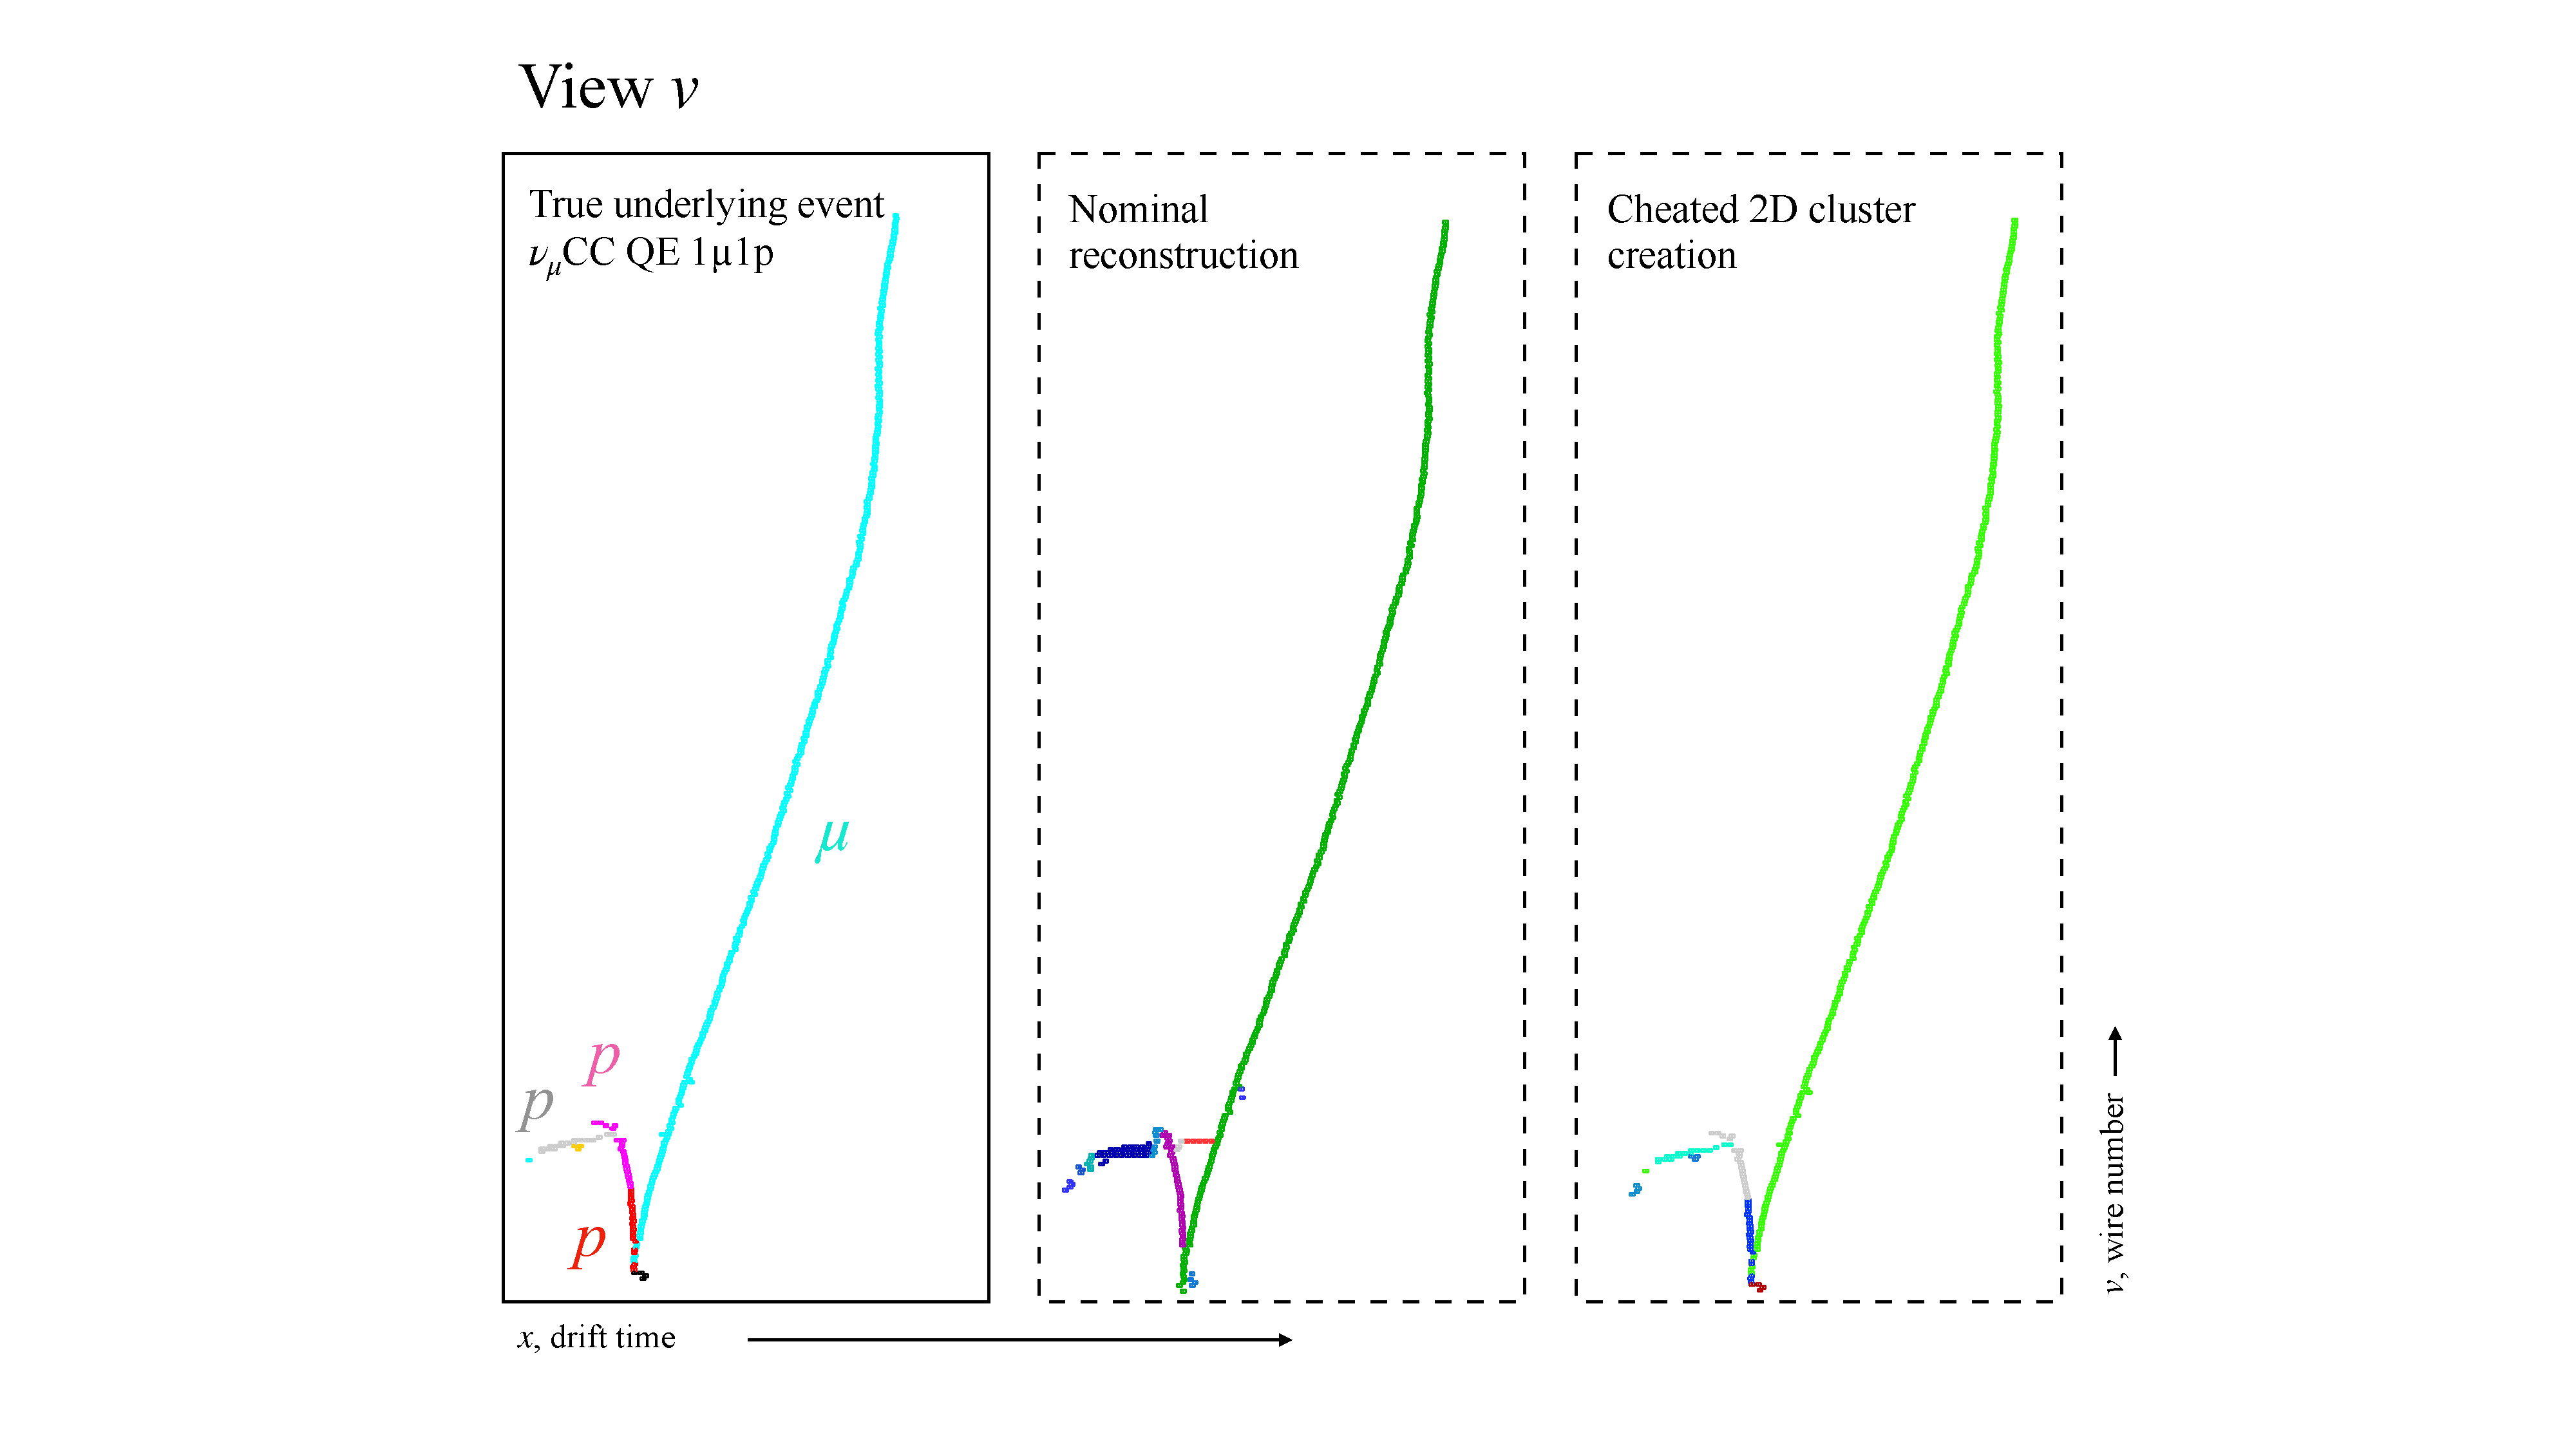
\includegraphics[width=0.85\linewidth, trim={12cm 0 11cm 0}, clip]{pandora/chapter_4/cluster2D.pdf}
    \caption[CheatingClusterCreation versus TrackClusterCreation algorithm]{Illustration of the effect of the CheatingClusterCreation algorithm, with a $1\PGm1\Pp$ event. The reconstruction with the cheated cluster creation (shown in the last panel) is closer to the true underlying event (shown in the first panel). Also, compared to the ``nominal'' reconstruction (shown in the middle panel), the reconstructed interaction appears to have fewer noise hits associated and a more refined set of clusters. }
    \label{fig:CheatingClusterCreation}
\end{figure}

To validate and assess the impact of the CheatingClusterCreation algorithm, we need to define a downstream reconstruction metric. Given that the TrackClusterCreation algorithm objective is to assign the correct hits to the respective track in each plane, two valid metrics are the \emph{hit completeness} and \emph{hit purity} scores. Given the hits on the readout plane, it is possible to define the MC matched hits, as the hits that are associated with the true MCParticle and are also associated by Pandora to the reconstructed so-called PFParticle \begin{equation}
    \mathrm{Matched\ hits} \equiv \mathrm{hits_{MCParticle} \cap hits_{PFParticle}}.
\end{equation} \autoref{fig:hit_pur_eff} illustrates this concept on an event with two particles. The reconstructed PFParticle $j$ has a total of seven hits associated with the Pandora reconstruction, whereas PFParticle $k$ has six; the true MCParticle $j$ has nine hits and $k$ has four. So for Particle $j$ the matched hits are seven, and for particle $k$ the number is four. If we introduce the definition of hit purity and hit completeness as \begin{equation}
    \mathrm{Hit\ purity} \equiv \frac{\mathrm{Matched\ hits}}{\mathrm{hits_{PFParticle}}}, 
\end{equation} and \begin{equation}
    \mathrm{Hit\ completeness} \equiv \frac{\mathrm{Matched\ hits}}{\mathrm{hits_{MCParticle}}}. 
\end{equation} we can say that for the case shown in \autoref{fig:hit_pur_eff} we have a purity of \SI{100}{\percent} and \SI{66.7}{\percent}, and a completeness of \SI{77.8}{\percent} and \SI{100}{\percent}, for the $j$ and $k$ particle, respectively. 

\begin{figure}
    \centering
    % \subfloat[]{
    \begin{tikzpicture}
        \node[] at (0,0) {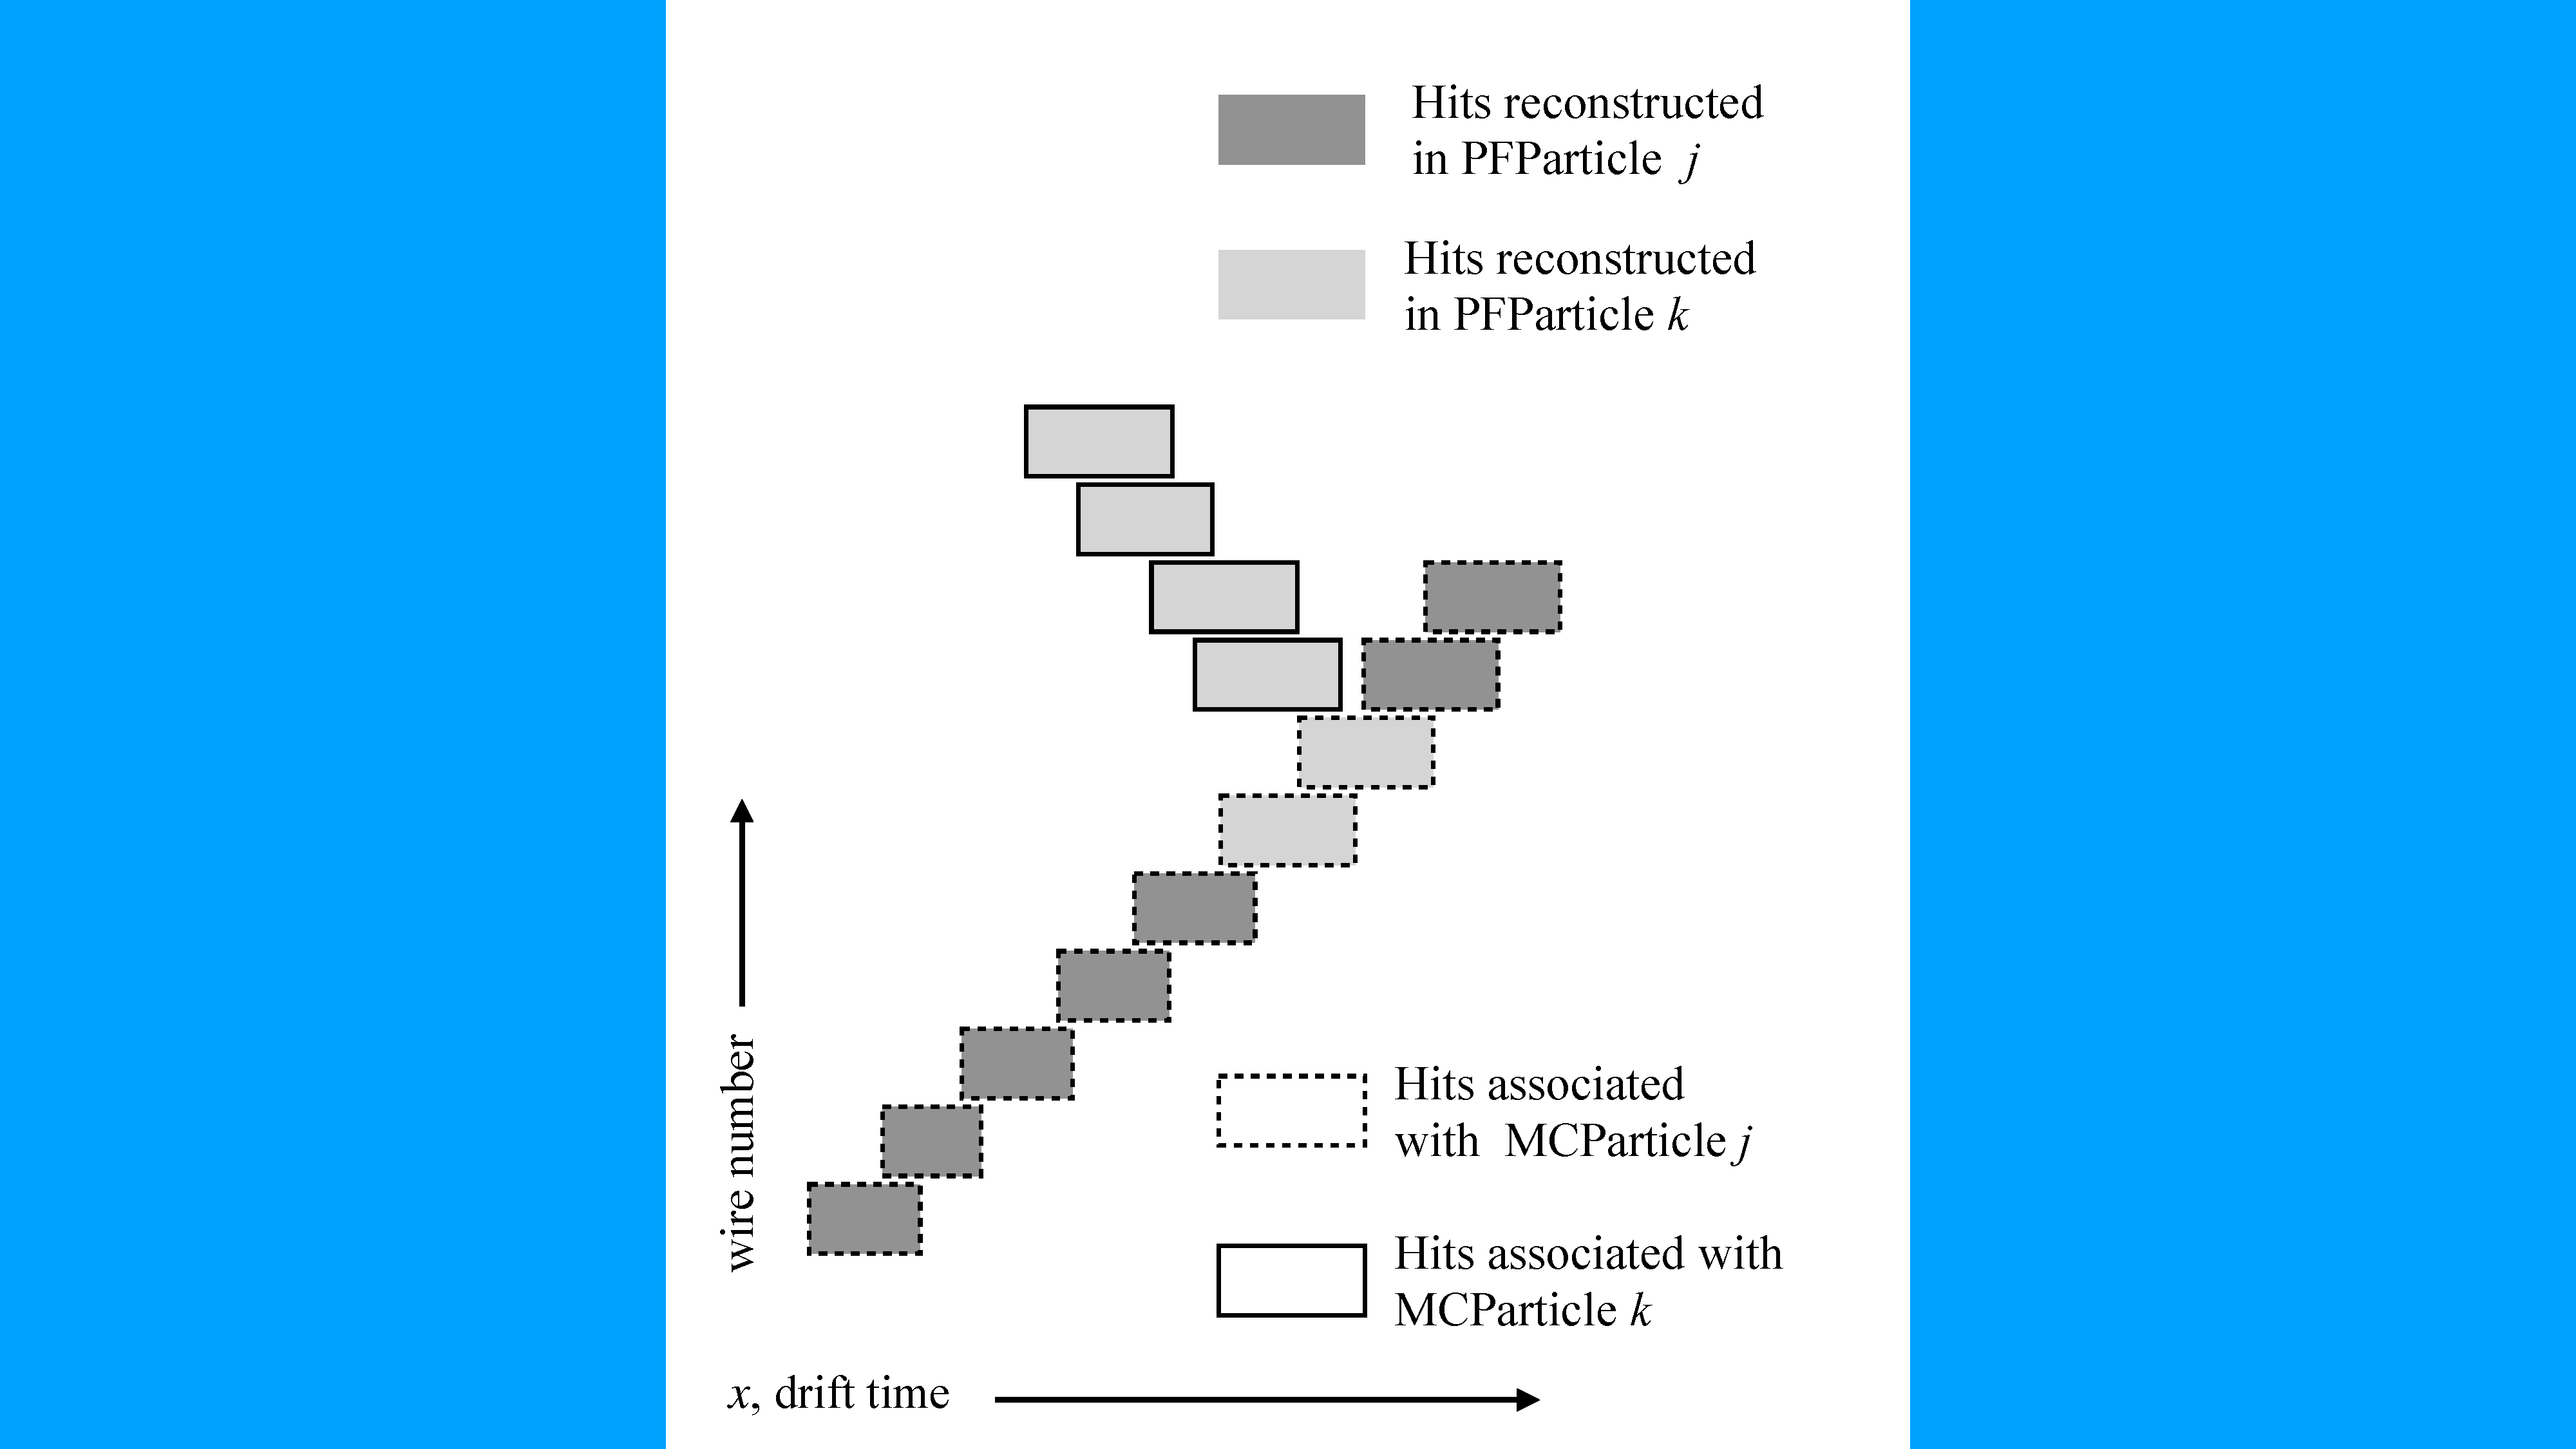
\includegraphics[width=0.5\linewidth, trim={18cm 0 18cm 0}, clip]{pandora/chapter_4/HIT_PUR_EFF.pdf}};
        \node[] at (6, 0) {
        \begin{minipage}[b]{5cm}
            \begin{tabular}{ccc}
                & Particle $j$ & Particle $k$ \\
                $\mathrm{hits_{MCParticle}}$ & 9 & 4 \\
                $\mathrm{hits_{PFParticle}}$ & 7 & 6 \\
                Matched hits & 7 & 4 \\
                Purity & 1 & 0.667 \\
                Completeness & 0.778 & 1
            \end{tabular}
        \end{minipage}
        };
    \end{tikzpicture}
    
    \caption[Definition of hit purity and completeness]{Illustration of the process of hit matching to truth information on an event with two true and two resulting reconstructed particles. More details are provided in the text. }
    \label{fig:hit_pur_eff}
\end{figure}

Given the definitions of hit purity and completeness, we can use them to assess the impact of the CheatingClusterCreation on the event reconstruction. \autoref{fig:hit_purity_completeness_CheatingClusterCreation} illustrates both the hit purity and the hit completeness for a sample of $1\PGm N\Pp$ events selected using the true signal definition \cite{artero_pons_2024_13841852}, for both protons and muons involved in the process. Both hit purity and completeness spectra highlight an improvement in the case of the cheating compared to the nominal 2D clustering algorithm.

\begin{figure}
    \centering
    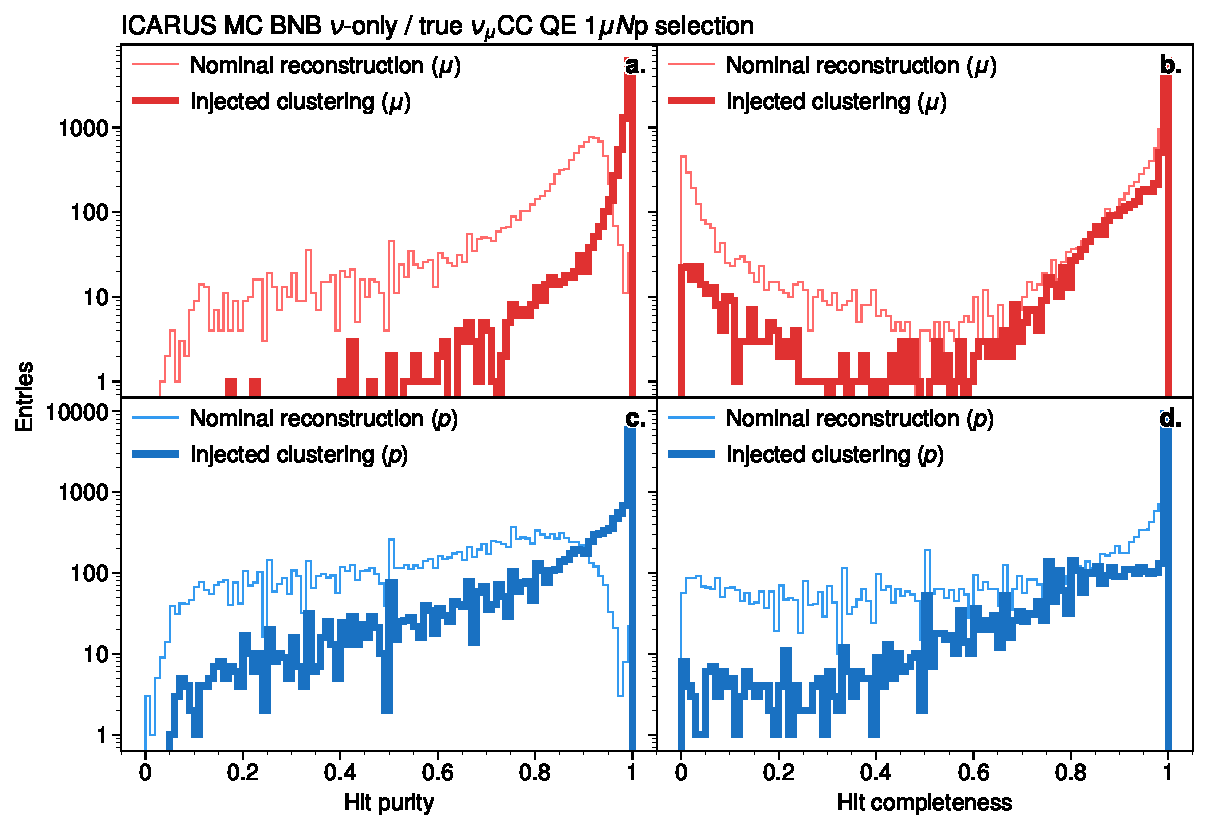
\includegraphics[width=\linewidth]{pandora/chapter_4/toSlide_completeness_purity.pdf}
    \caption[Hit purity and completeness with CheatingClusterCreation algorithm]{Hit purity and hit completeness spectra for the protons (blue) and muon (red) population, for both the cheated cluster reconstruction (thick line) and the nominal reconstruction (thin line).}
    \label{fig:hit_purity_completeness_CheatingClusterCreation}
\end{figure}

However, there is a non-zero fraction of events for which the muon completeness is lower than \num{0.4}. 

Visually scanning these events unveiled that two main issues arise: \begin{enumerate}
    \item Particles have poorly reconstructed hits on some of the wireplanes, making the correct association between views in downstream algorithms tough event if cheating the 2D clustering removes ambiguities at this level;
    \item In some cases, the upstream slice creation fails and splits the muon into two or more slices. The slice that is reconstructed as a $1\PGm N\Pp$ interaction and matches the truly generated one in these cases contains a muon with a smaller than true track length, resulting in a higher hit purity compared to the remaining slices but smaller than one hit completeness.
\end{enumerate} This visual scanning reveals that it is very difficult to decouple the effects of the algorithms upstream in the event reconstruction from the algorithms downstream; since the hit purity and hit completeness metrics are computed downstream of the event reconstruction, these take into account all these effects and are not uniquely affected by the clustering performance. For instance, after the two-dimensional clusters are created, clusters are modified iteratively by the Overshoot- and UndershootTracksTool algorithms that help perform the 3D reconstruction. Similar clustering improvements are performed also before three-dimensional reconstruction is done, once the interaction vertex is created, and after 3D particle creation when the particle refinement tools are run. These downstream operations can cause a cluster to be split into multiple smaller clusters, thus creating multiple reconstructed particles that are matched to the same true particle, thereby undermining the impact of the 2D clustering cheating on the entire event reconstruction. By selecting all the particles that are truth-matched to a muon in the interaction, one recovers the entire muon track. So, it is evident that these events, showing a smaller hit completeness for both protons and muons, are not directly a result of an issue of the CheatingClusterCreation algorithm but more related to issues upstream (i.e., signal processing on the readout planes) or downstream (i.e., 3D reconstruction) of the CheatingClusterCreation algorithms. 
Comparing the hit completeness with the number of reconstructed hits on the collection plane, left and right plots in \autoref{fig:CompletenessVsHits}, it is possible to double-check that low hit completeness values are related to a small number of reconstructed hits. 

\begin{figure}
    \centering
    \subfloat[]{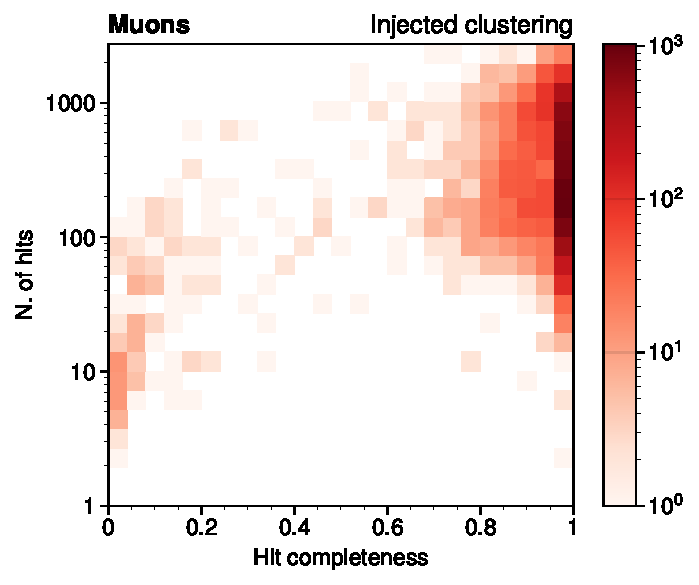
\includegraphics[width=0.5\linewidth]{pandora/chapter_4/muonCompletenessVsHits_cheated2d.pdf}\label{fig:muonCompletenessVsHits_cheated2d}}
    \subfloat[]{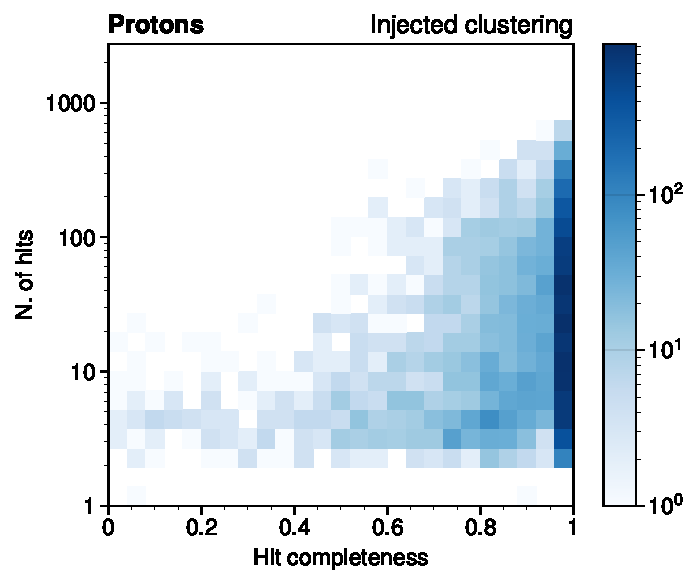
\includegraphics[width=0.5\linewidth]{pandora/chapter_4/protonCompletenessVsHits_cheated2d.pdf}\label{fig:protonCompletenessVsHits_cheated2d}}
    \caption[Hit completeness versus number of hits on collection plane]{Number of hits reconstructed on the collection plane  and associated with a reconstructed particle versus the hit completeness of the same reconstructed particle. The left plot shows the reconstructed particles associated with true muons, whereas the right one shows the same quantities for the protons. Both plots are generated for the case of performing the cheating of the cluster creation. }
    \label{fig:CompletenessVsHits}
\end{figure}

\autoref{fig:lowCompleteness_sliceErr} shows a case in which reconstruction issues are due to failure in the slice creation step/process, resulting in a less than 0.5 hit completeness for the reconstructed muon.

\begin{figure}[!htb]
    \centering
    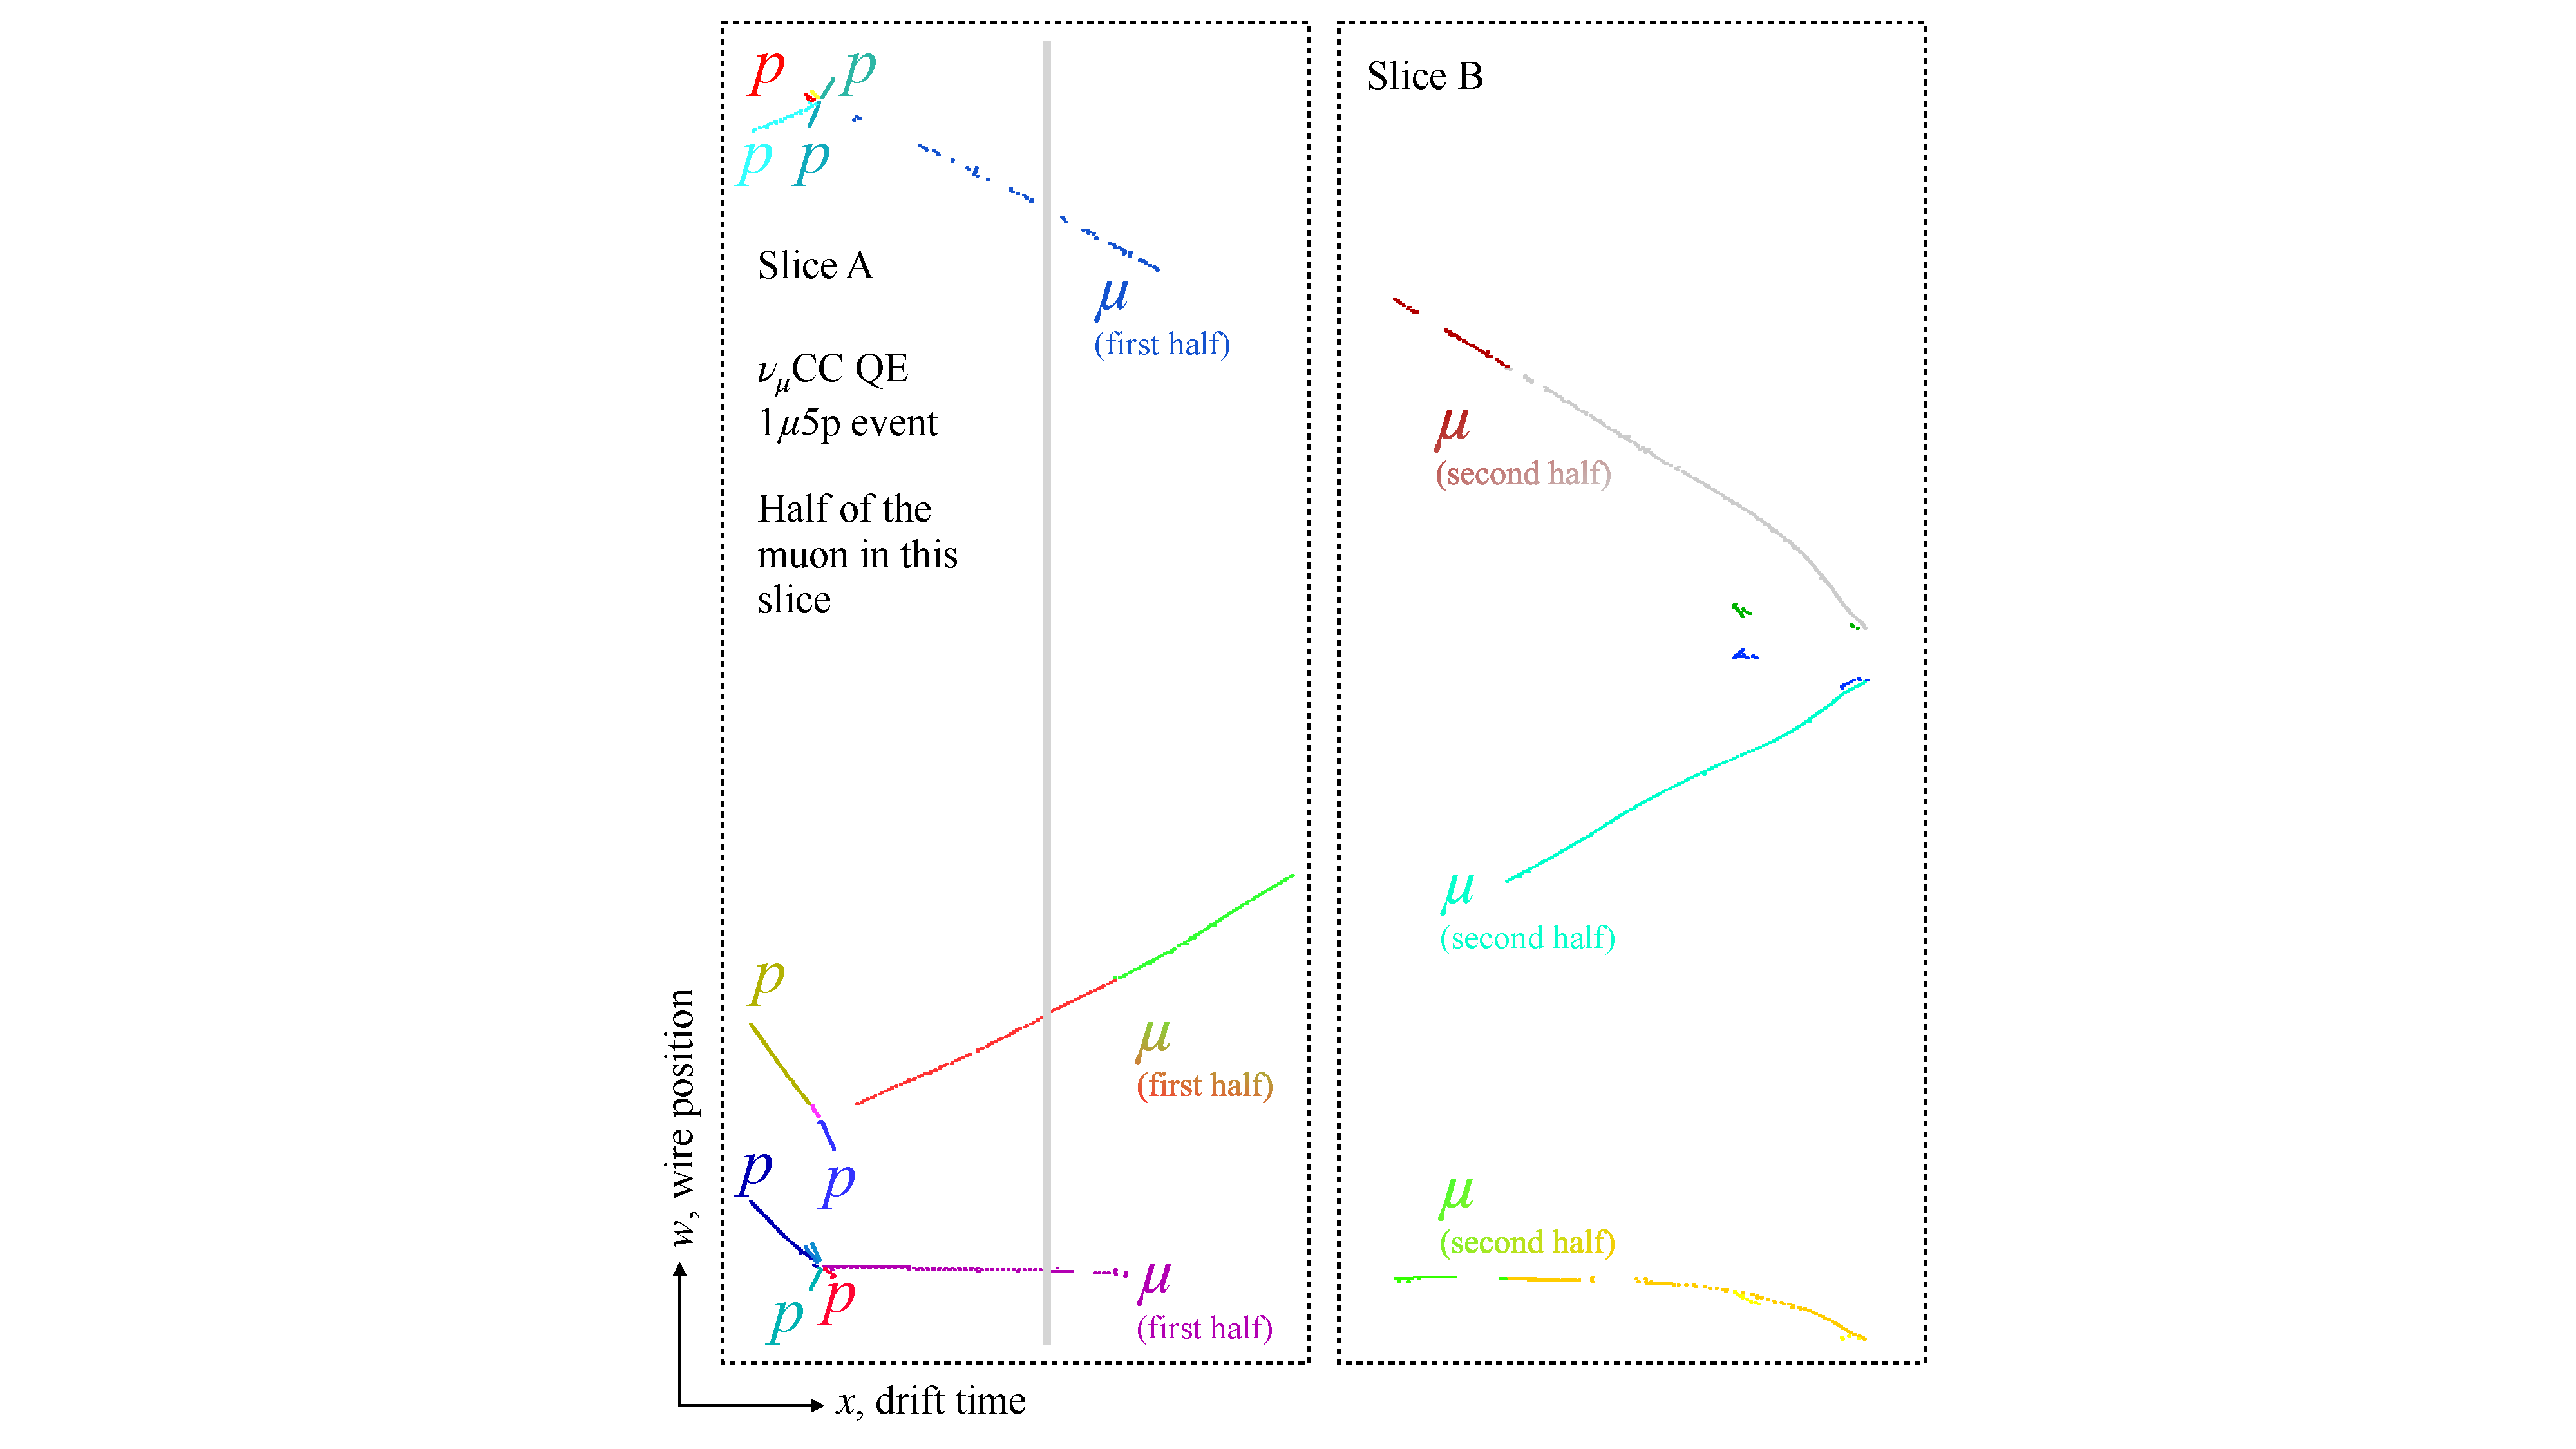
\includegraphics[width=0.75\linewidth, trim={17cm 0 17cm 0}, clip]{pandora/chapter_4/lowCompleteness_sliceErr.pdf}
    \caption{Example of an event for which the reconstructed muon completeness is lower than $0.4$, i.e., $\PGm_\mathrm{completeness} \simeq \num{0.318}$. In this case the lower completeness is due to the true muon particle being split into two slices, of which only one (slice A) is reconstructed as corresponding to a $1\PGm5\Pp$ interaction and thus selected as a signal candidate. }
    \label{fig:lowCompleteness_sliceErr}
\end{figure}

\subsection{Three-dimensional vertex}

Recalling the description of the vertex reconstruction provided in \autoref{sec:TPC_reco_gen}, two algorithms are mostly involved. The first, the CandidateVertexCreation algorithm, performs the creation of two candidate vertices for each 2D cluster created, comparing pairs of clusters from two different readout planes, therefore providing a list of all the ``candidate vertices'' in the interaction. The second, the BdtVertexSelection algorithm, selects from the list of candidate vertices the most probable interaction vertex, using a BDT algorithm and some geometric variables extracted from the clusters and the candidate vertices. 

There are two ways true information can be used to inform the reconstruction of the interaction vertex. 
The most intuitive cheating mode is represented by the replacement of both steps in the vertex identification (candidates creation and final selection) with the assignment of the true 3D position of the interaction vertex from Monte Carlo simulation. This operation is performed by the CheatingVertexCreation algorithm that replaces all the vertex creation and selection algorithms in the XML steering configuration. 

\begin{figure}[!htb]
    \centering
    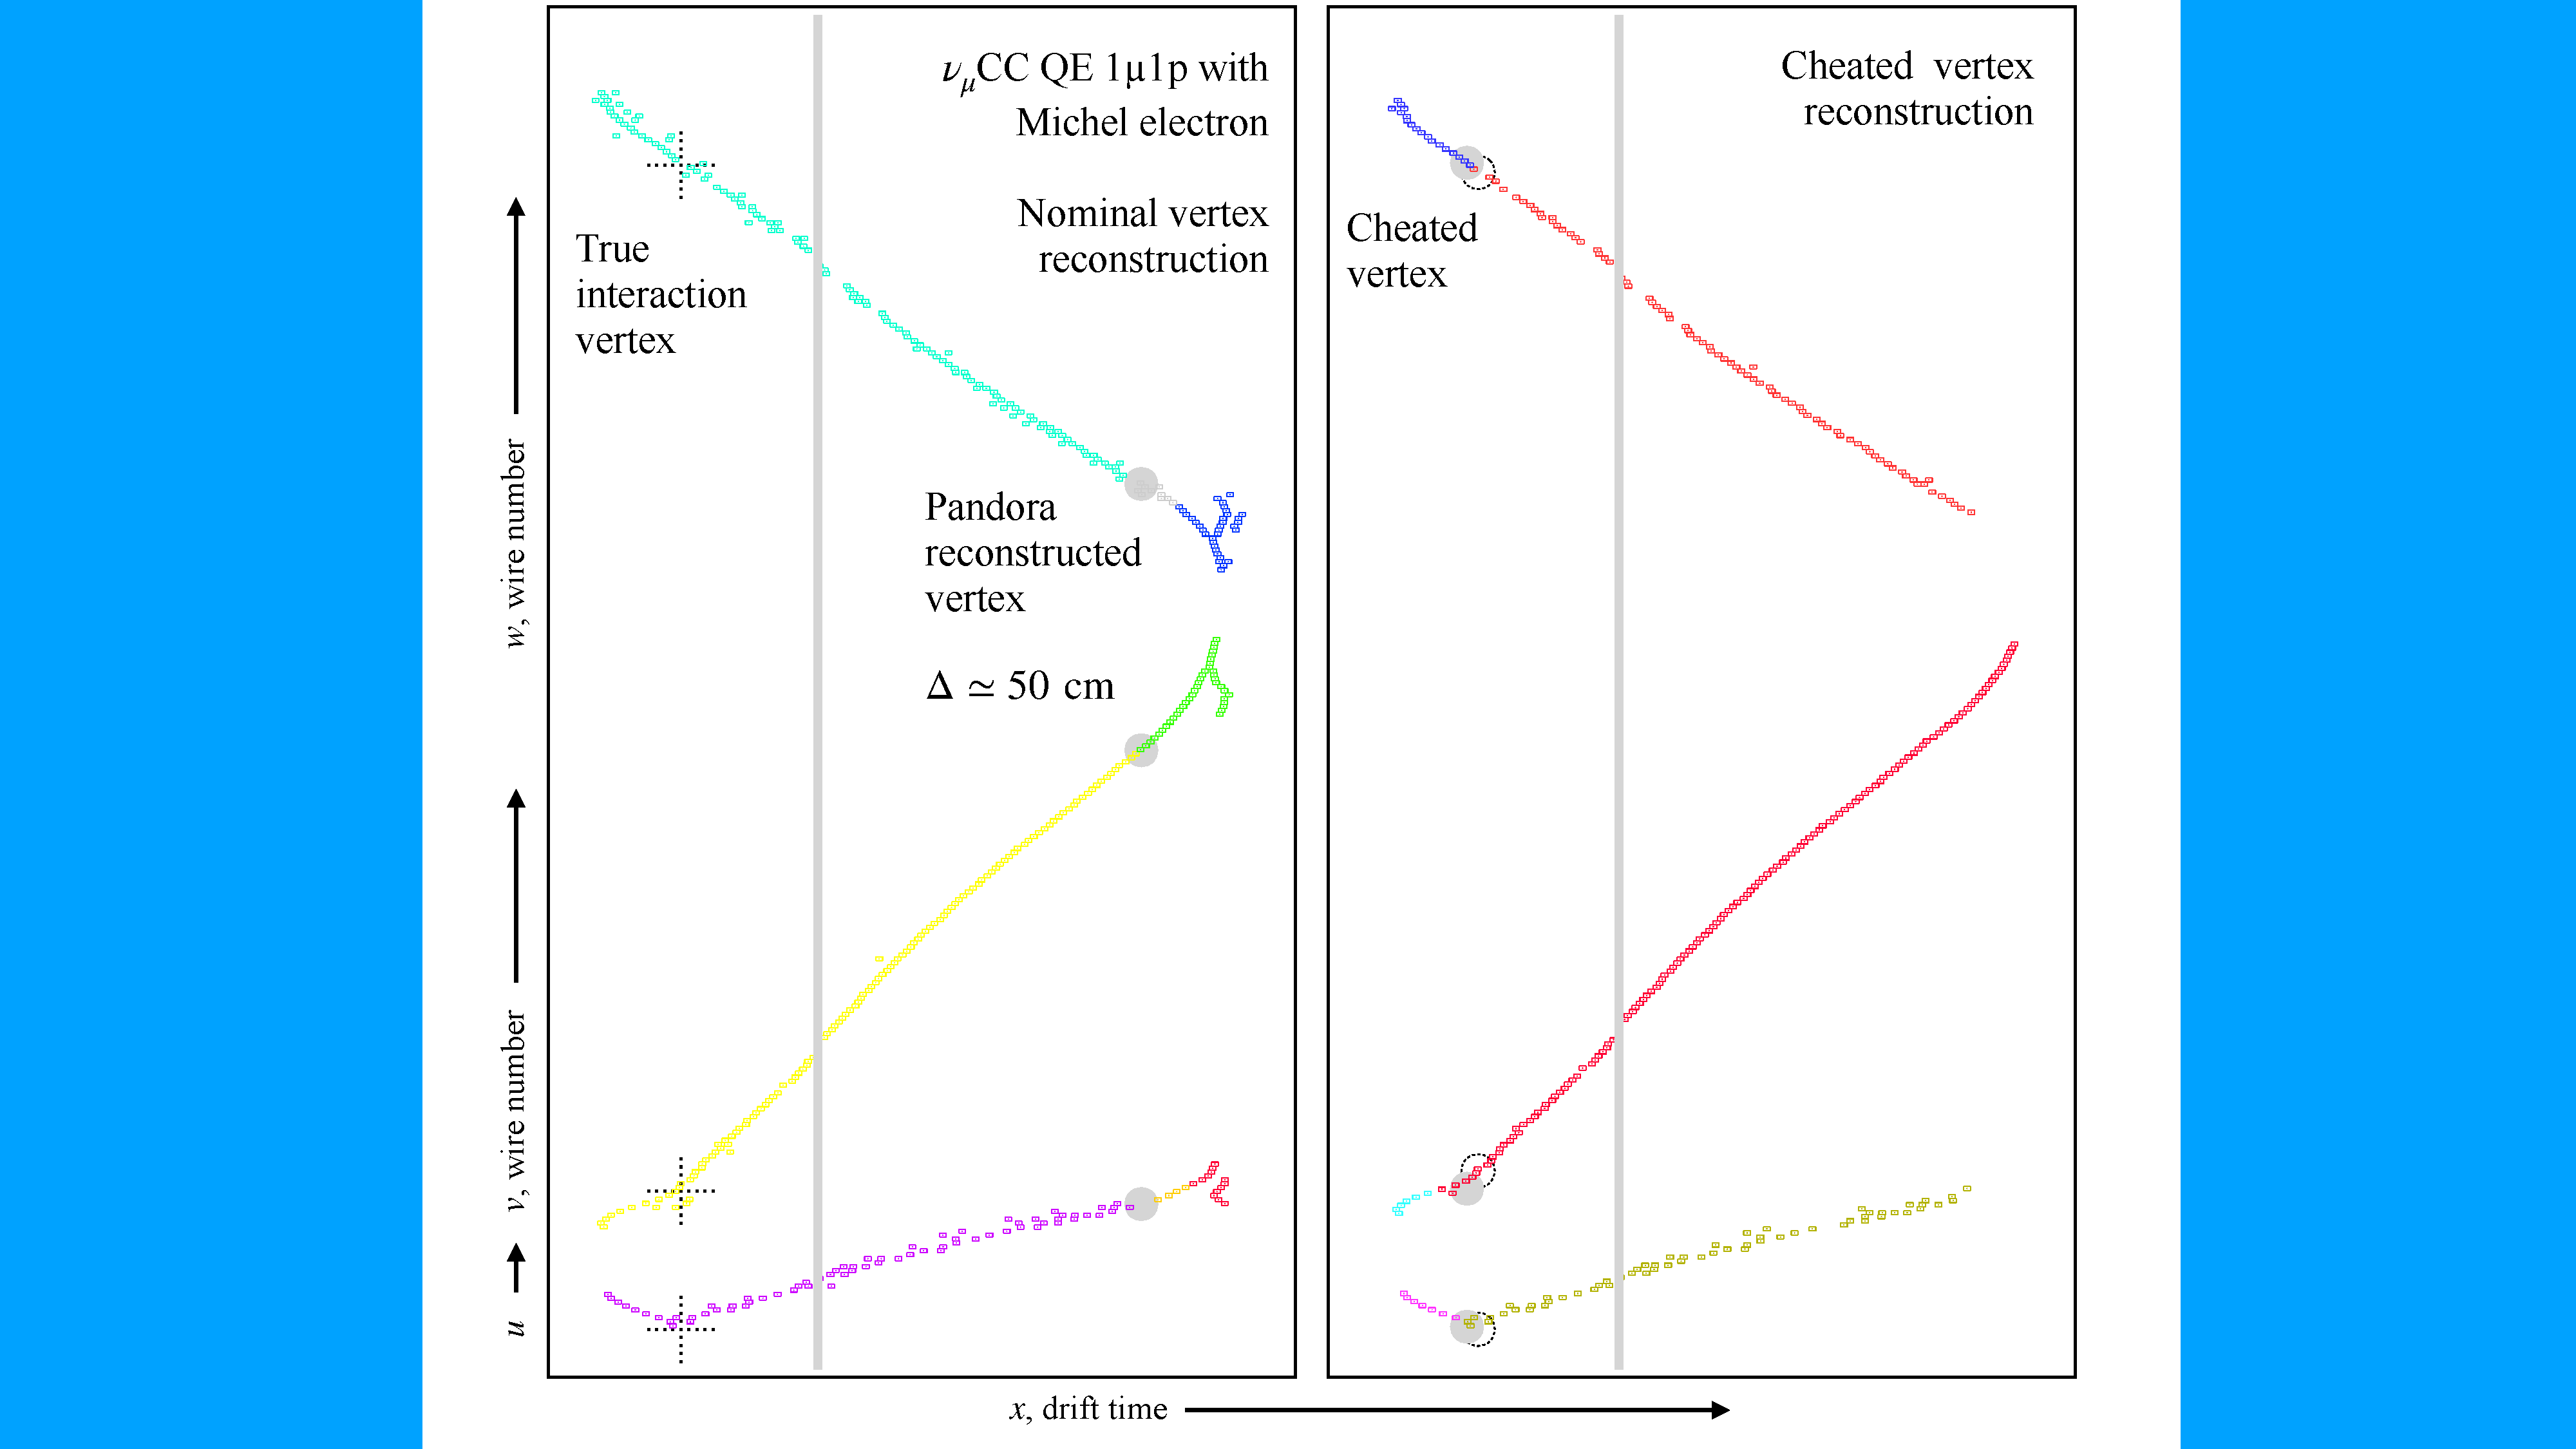
\includegraphics[width=0.95\linewidth, trim={12cm 0 11cm 0}, clip]{pandora/chapter_4/vertex.pdf}
    \caption[CheatingVertexCreation and CheatingVertexSelection algorithms]{Illustration of the impact on Pandora reconstruction of the CheatedVertexCreationAlgorithm. On the left panel, showing the nominal vertex reconstruction, the true neutrino interaction vertex is shown by a dotted cross $+$, whereas the filled circle ($\circ$) indicates the Pandora-reconstructed neutrino interaction vertex. In this case, vertex identification fails, resulting in a (3D) distance between true and reconstructed vertex of half a metre. In the right panel, the outcome of cheating vertex identification is shown, and, as expected, the filled circle matches the true interaction vertex. Additionally, the vertex selected by the CheatingVertexSelection algorithm is shown with a dashed circle. }
    % This is a $1\PGm1\Pp$ event where the primary proton (short track) and the muon (long track) are produced nearly back-to-back. The muon decay producing a Michel electron. 
    \label{fig:CheatingVertexCreation}
\end{figure}

\autoref{fig:CheatingVertexCreation} shows an example of an event where the nominal reconstruction misplaces the interaction vertex. The event is a $1\PGm1\Pp$ event where the primary proton (short track) and the muon (long track) are produced nearly back-to-back. The muon decays in argon, thereby generating a Michel electron. Due to the topological features of the interaction, the vertex in the nominal reconstruction is placed at a distance of ${\sim}\SI{50}{\cm}$ from the true position. Using the CheatedVertexCreation algorithm, the correct interaction vertex is assigned, as shown in the right panel of \autoref{fig:CheatingVertexCreation} where the true and reconstructed vertices coincide.
It is worth noting that the impact of correct vertex reconstruction on the following steps of particle cluster creation is drastic: In the example shown in \autoref{fig:CheatingVertexCreation}, the proton (the particle on the left side of the vertex) is not reconstructed in the nominal case while correctly identified when the vertex reconstruction is cheated.

However, there are some caveats to take into account when evaluating vertex reconstruction performance. Since Pandora operates its algorithms on the reconstructed and filtered hits, it can only add vertices at the endpoint of 2D clusters. However, there are cases where the true interaction vertex position does not correspond to any reconstructed hits. This can happen in these three noteworthy cases: \begin{enumerate}
    \item the interaction vertex lies outside the active volume of the TPC, therefore not producing any signal in the wires in its vicinity;
    \item the conversion gap (i.e., the distance of the first visible hit from the interaction vertex) for the final state particles involved in the interaction is large due to the underlying physics (for example, the production of a $\PGpz$, that is detected through the identification of two $\PGg$ yielding electromagnetic showers in LAr);
    \item the hits near the true interaction vertex are lost in the signal processing stage that takes place before Pandora performs hierarchy reconstruction upon the event. 
\end{enumerate}

\begin{figure}
    \centering
    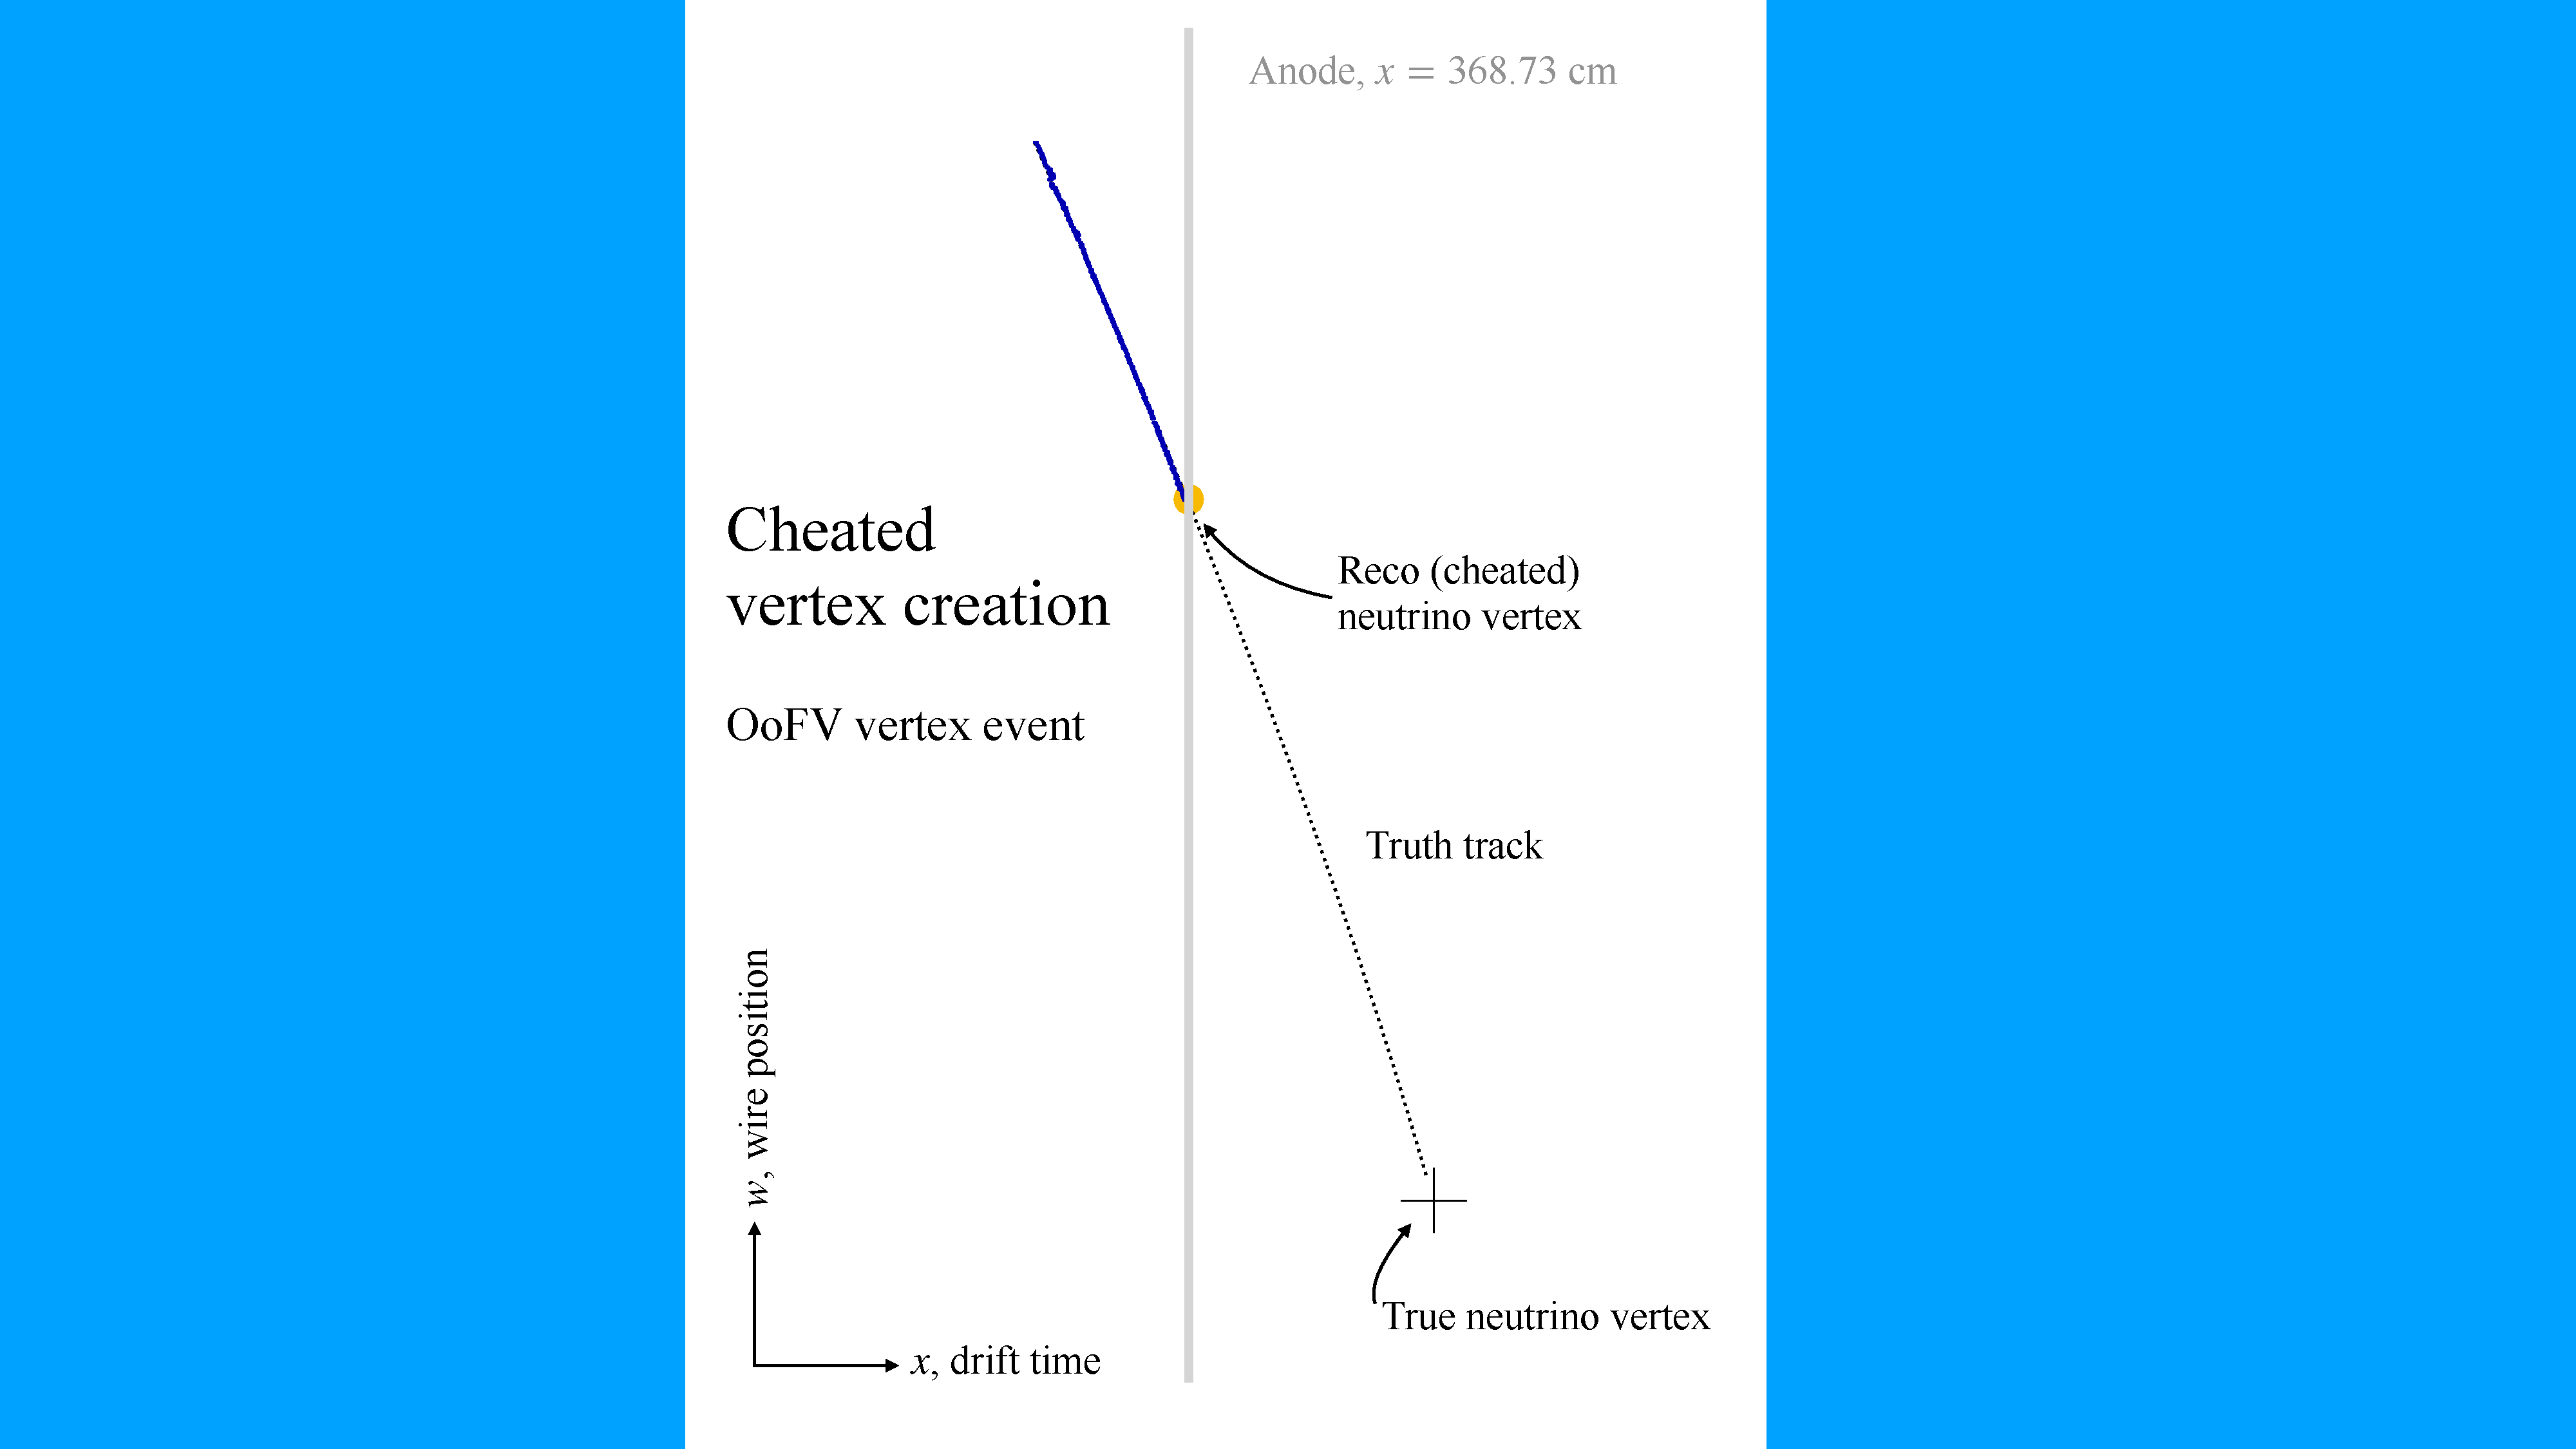
\includegraphics[width=0.55\linewidth, trim={18.5cm 0 22cm 0}, clip]{pandora/chapter_4/vertex_OoFV.pdf}
    \caption[CheatingVertexCreation with an OoFV vertex]{The illustration shows an example of events where the simulated vertex lies and the outcome of cheating vertex reconstruction. As discussed in detail in the text and expected, the position of the reconstructed vertex does not match the true one. }
    \label{fig:CheatingVertexCreation_errors}
\end{figure}

In all these cases, cheating the vertex with the CheatingVertexCreation algorithm results in a vertex placement far from reconstructed hits on the three views. Pandora algorithms downstream of the vertex creation operate on the events and partially solve any ambiguity left by assigning the vertex to the closest hit in 3D space. \autoref{fig:CheatingVertexCreation_errors} shows one of the mentioned cases. In this example, the simulated true vertex is outside the fiducial volume (hence out of the active TPC volume), and the candidate vertex reconstructed and identified by Pandora is highlighted yellow, far from the true position. It is worth remarking that events showing such problems (called \emph{dirt events}) are excluded from the sample of events used in this work, by requiring the vertex to be contained in the fiducial region of the TPC active volume; therefore, such problems do not arise in future results. 

A second point where the true Monte Carlo information can be used to inform the vertex algorithms, and thus a second possible cheating mode of the vertex identification, is the selection of the correct interaction vertex from the list of candidates created by the nominal CandidateVertexCreation algorithm. This operation essentially entails bypassing the BDT performing the choice and selecting, from the list of vertex candidates created as described in \autoref{sec:PandoraNeutrino}, the vertex which lies closest to the true interaction vertex. \autoref{fig:CheatingVertexCreation}, on the right panel, shows the result of cheating the vertex selection (dashed circle). 

Validating the cheating of the vertex reconstruction is straightforward: it is possible to check the distance of the true vertex with respect to the reconstructed vertex of the interaction. \autoref{fig:vertex_cheated_dispacement} shows this for both the cheating of the vertex creation (thick black line) as well as the cheating of the vertex selection (thin black line), comparing the two cases with the distribution of the vertex distance when the nominal reconstruction is performed. 

\begin{figure}
    \centering
    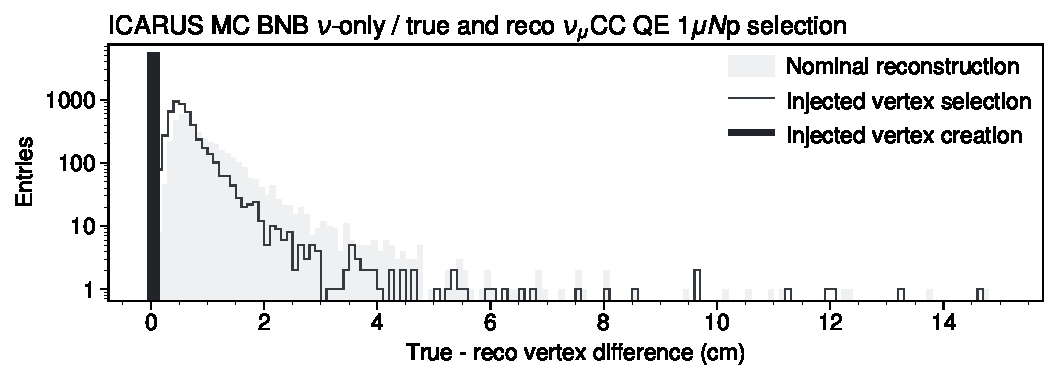
\includegraphics[width=\linewidth]{pandora/chapter_4/toSlide_vertexStudy.pdf}
    \caption[Vertex displacement from truth]{Displacement of the reconstructed vertex from the true vertex, computed when performing the nominal vertex reconstruction (shaded area), cheating the vertex selection (thin black line) and cheating the vertex creation algorithm (thick black line). }
    \label{fig:vertex_cheated_dispacement}
\end{figure}


\subsection{Three-dimensional track and shower reconstruction}

Like the other steps in the reconstruction, cheating the three-dimensional reconstruction steps follows from the nominal version of the algorithm. The idea is that a cheated version of a reconstruction step should replace the nominal version in the chain. This is why the cheating of the three-dimensional reconstruction stage is made of a cheated step, namely the CheatingPfoCreation algorithm, followed by the same ThreeDHitCreation algorithm employed in the nominal version of the reconstruction. In fact, even though the interaction is generated in three-dimensional space, the simulation of the hits is performed only on the 2D readout planes, so there is no possibility to really inject the true $(x,y,z)$ position of each hit, since it is not known. 

The CheatingPfoCreation algorithm goes through all the 2D clusters created by upstream stages of the reconstruction to identify those from each view that share the same true MCParticle. This operation is performed, similarly to the CheatingClusterCreation algorithm, exploiting the MCweight associated with the hits in the cluster. Clusters sharing more than \SI{50}{\percent} of the weighted hits with a given MCParticle are added together. Once they are added together, no further operation is performed other than the geometrical reconstruction, which is performed in the same way it is done for the nominal reconstruction, by creating 3D hits from the sets of 2D clusters. 

It is worth noting that, in order to apply cheating to the 3D matching, the starting point 2D clusters must be as good as they can be. In the nominal reconstruction, the assumption of not fully complete 2D clusters requires the use of the Under-/OverShootTracksTools to remove ambiguous clusters. In the cheated 3D matching, these tools are not run in the standard configuration. In the case of two ambiguous clusters being found on one plane, for example a split cluster, only the cluster with the most shared hits with the true underlying MCParticle will be used, and the remaining cluster is left out of the reconstruction. This is why the cheating of this step of the reconstruction is only performed when the previous steps are also cheated, and not as an individual module. 

\begin{figure}
    \centering
    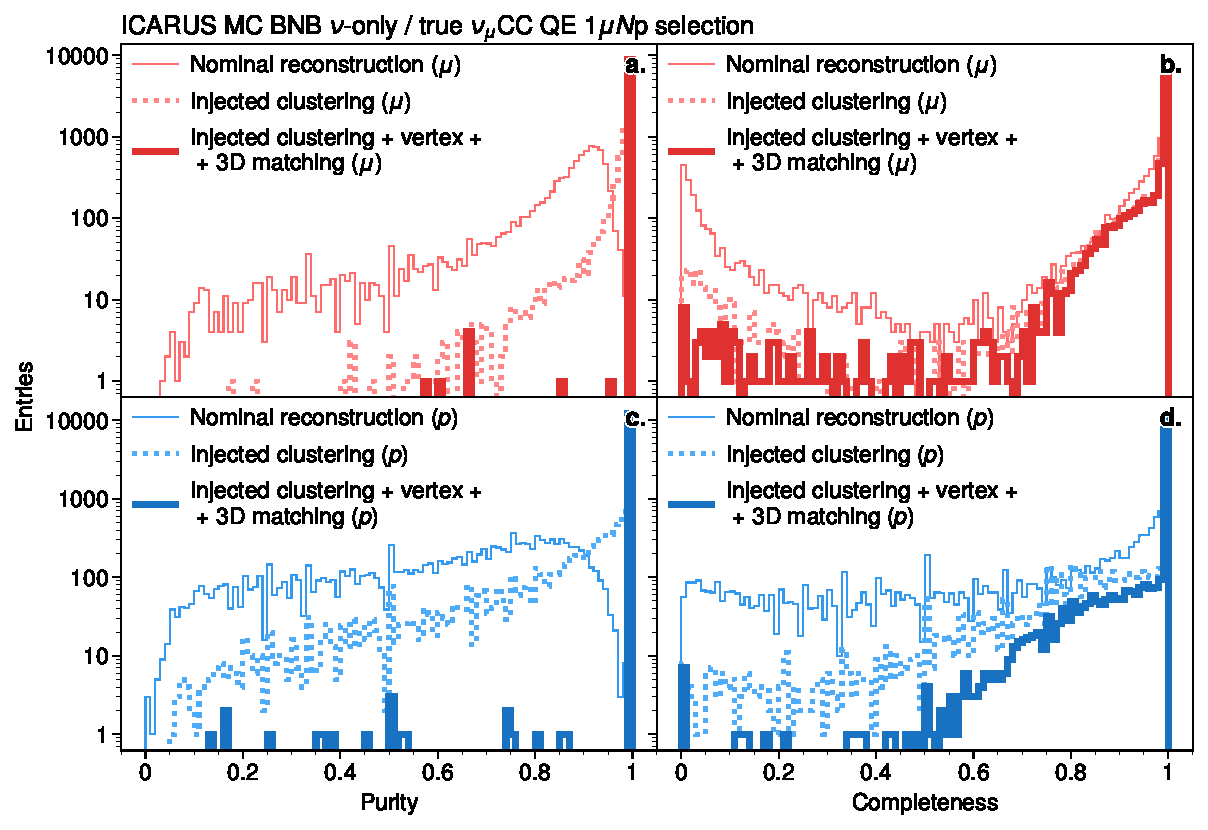
\includegraphics[width=\linewidth]{pandora/chapter_4/toSlide_completeness_purity_3d.pdf}
    \caption[Hit purity and completeness with CheatingPfoCreation algorithm]{Hit purity and hit completeness spectra for the proton (blue) and muon (red) population when the nominal reconstruction is applied (thin line), when the 2D clusters are cheated (dashed line) and when all the steps up to the 3D cluster matching are cheated (thick line).}
    \label{fig:hit_purity_completeness_CheatingPfoCreation}
\end{figure}

To validate the effectiveness of cheating the three-dimensional cluster matching, the same metric as the two-dimensional cluster creation is used. This makes the metric not ubiquitous for either algorithm. However, a smaller, yet not zero, improvement would indicate that the algorithm is performing as expected. This is illustrated in \autoref{fig:hit_purity_completeness_CheatingPfoCreation}, where an improvement with respect to the cheating step of the 2D cluster creation (shown in the dashed line) is visible. 

Similarly to the cheated 2D cluster creation case, a lower hit completeness for both muons and protons is correlated with a lower number of hits in the collection plane, suggesting that either there are more than one reconstructed particles associated with the true underlying MCParticle or that the particle is split into two slices. This is shown in \autoref{fig:CompletenessVsHits_cheated2dVtx3d}, closely matching the same trend that was highlighted for muons and protons when performing the cheating of the two-dimensional cluster creation. 

\begin{figure}
    \centering
    \subfloat[]{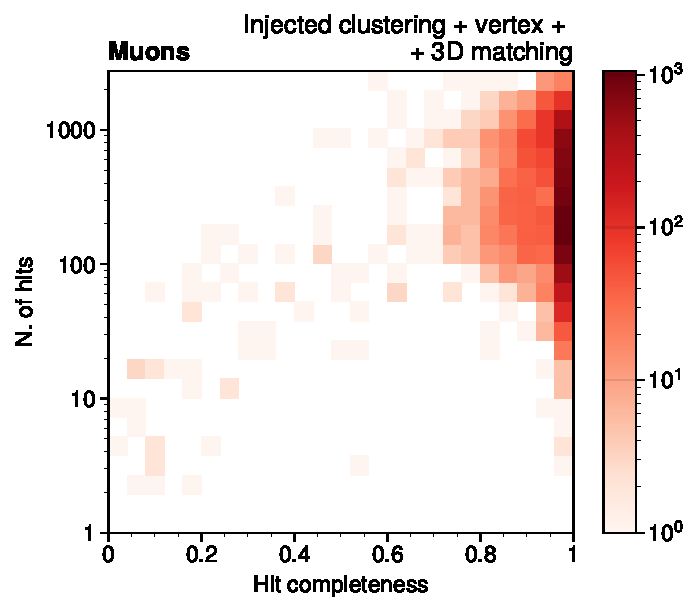
\includegraphics[width=0.5\linewidth]{pandora/chapter_4/muonCompletenessVsHits_cheated2dVtx3d.pdf}\label{fig:muonCompletenessVsHits_cheated2dVtx3d}}
    \subfloat[]{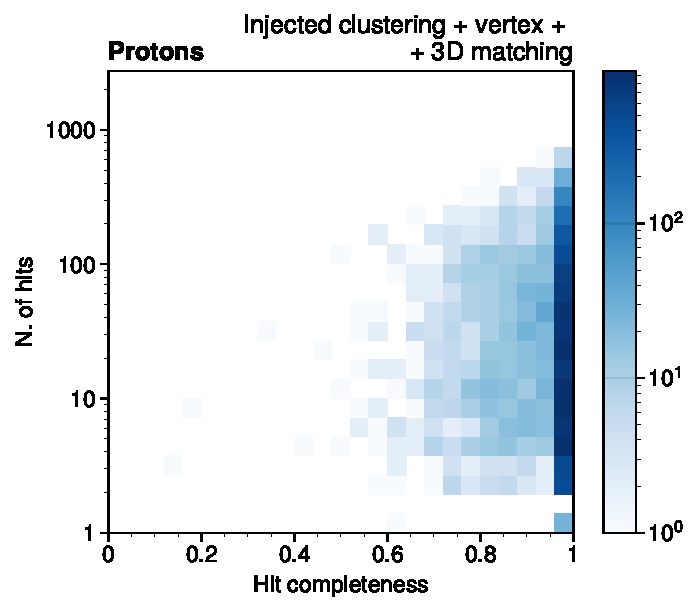
\includegraphics[width=0.5\linewidth]{pandora/chapter_4/protonCompletenessVsHits_cheated2dVtx3d.pdf}\label{fig:protonCompletenessVsHits_cheated2dVtx3d}}
    \caption[Hit completeness versus number of hits on collection plane]{Number of hits reconstructed on the collection plane associated with a reconstructed particle versus the hit completeness of the same reconstructed particle. On the left there are reconstructed particles associated with true muons, whereas on the right there are true protons. Both plots are produced when performing the cheating of the three-dimensional cluster matching and creation. }
    \label{fig:CompletenessVsHits_cheated2dVtx3d}
\end{figure}

\subsection{Particle hierarchy reconstruction} 

The cheating of the particle hierarchy reconstruction, implemented by the CheatingNeutrinoCreation and CheatingNeutrinoDaughterVertices algorithms, aims at assigning the correct parent-daughter relationship to all reconstructed particles in the interaction. Using MCWeights associates a reconstructed particle with the underlying MCParticle that is most compatible. Using this association then assigns the reconstructed neutrino interaction vertex to the reconstructed particles identified as primary from the underlying MCParticle. The same is then performed for secondary particles in the interaction, also assigning the daughter vertices to the daughter particles. 

It is not immediate, given that this step is very downstream of the reconstruction chain, to validate that cheating the particle hierarchy creation is working as planned. As for previous algorithms, it is required that the upstream reconstruction be as perfect as it can be, since the MCParticle-reconstructed particle association is performed using the MCWeights: if an MCParticle gets split into two or more reconstructed particles, only the particle sharing the most weighted hits will be assigned the correct parent-daughter hierarchy.

Ideally, assigning the correct parent-daughter relations would result in more primary particles getting assigned as primary particles. Also, a greater purity of the events selected should be observed: no contamination from reinteracting particles that are not individually reconstructed should be present. Thus, for the $\PGnGm$CC QE Np analysis, cheating the particle hierarchy should result in the proton multiplicity being assigned correctly. \autoref{fig:Np} shows the comparison of reconstructed and true proton multiplicity, highlighting that if the reconstruction is cheated all the way up to the particle hierarchy creation, as shown in \autoref{fig:Np}\ref{sub@fig:Np_cheated_2d_vtx_3d_nu}, the diagonal is more prominent with respect to the nominal reconstruction, shown in \autoref{fig:Np}\ref{sub@fig:Np_nominal}. 

\begin{figure}[!htb]
    \centering
    \subfloat[]{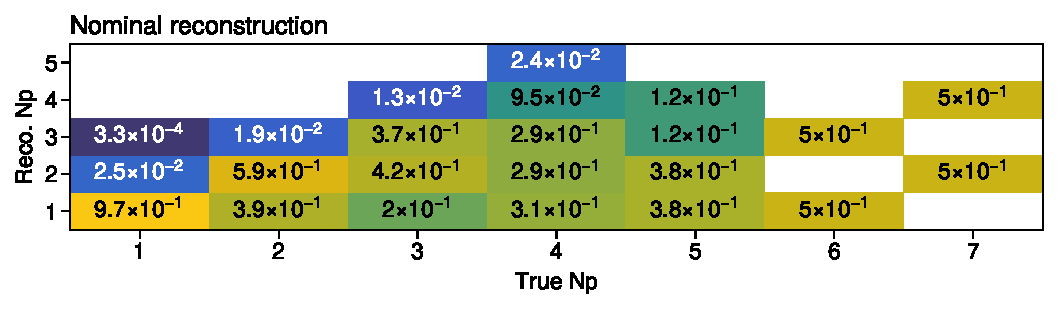
\includegraphics[width=\linewidth]{pandora/chapter_4/Np_comparison_nominal.pdf}\label{fig:Np_nominal}}
    
    \subfloat[]{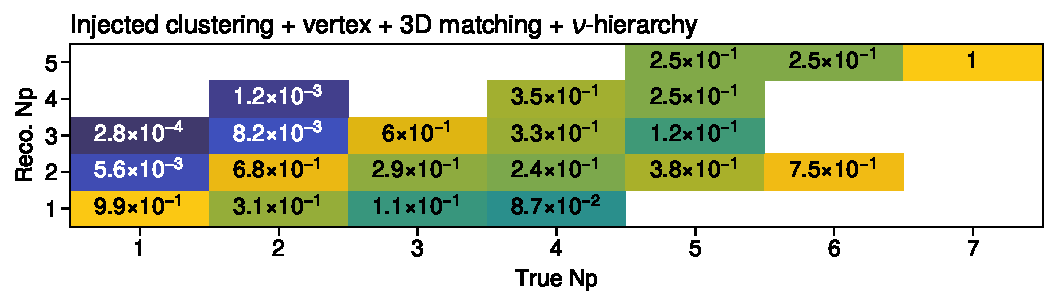
\includegraphics[width=\linewidth]{pandora/chapter_4/Np_comparison_cheated_2d_vtx_3d_nu.pdf}\label{fig:Np_cheated_2d_vtx_3d_nu}}
    \caption[True versus reconstructed primary proton multiplicity]{True versus reconstructed proton multiplicity distribution. The numbers are normalised with respect to the true multiplicity. These plots show that when all the steps of the reconstruction up to the particle hierarchy creation are cheated, more events are assigned the correct number of primary protons. The numbers on the plots are the entries normalised on a column base, i.e, on the true number of protons in the interaction. }
    \label{fig:Np}
\end{figure}

This step is, however, delicate; hence, some remarks are mandatory to better understand the plots. Firstly, although correctly assigning the particle hierarchy is crucial for the downstream event selection, it is not the only piece of the puzzle, as the multiplicity of the reconstructed protons highly depends on the efficiency of the particle identification. Furthermore, in \autoref{fig:Np}\ref{sub@fig:Np_cheated_2d_vtx_3d_nu} there are some cases, especially when the proton multiplicity is higher, where the reconstruction fails to reconstruct the associated hits. This is due to the fact that, if the interaction energy is fixed to that of the incoming neutrino (peaked at \SI{800}{\mega\electronvolt}), more protons in the final state will each have allocated less energy, therefore making the hit reconstruction on the wireplanes more difficult. Finally, given the event selection cuts presented in \autoref{sec:dataSample_and_selection}, two things have to be highlighted: \begin{enumerate}
    \item The present selection relies strongly on this step, since it requires both the muon and the protons identified within the interaction to be primary particles, as well as ensuring that any other particle identified not as a proton or a muon is not primary in the interaction. 
    \item Given that Pandora fails most of the time to identify daughter particles, collapsing them onto the primaries, the event selection was tuned accordingly. This is why in the event selection the requirement for the primary protons to have at least \SI{50}{\mega\electronvolt} of deposited energy was extended, at the truth level, to the proton itself and all its daughter particles, to correctly match the fact that in the signal selection for reconstructed particles those daughter particles were collapsed to the primary. 
\end{enumerate} 

These conditions imply that the event selection does not fully exploit the correct creation of the particle hierarchy. Therefore, altering this step by injecting the true MC information to improve its performances,  does not necessarily have a proportional impact on the reconstruction and selection efficiency. In reality, the situation is diametrically opposed to this: when the true particle hierarchy is injected into the reconstructed particles, there are multiple events that get lost solely due to event selection inefficiencies. 


The issues preventing the correct reconstruction of the particle hierarchy and the correct identification of the interaction are multiple. Here are highlighted two of the most common cases: \begin{itemize}
    \item There are cases where all the particles in the final state are reconstructed. Thus it should be expected the correct particle hierarchy to improve the selection efficiency. However, in such events, the prompt proton, fully reconstructed with high hit completeness and purity, can be shorter than the \SI{2.3}{\cm} lower threshold (equivalent to the $\SI{50}{\MeV}$ threshold) required, even if in the true selection the $E_\mathrm{dep}>\SI{50}{\MeV}$ requisite is fulfilled, since its daughter particles are added into the total computation. An example of this case is found in \autoref{fig:particleHierarchy}\ref{sub@fig:particleHierarchy_lowEProton}. Such events get otherwise selected when performing the cheating up to the stage that performs the three-dimensional reconstruction, since Pandora (mis-)identify the daughter proton of the prompt proton reinteraction as a primary particle. In such cases, the energy difference due to the missing prompt proton is small; hence, the event selection does not reject the event. 
    
    \item Another possibility is having the prompt proton produce visible hits only on one readout plane. This also happens for very short prompt protons that reinteract in LAr, producing a daughter proton. \autoref{fig:particleHierarchy}\ref{sub@fig:particleHierarchy_missingHits} illustrates this failure mode with an example. In this case, the prompt proton is not reconstructed (Pandora requires at least two planes to perform a three-dimensional reconstruction). If the particle hierarchy creation is left nominal, its daughter particle gets assigned as a primary particle of the interaction vertex. When the particle hierarchy is, however, cheated, the correct hierarchy is assigned, therefore resulting in an event with no primary proton $1\PGm0\Pp$: such an event gets rejected by the event selection.
\end{itemize}

\begin{sidewaysfigure}
    \centering
    \subfloat[]{\includegraphics[height=8cm, trim={10cm 0 22cm 0}, page=2]{pandora/chapter_4/particle_hierarchy_error.pdf}\label{fig:particleHierarchy_lowEProton}}
    \subfloat[]{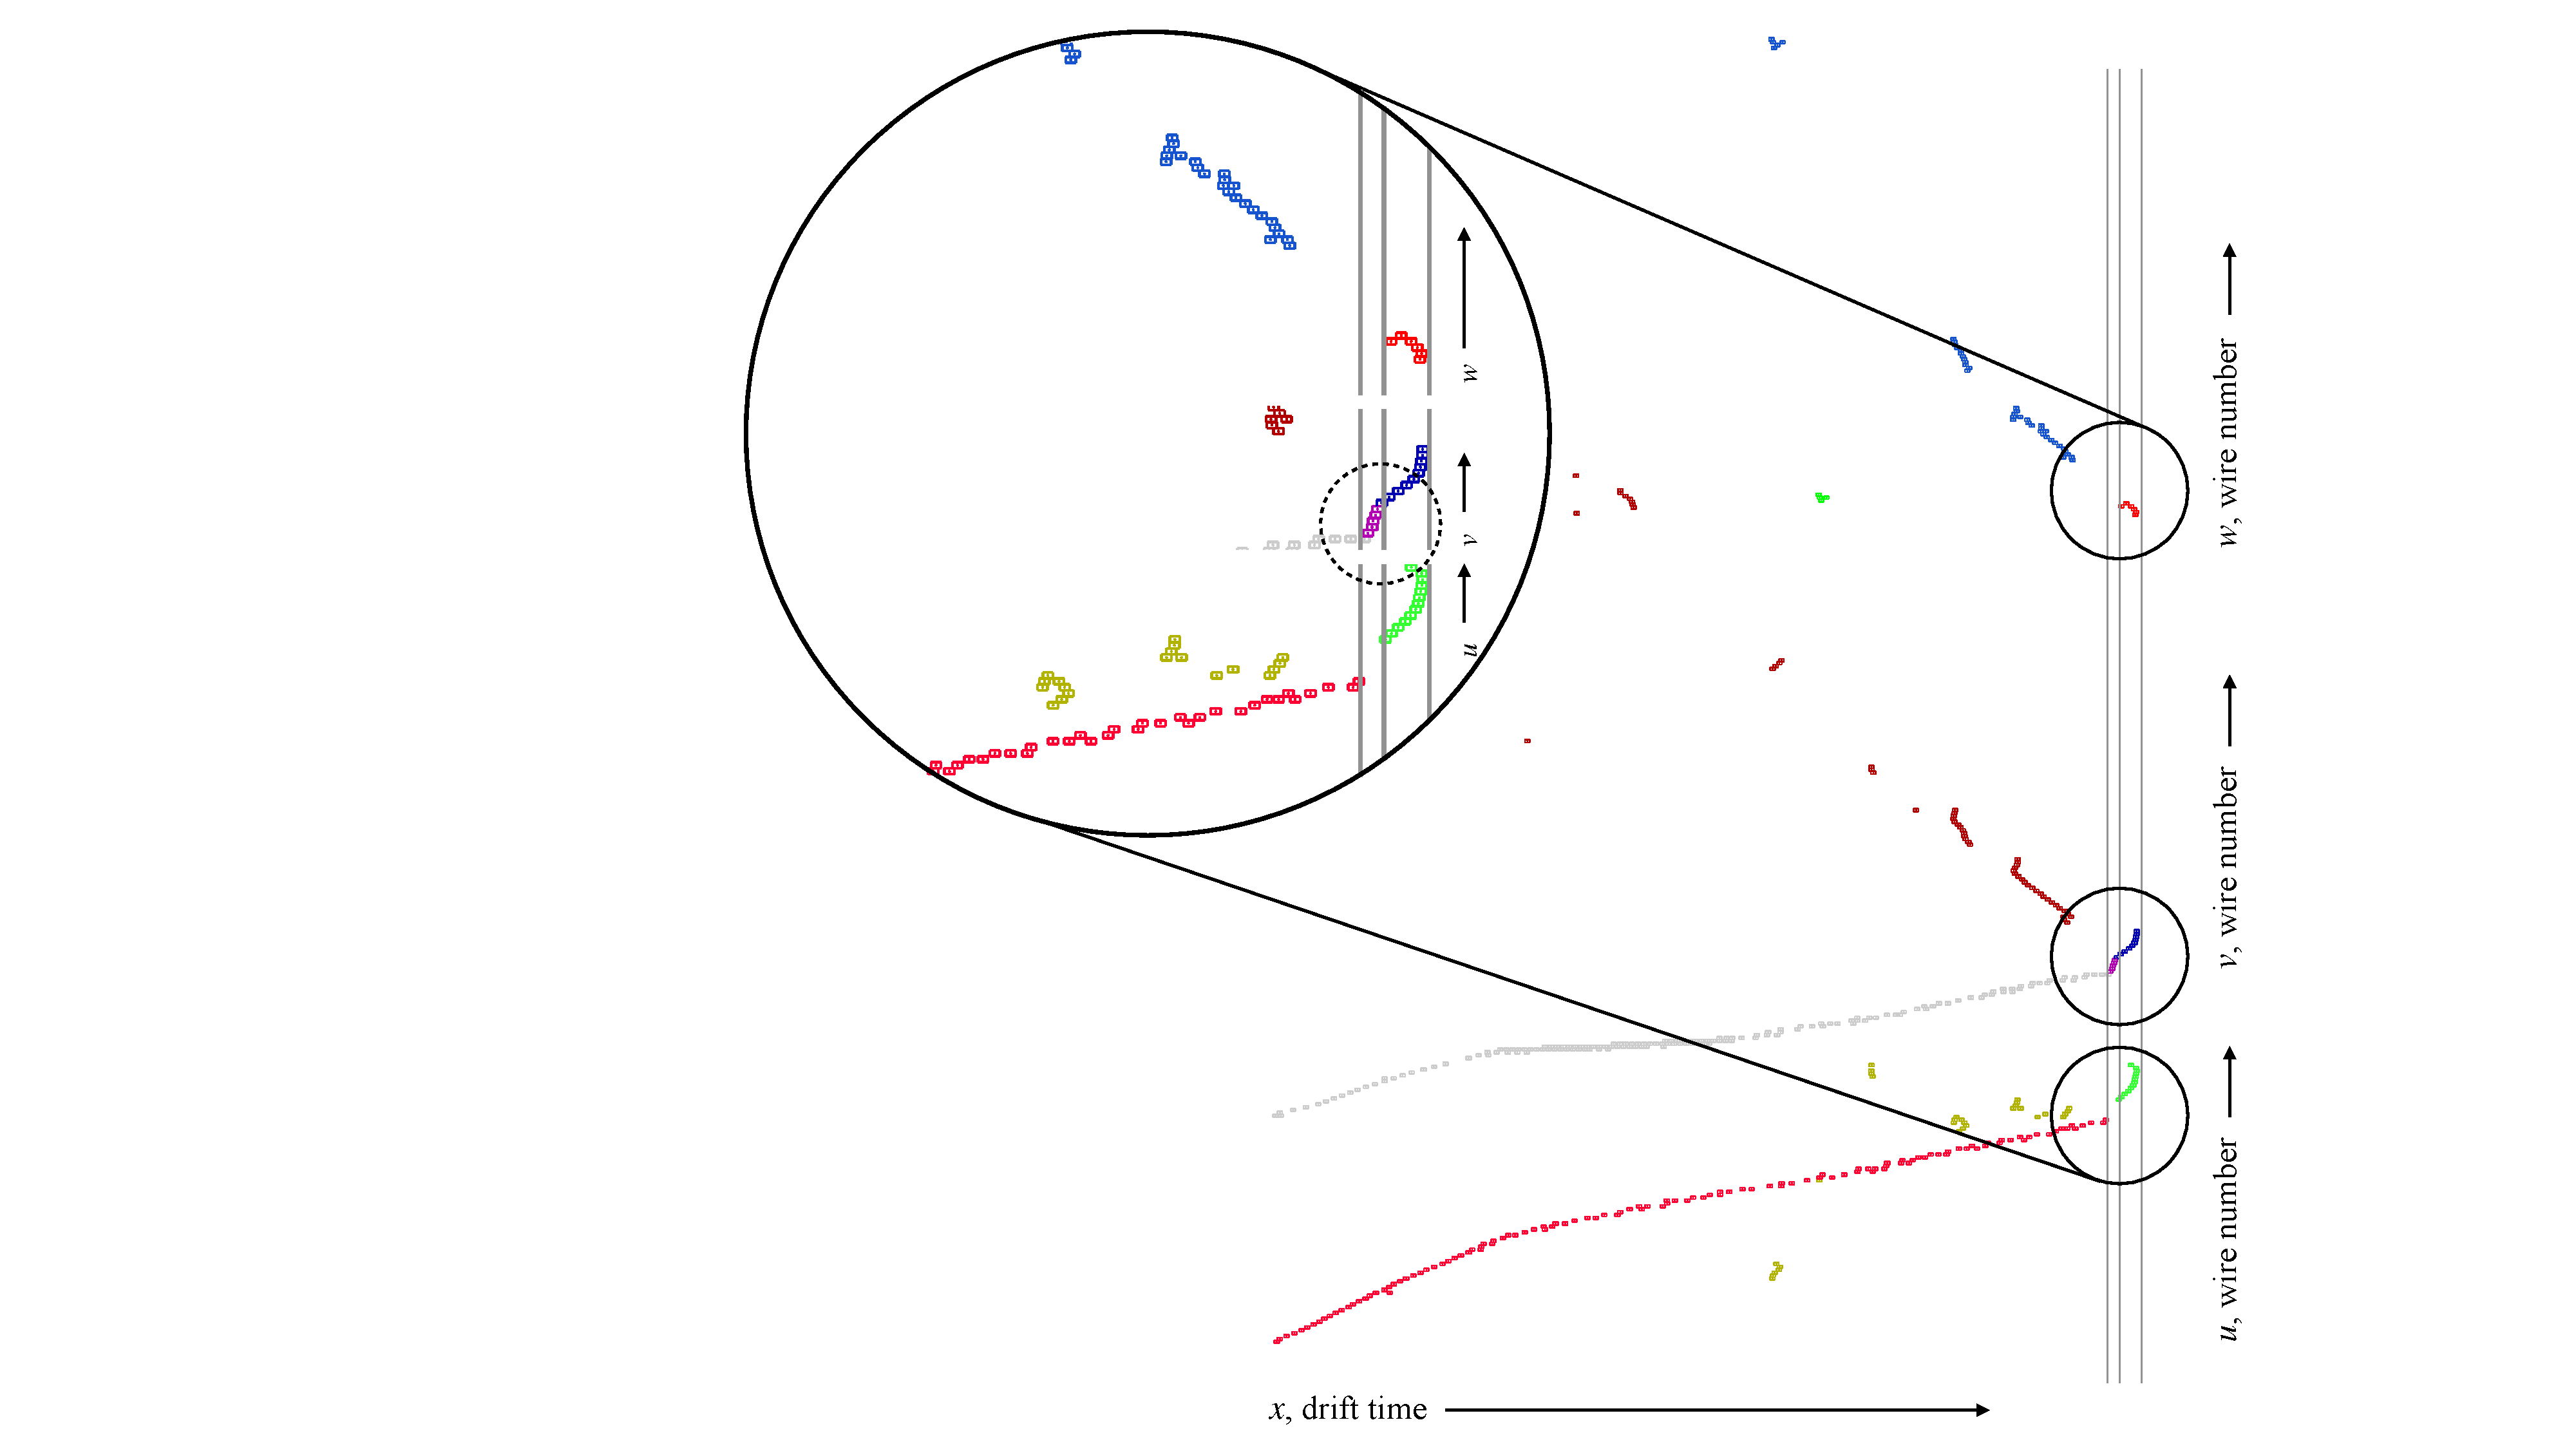
\includegraphics[height=8cm, trim={22cm 0 8cm 0}, page=1]{pandora/chapter_4/particle_hierarchy_error.pdf}\label{fig:particleHierarchy_missingHits}}
    \caption[Particle hierarchy cheating failure modes]{\ref{sub@fig:particleHierarchy_lowEProton} illustrates one event where the primary (prompt) proton is shorter than the lower threshold of \SI{2.3}{\cm} or equivalently \SI{50}{\MeV} of deposited energy. This event is therefore not selected if the daughter proton of the prompt proton is assigned the correct parent-daughter hierarchy, like when performing the cheating of the particle hierarchy. \ref{sub@fig:particleHierarchy_missingHits} illustrates the case where the prompt proton is not reconstructed due to missing information on some of the readout planes. This event is not selected since the secondary proton, daughter to the prompt proton, is not identified as primary when the particle hierarchy is cheated. }
    \label{fig:particleHierarchy}
\end{sidewaysfigure}



Having deeply studied the effect of cheating the particle hierarchy creation algorithm, it was then chosen, for the purpose of this thesis, to leave this step of the reconstruction nominal, therefore not implementing it in any further studies. 

\subsection{Particle classification}

The last step of the PandoraNeutrino reconstruction path, aimed at classifying particles, based solely on topological features, into tracks or electromagnetic showers, can be cheated in two different ways. 

The easiest way is to just take the Particle Data Group (PDG) code, uniquely identifying each MC particle with a label and assigning it correctly to the reconstructed particle. This is the way that it was originally implemented in the Pandora chain but proved not very useful to the tests performed in this work, since the event selection for the $\PGnGm$CC QE Np analysis, used downstream of the event reconstruction, does not rely on this information but instead makes use of the track/shower classification BDT score that is produced by the nominal reconstruction algorithm. So another way of cheating this stage of the reconstruction was implemented as part of this work. This implementation uses the true PDG label associated with MCParticles to cheat the value of the BDT track score, effectively making the track-shower separation perfect. 

\begin{figure}[!htb]
    \centering
    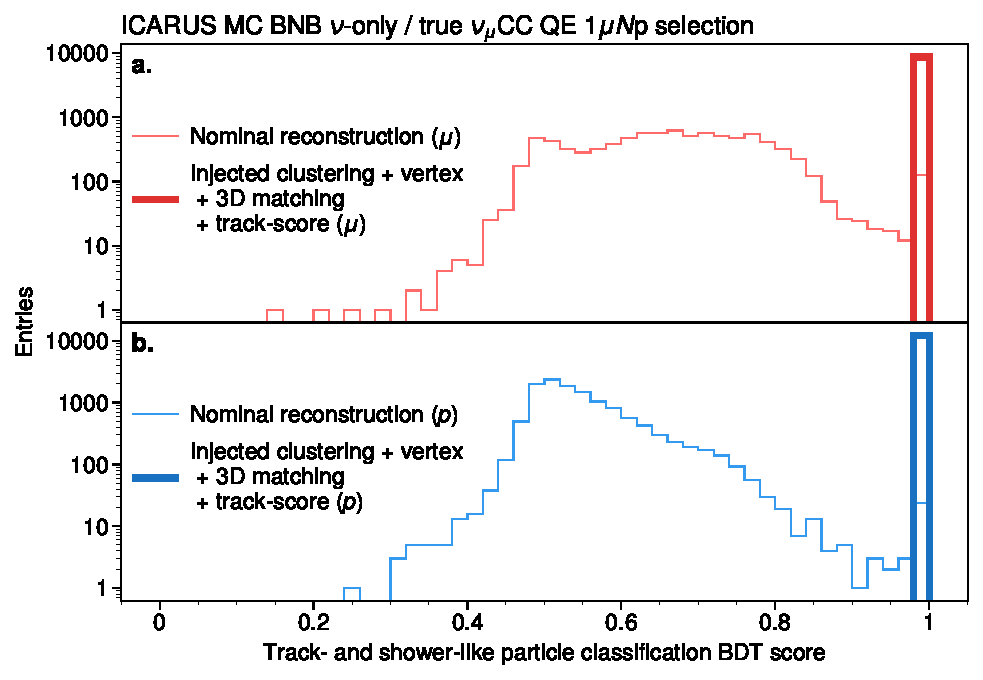
\includegraphics[width=0.95\linewidth]{pandora/chapter_4/toSlide_BDT_trackscore.pdf}
    \caption[Track and shower classification BDT score]{Plot of the score coming out of the track and shower BDT classification algorithm. Tracks have a score of 1, whereas showers have a score of 0. In the two panels there are muons (upper half, in red) and protons (lower half, in blue) with both the nominal reconstruction (thin line) as well as the cheated reconstruction and classification (thick line). }
    \label{fig:trackScoreCheated}
\end{figure}

Checking this stage downstream of the reconstruction is immediate by looking at the value of the BDT score in the particles that have a true label associated with muons and protons, or electrons and photons, that should be classified as tracks and electromagnetic showers, respectively. Tracks have a score of 1, whereas showers have a score of 0. \autoref{fig:trackScoreCheated} shows the assigned BDT score with the nominal (thin line) and cheated (thick line) particle classification stage for protons (blue) and muons (red). 

\subsection{Slice creation and tagging}

All these algorithms are part of the PandoraNeutrino reconstruction path, with both the 2D clustering and the 3D reconstruction stages also implemented in the PandoraFastReco and PandoraCosmic reconstruction paths. The PandoraFastReco is crucial, as part of the reconstruction chain, to perform a ``fast reconstruction'', allowing the slice creation tools to create the interaction slices. 

% why is slice creation core to the reconstruction?
Since this stage is run upstream of the PandoraNeutrino reconstruction path, ensuring a correct creation of the slices is core for the success of the subsequent reconstruction steps. As a matter of fact, if the slicing process fails and for some reason splits one interaction in half, the following reconstruction steps cannot recover the underlying interaction, even if cheating all the stages of the PandoraNeutrino reconstruction (i.e., making the reconstruction downstream of the slice creation ``perfect''). \autoref{fig:slicingIssue} shows this case with an example. In the figure, a $\PGnGm$CCQE Np event is shown. All the hits in the interaction are shown in the last panel. When the slice creation tool is run, however, it splits the prompt muon into two separate slices (Slice A/B, third and fourth panels). Then, performing the fully cheated reconstruction, thus effectively showing the underlying true particles in the interaction (Slice A/B, first two panels), reveals that what will be selected as a true and reconstructed $1\PGm1\Pp$ slice is Slice A. Slice B contains only half of the muon track and the muon decay Michel electron. 

%% issues (figure)
\begin{figure}[!htb]
    \centering
    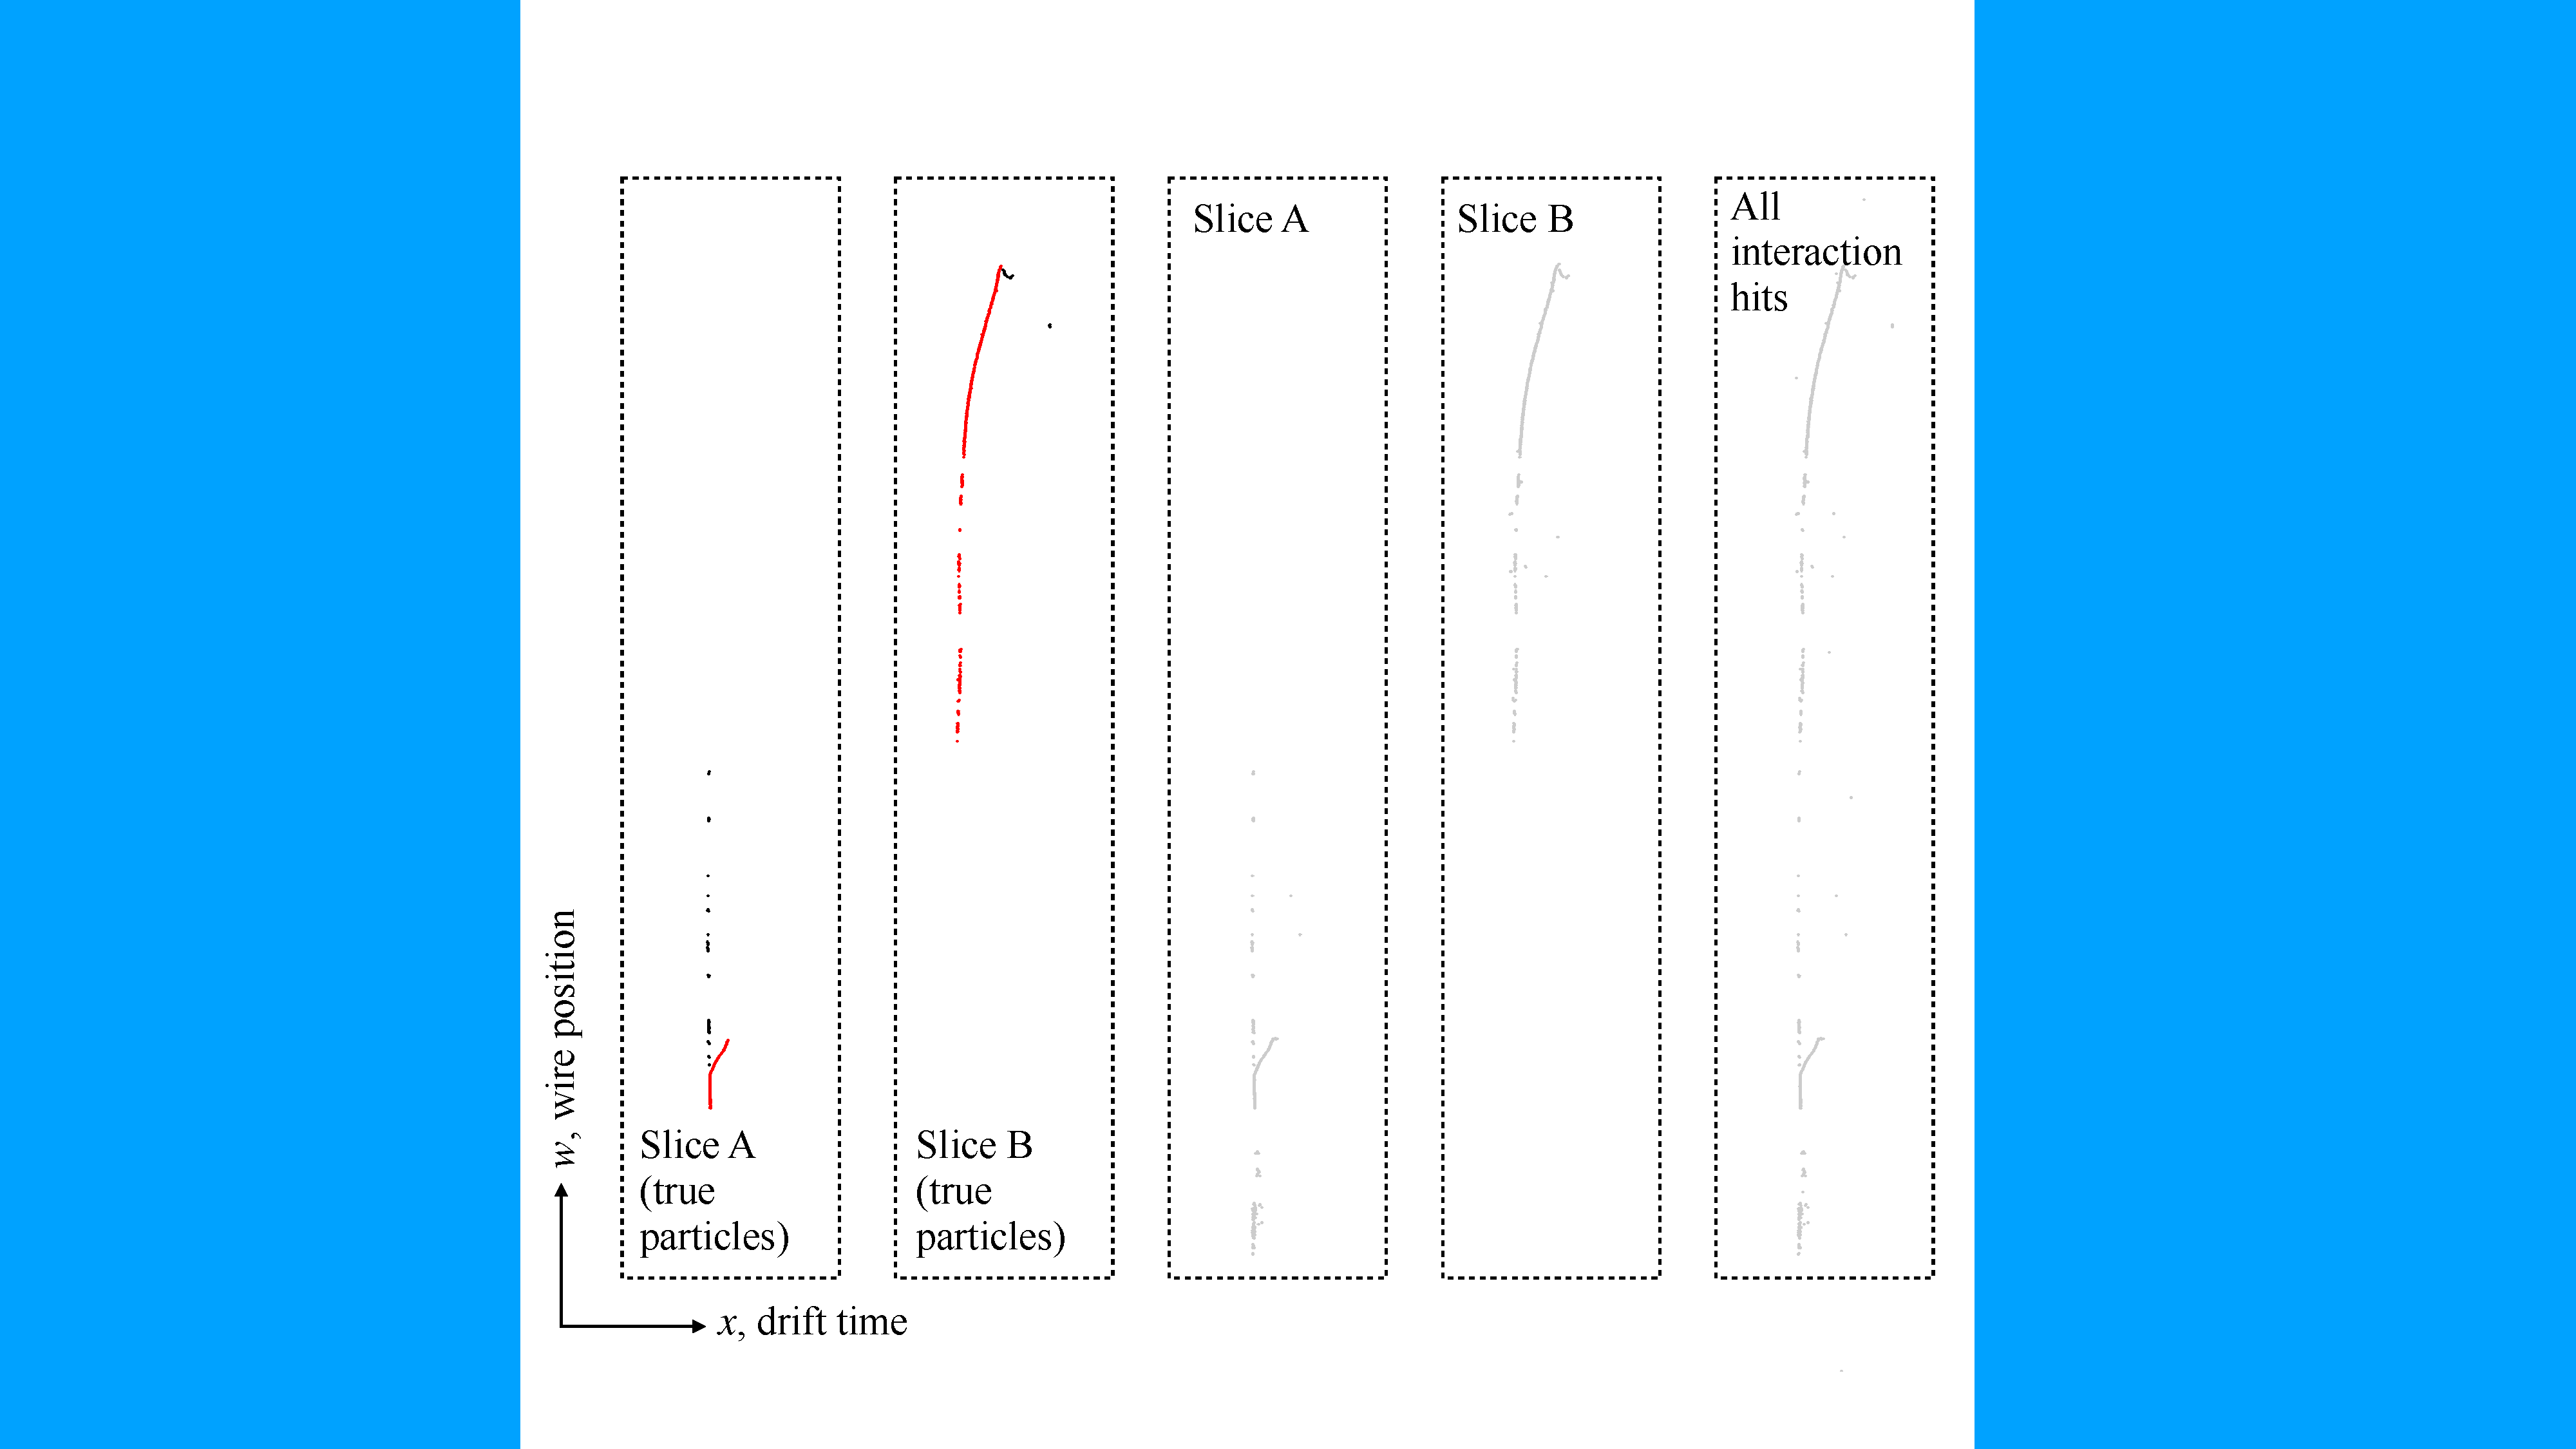
\includegraphics[width=0.95\linewidth, trim={14cm 0 16cm 0}, clip]{pandora/chapter_4/slicing.pdf}
    \caption[Slice creation failure mode]{Example of an event where the slice creation tool failed to correctly create one slice for the interaction, splitting it instead into two separate slices. }
    \label{fig:slicingIssue}
\end{figure}

% how this tool is implemented
Since discovering that this was not an isolated case, the cheating of the slice creation tool was also considered. The working principle of the cheated slice creation tool is pretty straightforward. This looks at all the reconstructed hits in the events and associates them with the correct MCParticles, which are arranged in the interaction with the correct hierarchy. Using the underlying MC information, this tool can therefore divide the hits on all three of the readout planes by the underlying interaction. These lists of hits divided by MC interaction are then used to have the downstream reconstruction performed on them. 


\section{Evaluating subsequent reconstruction stages}\label{sec:methods}

% aim of performing this analysis
Using this set of tools, whose performances have been thoroughly evaluated and whose limitations have been highlighted in the previous paragraphs, it is now possible to get a detailed understanding of where the reconstruction pipeline fails the most; therefore, provide a detailed path to what the problems are that should be addressed, weighing their relevance on the impact these changes can have on the reconstruction and downstream event selection performances. 

In order to achieve this, first the focus was moved to the PandoraNeutrino reconstruction path. Within this stage of the Pandora event reconstruction, five substages are identified: the 2D cluster creation, the 3D vertex creation, the 3D particle creation, the particle hierarchy creation, and the particle classification. As already addressed before, however, the particle hierarchy creation stage is delicate, and for this reason it is left out from this analysis. 

Having divided the PandoraNeutrino reconstruction into these five stages opened up the possibility of replacing any of them in the reconstruction with their cheated version. The idea is to create five reconstruction chains that process the same events. Each one differs from the previous by one stage that is cheated in the former and kept nominal in the latter. Starting from a fully cheated configuration, where the 2D cluster creation, the 3D vertex creation, the 3D particle creation, and the particle classification are cheated, replacing the last with its nominal configuration leaves only the 2D cluster creation, the 3D vertex creation, and the 3D particle creation cheated. Continuing on with the same idea for all the stages in the PandoraNeutrino reconstruction, with the exception of the particle hierarchy creation algorithm, the last configuration has all the stages in their nominal format. 

% method
Under the assumption that the Pandora reconstruction algorithms are decoupled from one another (see \autoref{sec:TPC_reco_gen} and the references therein), it is possible to say that the reconstruction and event selection efficiency is the result of the product of the efficiency of the signal processing stage (its efficiency in reconstructing the hits on the readout planes) with the efficiencies of the individual steps of the event reconstruction and the event selection efficiency, provided the event reconstruction, \begin{equation}
    \begin{aligned}
        \epsilon &= 
        \epsilon_\mathrm{signal\ processing} \times 
        \epsilon_\mathrm{2D\ clusters} \times 
        \epsilon_\mathrm{vertex\ creation} \times \\
        &\quad\quad\quad\times
        \epsilon_\mathrm{3D\ reconstruction} \times 
        \epsilon_\mathrm{particle\ classification} \times 
        \epsilon_\mathrm{event\ selection}
    \end{aligned}\label{eq:componentsEfficiency}
\end{equation} 

Making the reasoned assumption that cheating a step of the reconstruction makes its efficiency effectively \SI{100}{\percent}, and indicating with an asterisk the efficiency of a cheated stage of the reconstruction, it is possible to compare two of the aforementioned configurations that differ only for the cheating of a single step. For example, the ratio between the efficiencies of the ``fully cheated'' configuration (A) and the ``cheated up to the particle classification algorithm'' configuration (B) is \begin{equation}
    \frac{
    \epsilon^\mathrm{B}
    }{
    \epsilon^\mathrm{A}
    } = \frac{
    \epsilon_\mathrm{sig.} \times 
    \epsilon_\mathrm{2D}^* \times 
    \epsilon_\mathrm{vertex}^* \times 
    \epsilon_\mathrm{3D}^* \times 
    \epsilon_\mathrm{class.} \times 
    \epsilon_\mathrm{ev.\ sel.}^\mathrm{B}
    }{
    \epsilon_\mathrm{sig.} \times 
    \epsilon_\mathrm{2D}^* \times 
    \epsilon_\mathrm{vertex}^* \times 
    \epsilon_\mathrm{3D}^* \times 
    \epsilon_\mathrm{class.}^* \times 
    \epsilon_\mathrm{ev.\ sel.}^\mathrm{A}
    } = \frac{
    \epsilon_\mathrm{class.}
    }{
    \epsilon_\mathrm{class.}^*
    } \times \qty(\frac{
    \epsilon_\mathrm{ev.\ sel.}^\mathrm{B}
    }{
    \epsilon_\mathrm{ev.\ sel.}^\mathrm{A}
    }) \label{eq:methodBase}
\end{equation} Here the apex refers to which of the configurations is used, except for the asterisks mentioned before. The configurations are presented in \autoref{tab:configurations}, and the configuration Id. is used within the equations. Additionally, the notation is simplified to allow for ease. 

\begin{table}[]
    \centering
    \caption[List of configurations]{List of all the configurations used for the evaluation of the reconstruction performances in \autoref{sec:methods}. The red cross mark {\tikzxmark} indicates the steps of the reconstruction that are kept nominal, whereas the green tick mark {\tikzcmark} indicates those that are cheated. }
    \label{tab:configurations}
    \small
    \begin{tabular}{lp{4cm}cccc}
        \hline
         & & 2D clusters & Vertex & 3D particles & Particles \\
         Id. & Configuration name & creation & creation & reconstruction & classification \\
         \hline
         A & Fully cheated & \tikzcmark & \tikzcmark & \tikzcmark & \tikzcmark \\
         B & Cheated up to the particle classification algorithm & \tikzcmark & \tikzcmark & \tikzcmark & \tikzxmark \\
         C & Cheated up to the particle three-dimensional reconstruction algorithm & \tikzcmark & \tikzcmark & \tikzxmark & \tikzxmark \\
         D & Cheated up to the vertex reconstruction & \tikzcmark & \tikzxmark & \tikzxmark & \tikzxmark \\
         E & Nominal & \tikzxmark & \tikzxmark & \tikzxmark & \tikzxmark \\
         \hline
    \end{tabular}
\end{table}

In Eq. \eqref{eq:methodBase} all the common terms in the ratio ($\epsilon_\mathrm{sig.}, \epsilon_\mathrm{2D}^*, \epsilon_\mathrm{vertex}^*, \epsilon_\mathrm{3D}^*$) are cancelled. 

Developing Eq. \eqref{eq:methodBase} further, it is possible to get a value that is proportional to the efficiency of the particle classification algorithm, \begin{equation}
    \epsilon_\mathrm{class.} \times \qty(\frac{
    \epsilon_\mathrm{ev.\ sel.}^\mathrm{B}
    }{
    \epsilon_\mathrm{ev.\ sel.}^\mathrm{A}
    }) = \frac{
    \epsilon^\mathrm{B}
    }{
    \epsilon^\mathrm{A}
    } \times \epsilon_\mathrm{class.}^* \label{eq:stageEfficiencyPrePID_0}
\end{equation} It is worth noting that, under the reasoned assumption that $\epsilon_\mathbf{any\ single\ stage}^* = \SI{100}{\percent}$, we can actually drop this term in Eq. \eqref{eq:stageEfficiencyPrePID_0}, thus have \begin{equation}
    \epsilon_\mathrm{class.} \times \qty(\frac{
    \epsilon_\mathrm{ev.\ sel.}^\mathrm{B}
    }{
    \epsilon_\mathrm{ev.\ sel.}^\mathrm{A}
    }) = \frac{
    \epsilon^\mathrm{B}
    }{
    \epsilon^\mathrm{A}
    } \label{eq:stageEfficiencyPrePID}
\end{equation}

\subsection{Results} \label{sec:resultsLadder}

%% evaluation of the erformances
%% step by step issues (if any)
Having established the analysis method, the first operation was to compute the reconstruction and selection efficiency for all the configurations shown in \autoref{tab:configurations}. To perform a preliminary analysis, the integrated efficiency was computed: looking at the total count of true and reconstructed neutrinos over the total number of true neutrino $\PGnGm$CCQE Np  interactions. These efficiencies are compared in \autoref{fig:efficiencyNoNu}. A first remark that can be made is that, as more steps of the reconstruction are cheated, the overall efficiency increases: this suggests that, at least, the addition of any cheated algorithm improves the event reconstruction. A second remark can be made by just visually analysing the different efficiencies achieved by the different configurations. For example, it is clear that once the 2D clusters are created correctly, i.e., cheated, the reconstruction performs better overall by comparing the nominal reconstruction (configuration E) with the ``injected clustering'' (configuration D) bin, \SI{54.7(5)}{\percent} and \SI{63.1(5)}{\percent} respectively. This information tells us the impact of the cluster creation algorithms is high. The same can be said for the difference between the ``injected cluster'' (configuration D) and the ``injected cluster + vertex'' (configuration C) bins, \SI{63.1(5)}{\percent} and \SI{68.1(5)}{\percent} respectively: the vertex creation algorithm has a great impact, and there is a large overhead in terms of improvements that can be achieved. 

\begin{figure}
    \centering
    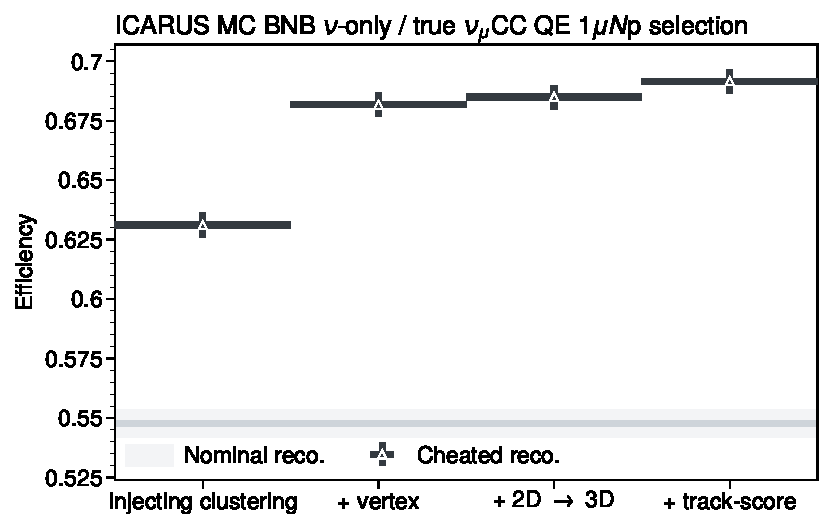
\includegraphics[width=0.85\linewidth]{pandora/chapter_4/CCNp_efficiencyNoNu.pdf}
    \caption[Evaluation of the reconstruction and selection efficiency for different configurations]{Evaluation of the event reconstruction and selection efficiencies for the configuration presented in \autoref{tab:configurations}. Each bin label shows which are the cheated stages, the first having only the clustering creation cheated (configuration D), each time adding a cheated step up to the fully cheated configuration A in the last bin. }
    \label{fig:efficiencyNoNu}
\end{figure}

% results
We can now exploit these results to compute a value which is proportional to the efficiency of each reconstruction step, factorising the event selection efficiency for the two configurations considered in the computation; see Eq. \eqref{eq:stageEfficiencyPrePID}. Running the computations for all possible combination of subsequent configurations, we can extract the values proportional to the single-stage efficiencies, \begin{align}
    \epsilon_\mathrm{2D\ clusters} \times 
    \qty(\frac{\epsilon_\mathrm{ev.\ sel.}^\mathrm{E}}{\epsilon_\mathrm{ev.\ sel.}^\mathrm{D}}) 
    &= \frac{\epsilon^\mathrm{E}}{\epsilon^\mathrm{D}} = \frac{\SI{54.7(5)}{\percent}}{\SI{63.1(5)}{\percent}} = 
    \SI[round-mode = uncertainty]{86.779059+-1.104354}{\percent} \\
    \epsilon_\mathrm{vertex\ creation} 
    \times \qty(\frac{\epsilon_\mathrm{ev.\ sel.}^\mathrm{D}}{\epsilon_\mathrm{ev.\ sel.}^\mathrm{C}}) 
    &= \frac{\epsilon^\mathrm{D}}{\epsilon^\mathrm{C}} = \frac{\SI{63.1(5)}{\percent}}{\SI{68.1(5)}{\percent}} = 
    \SI[round-mode = uncertainty]{92.575370+-1.024352}{\percent} \\
    \epsilon_\mathrm{3d\ reconstruction} 
    \times \qty(\frac{\epsilon_\mathrm{ev.\ sel.}^\mathrm{C}}{\epsilon_\mathrm{ev.\ sel.}^\mathrm{B}}) 
    &= \frac{\epsilon^\mathrm{C}}{\epsilon^\mathrm{B}} = \frac{\SI{68.1(5)}{\percent}}{\SI{68.4(5)}{\percent}} = 
    \SI[round-mode = uncertainty]{99.526687+-1.041368}{\percent} \\
    \epsilon_\mathrm{particle\ classification} 
    \times \qty(\frac{\epsilon_\mathrm{ev.\ sel.}^\mathrm{B}}{\epsilon_\mathrm{ev.\ sel.}^\mathrm{A}}) 
    &= \frac{\epsilon^\mathrm{B}}{\epsilon^\mathrm{A}} = \frac{\SI{68.4(5)}{\percent}}{\SI{69.1(5)}{\percent}} = 
    \SI[round-mode = uncertainty]{99.039894+-1.024644}{\percent}
\end{align}

It would be sensible to make the educated guess that the selection efficiencies are not drastically different; therefore, it is sensible to assume that the ratios between the selection efficiencies in the two configurations for each pair are close to unity. However, this is a qualitative assumption. To make this quantitative, it would be necessary to constrain the selection efficiency.

For this reason, it is interesting to take a detour and look at the impact of cheating the reconstruction on each selection cut. To do so, the event reconstruction and selection efficiency are computed each time, changing the reconstructed signal definition by cumulatively adding selection cuts. \autoref{fig:efficiencyByCut} is the result of computing this cut-by-cut efficiency for all five configurations in \autoref{tab:configurations}. 

\begin{figure}
    \centering
    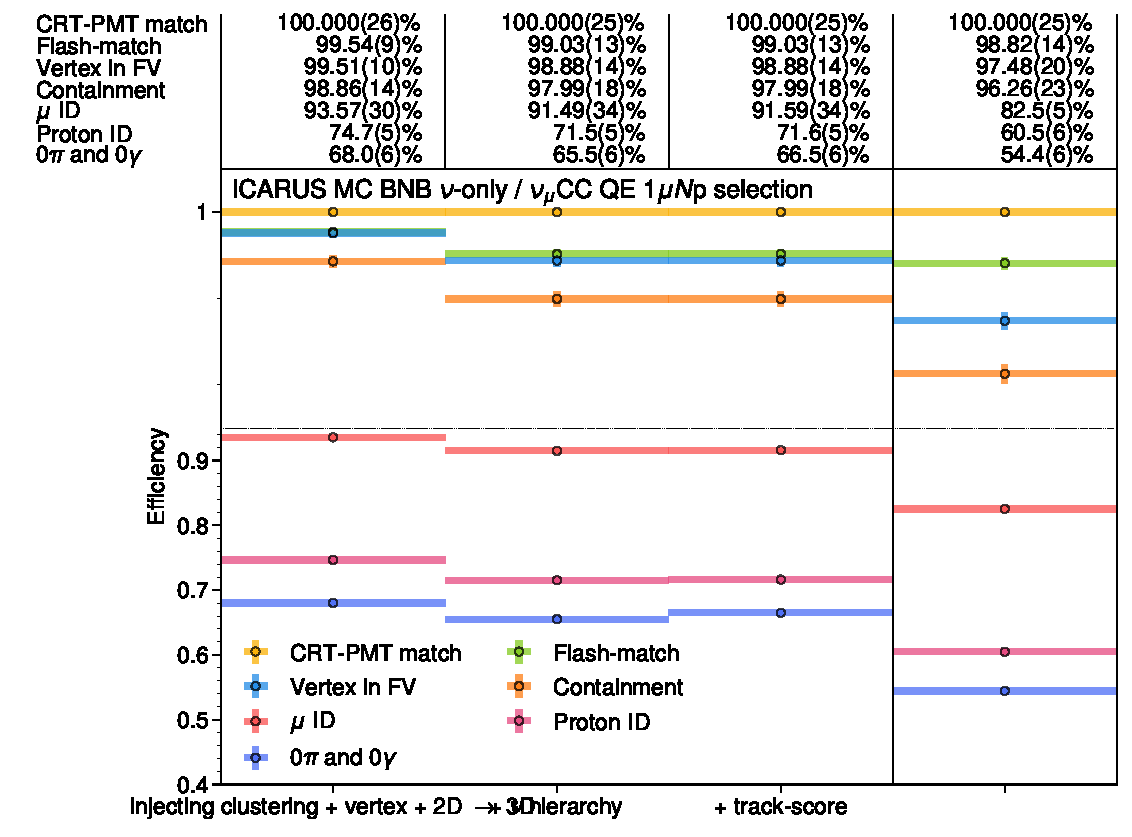
\includegraphics[height=9cm]{thesis/6_figures/pandora/chapter_4/CCNp_efficiencyByCut_noNu_cheatingSlice.pdf}
    \caption[Event reconstruction and selection efficiency for different cuts]{Cut-by-cut event reconstruction and selection efficiency for all configurations in \autoref{tab:configurations}. Each time a selection cut is added to the list. The top table shows the efficiency of each configuration for each selection cut. It is worth remarking that the scale on the $y$ axis is not uniform, but the region from 0.9 to 1 is scaled up to allow for better visual separation of the cuts. }
    \label{fig:efficiencyByCut}
\end{figure}

% \cleardoublepage
% !TEX root=../main.tex

\subsection{Extracting the selection efficiency} \label{sec:efficiencyPidExtraction}

Referring to \autoref{fig:efficiencyByCut} it is evident that the first selection cut, i.e. CRT-PMT matching, has no impact on the events.
For the present study, this is due to the type of events analysed, that include only neutrino candidate interactions, i.e. neither in-time nor out-of-time cosmics are simulated.
The second cut, Flash-match, has a very small effect: this has the same explanation as CRT-PMT cut, since no cosmic-ray interaction is generated for the presently used sample.
The first cut that introduces a reduction in the selected statistics is the requirement on the vertex position to lie inside the fiducial volume of the detector.
This is a request that is strongly dependent on the reconstruction performance; therefore, it is expected that an improved vertex reconstruction results in an overall improvement on the efficiency.
The following request that all particles are contained in the active volume of the detector is also strongly dependent on the reconstruction performance. Correct clustering of the hits and start-/end-point assignation is correlated with containment (if the true particles are contained, so should be the reconstructed ones). 
The last selection cuts concern the muon and proton identifications and the no-charged-pion and no-electromagnetic-shower requests. These have a large impact on the event selection efficiency, with a ${\sim}\SI{15}{\percent}$ loss in the identification of the proton, followed by the ${\sim}\SI{5}{\percent}$ loss due to the identification and rejection of charged pions and electromagnetic showers. The particle identification cuts, described in detail in \autoref{sec:dataSample_and_selection}, follows from cuts on variables that are direct consequence of the efficiency of Pandora reconstruction, such as the length requirements, the track and shower classification BDT score, the distance from the interaction vertex, and the particle hierarchy requirements, as well as variables that are heavily influeced by the calorimentric reconstruction performances, downstream of Pandora event reconstruction (see \autoref{sec:calorimetryAndCalibration}). Assuming the correlation between variables that depend on Pandora topological reconstruction quality and variables that depends on the calorimetric reconstruction effectiveness is small, it is possible to factorise their contribution to the final selection efficiency, assigning a ``reconstruction-related'' event selection efficiency to the former and a ``PID-related'' event selection efficiency to the latter, \begin{equation}
    \epsilon_\mathrm{event\ selection} = \epsilon_\mathrm{ev.\ sel.,\ reco.} \times \epsilon_\mathrm{ev.\ sel.,\ pid}. \label{eq:originalSelEfficiency}
\end{equation} 

Considering Eq. \eqref{eq:componentsEfficiency}, we can rewrite it, as \begin{equation}
    \begin{aligned}
        \epsilon &= 
        \epsilon_\mathrm{signal\ processing} \times 
        \epsilon_\mathrm{2D\ clusters} \times 
        \epsilon_\mathrm{vertex\ creation} \times 
        \epsilon_\mathrm{3D\ reconstruction} \times \\
        &\quad\quad\quad\times
        \epsilon_\mathrm{particle\ classification} \times 
        \epsilon_\mathrm{event\ selection,\ reco.} \times 
        \epsilon_\mathrm{event\ selection,\ pid}.
    \end{aligned} \label{eq:componentsEfficiencyPid}
\end{equation} We can make an additional assumption.
Since the term $\epsilon_\mathrm{event\ selection,\ reco.}$ is related to the reconstruction efficiency, it is reasonable to assume that each stage in the reconstruction chain will give its specific contribution to the overall value.
This hypothesis is supported, for example, by the observation that once the vertex reconstruction is cheated, the requirement that the vertex lie inside the TPC fiducial volume is automatically satisfied, as can be seen in \autoref{fig:efficiencyByCut}. In other words, the component of the selection efficiency associated with vertex containment is correlated with the success of correctly assigning the true interaction vertex. Taking this into account, we can rewrite Eq. \eqref{eq:componentsEfficiencyPid} as \begin{equation}
    \begin{aligned}
        \epsilon &= 
        \epsilon_\mathrm{signal\ processing} \times 
        \epsilon_\mathrm{2D\ clusters}' \times 
        \epsilon_\mathrm{vertex\ creation}' \times 
        \epsilon_\mathrm{3D\ reconstruction}' \times \\
        &\quad\quad\quad\times
        \epsilon_\mathrm{particle\ classification}' \times 
        % \epsilon_\mathrm{event\ selection,\ reco.} \times 
        \epsilon_\mathrm{ev.\ sel.,\ pid}
        = 
        \epsilon_\mathrm{sig.\ proc.} \times 
        \epsilon_\mathrm{reco.}' \times 
        \epsilon_\mathrm{ev.\ sel.,\ pid},
    \end{aligned} \label{eq:componentsEfficiencyPidNew}
\end{equation} where the prime symbol $'$ is added to highlight that the efficiencies listed here slightly differ from the ones above in Eq. \eqref{eq:componentsEfficiencyPid}. Following the same strategy outlined in Eq. \eqref{eq:componentsEfficiency}--\eqref{eq:stageEfficiencyPrePID}, we now obtain a new version of \begin{equation}
    \epsilon_\mathrm{particle\ class.} \times \qty(\frac{
    \epsilon_\mathrm{ev.\ sel., pid}^\mathrm{B}
    }{
    \epsilon_\mathrm{ev.\ sel., pid}^\mathrm{A}
    }) = \frac{
    \epsilon^\mathrm{B}
    }{
    \epsilon^\mathrm{A}
    }. 
\end{equation} where we dropped the prime symbol for simplicity. We can now invert the equation to extract the term we want to evaluate: \begin{equation}
    \epsilon_\mathrm{particle\ class.} = \frac{
    \epsilon^\mathrm{B}
    }{
    \epsilon^\mathrm{A}
    } \times \frac{
    \epsilon_\mathrm{ev.\ sel., pid}^\mathrm{A}
    }{
    \epsilon_\mathrm{ev.\ sel., pid}^\mathrm{B}
    }, \label{eq:stageEfficiencyPostPID}
\end{equation} It is clear that to do this we need a final ingredient, which is given by the impact of PID onto selection efficiency, i.e.,  $\epsilon_\mathrm{ev.\ sel.,\ pid}$. To extract such a parameter, we developed a modified event selection that allowed the effects of particle identification to be decoupled from the effects of the event reconstruction. In this modified event selection, all the cuts performed on variables that depend on the reconstruction performance are left unaltered, whereas the cuts that are dependent on the calorimetric particle identification are effectively bypassed considering the true particle labels. The requirements for this ``modified'' particle identification are detailed below.  

\noindent
To identify if a single muon is present in the interaction, the following cuts are applied: \begin{itemize}
    \item the particle should be tagged as a primary particle by Pandora,
    \item the conversion gap should be smaller than \SI{10}{\cm},
    \item the track/shower classification score should be greater than 0.5,
    \item the track length should be greater than \SI{50}{\cm},
    \item the label assigned via match with Monte Carlo information should correspond to a muon. 
\end{itemize}
For the protons in the interaction, the following cuts are applied: \begin{itemize}
    \item the particle should be tagged as a primary particle by Pandora,
    \item the conversion gap should be smaller than \SI{10}{\cm},
    \item the track/shower classification score should be greater than 0.4,
    \item the reconstructed deposited energy and the true kinetic energy should be greater than \SI{50}{\MeV},
    \item the label assigned via match with Monte Carlo information should correspond to a proton.
\end{itemize}
For pions, the selection is the same as for protons, with the sole difference of requiring the true label of a charged pion and a lower energy threshold of \SI{25}{\MeV}. 

\noindent
For electromagnetic showers, the following cuts are applied: \begin{itemize}
    \item the particle should be tagged as a primary particle by Pandora,
    \item the track/shower classification score should be smaller than 0.5,
    \item the reconstructed deposited energy and the true kinetic energy should be greater than \SI{25}{\MeV},
    \item the label assigned via match with Monte Carlo information should correspond to an electron or a photon. 
\end{itemize} 


Using this modified event selection, we extract again the efficiencies as a function of cheated stages and selection cuts (see \autoref{fig:efficiencyNoNu}). \autoref{fig:CCNp_efficiencyNoNu_cheatingPid} shows the efficiency for the same configurations (see \autoref{tab:configurations}) with the modified event selection. 

\begin{figure}
    \centering
    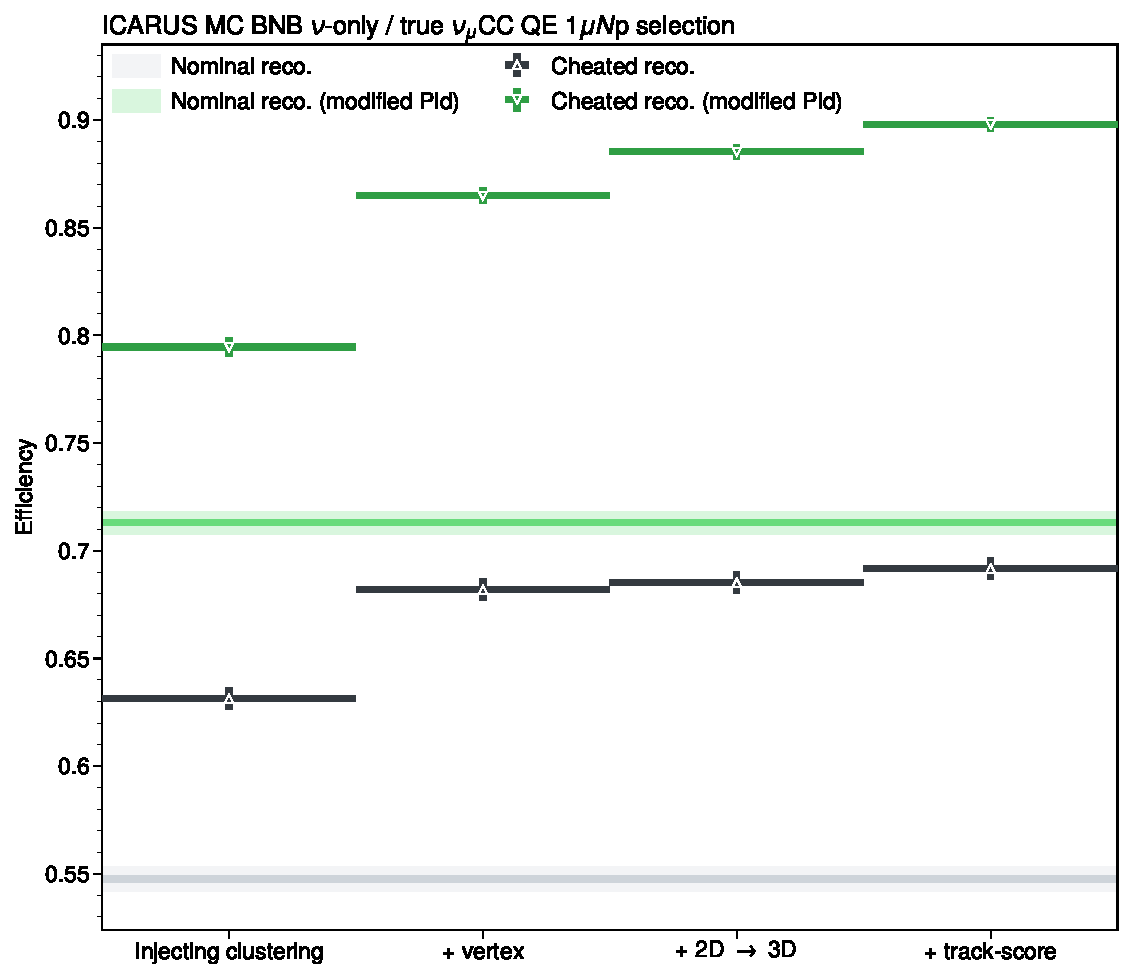
\includegraphics[width=0.85\linewidth]{pandora/chapter_4/CCNp_efficiencyNoNu_cheatingPid.pdf}
    \caption[Evaluation of the reconstruction and selection efficiency for different configurations with the modified event selection]{Evaluation of the event reconstruction and selection efficiency for all the configurations listed in \autoref{tab:configurations}. Both the event selection with the nominal particle identification (black markers) and the event selection with the modified particle identification (green markers) are shown. }
    \label{fig:CCNp_efficiencyNoNu_cheatingPid}
\end{figure}

% Extracting the efficiency here
For this modified event selection we can assume that the overall efficiency that accounts both for reconstruction, PID and selection is \begin{equation}
    \epsilon^\mathrm{mod.\ selection} = \epsilon_\mathrm{sig.\ proc.} \times 
        \epsilon_\mathrm{reco.} \times 
        \epsilon_\mathrm{ev.\ sel.,\ pid}^\mathrm{mod.\ selection}. 
        \label{eq:modifiedPidEfficiency}
\end{equation} This modified event selection does not rely on the performance of the PID, using the true underlying MC label to uniquely identify reconstructed particle species. Therefore we assumed that  $\epsilon_\mathrm{ev.\ sel.,\ pid}^\mathrm{mod.\ selection}\simeq1$, since no particle misidentification inefficiencies related to PID are possible. We exploit this simplification, and comparing Eq. \eqref{eq:modifiedPidEfficiency} and \eqref{eq:componentsEfficiencyPidNew}, we can extract the efficiency of the particle identification stage for each configuration of \autoref{tab:configurations}. The ratio of these two equations leads to \begin{equation}
    \frac{
    \epsilon^{\mathrm{mod.\ selection,}\ c}
    }{
    \epsilon^{c}
    } = \frac{
    \epsilon_\mathrm{sig.\ proc.} \times 
    \epsilon_\mathrm{reco.} \times 
    \epsilon_\mathrm{ev.\ sel.,\ pid}^{\mathrm{mod.\ selection,}\ c}
    }{
    \epsilon_\mathrm{sig.\ proc.} \times 
    \epsilon_\mathrm{reco.} \times 
    \epsilon_\mathrm{ev.\ sel.,\ pid}^c
    } = \frac1{\epsilon_\mathrm{ev.\ sel.,\ pid}^c} \label{eq:tmpEq20}
\end{equation} for each configuration $c$. By inverting Eq. \eqref{eq:tmpEq20} we can estimate the contribution of particle identification, and thus calorimetric reconstruction, to the overall selection efficiency. \begin{equation}
    \epsilon_\mathrm{ev.\ sel.,\ pid}^c = \frac{
    \epsilon^{c}
    }{
    \epsilon^{\mathrm{mod.\ selection,}\ c}
    }. \label{eq:pidComputation}
\end{equation} The particle identification efficiencies extracted are reported in \autoref{tab:pidEfficiencyPerConfiguration}. 

\begin{table}[]
    \centering
    \caption[Particle identification efficiency for all configurations]{For each configuration the corresponding efficiency is shown, using both the nominal event selection and the modified event selection described in \autoref{sec:efficiencyPidExtraction}. The third column is the resulting efficiency of the particle identification step.  Further details on the evaluation of the listed parameters are provided in the text.}
    \label{tab:pidEfficiencyPerConfiguration}
    \begin{tabular}{lp{3.5cm}ccc}
        \hline
         Id. & Configuration name & $\epsilon$ & $\epsilon^\mathrm{mod.\ selection}$ & $\epsilon_\mathrm{ev.\ sel.,\ pid}$ \\
         & & (see Eq. \ref{eq:originalSelEfficiency}) & (see Eq. \ref{eq:modifiedPidEfficiency}) & (see Eq. \ref{eq:pidComputation})\\ 
         \hline
         A & Fully cheated & \SI{69.2(5)}{\percent} & \SI{89.78(33)}{\percent} & \SI{77.1(6)}{\percent} \\
         B & Cheated up to the particle classification algorithm & \SI{68.5(5)}{\percent} & \SI{88.52(35)}{\percent} & \SI{77.4(6)}{\percent} \\
         C & Cheated up to the particle three-dimensional reconstruction algorithm & \SI{68.2(5)}{\percent} & \SI{86.5(4)}{\percent} & \SI{78.8(7)}{\percent} \\
         D & Cheated up to the vertex reconstruction & \SI{63.1(5)}{\percent} & \SI{79.5(4)}{\percent} & \SI{79.4(8)}{\percent} \\
         E & Nominal & \SI{54.8(5)}{\percent} & \SI{71.3(5)}{\percent} & \SI{76.8(9)}{\percent} \\
         \hline
    \end{tabular}
\end{table}

By replacing the PID efficiency values extracted thanks to the modified selection in Eq. \eqref{eq:stageEfficiencyPostPID}, we can derive an estimate for the efficiency of each stage of the reconstruction. This leads to the following results \begin{equation}
    \begin{aligned}
        \epsilon_\mathrm{reco.} =&\
        \epsilon_\mathrm{2D\ clusters} &\times&\ 
        \epsilon_\mathrm{vertex\ creation} &\times&\ 
        \epsilon_\mathrm{3D\ reco.} &\times&\ 
        \epsilon_\mathrm{particle\ class.} =\\  
        =&\ \SI{89.7(1.8)}{\percent} &\times&\ 
        \SI{91.9(1.6)}{\percent} &\times&\ 
        \SI{97.7(1.6)}{\percent} &\times&\ 
        \SI{98.6(1.5)}{\percent}
    \end{aligned}\label{eq:results}
\end{equation}

These findings should be interpreted with caution. Firstly, they are obtained targeting a specific event topology. Therefore, it is reasonable to assume that a different event topology would yield significantly different results. As explicitly stated throughout the text, numerous assumptions and approximations have been made to obtain these results. All correlations between the various algorithms involved in Pandora reconstruction chain are assumed to be minimal. Additionally, to obtain the selection efficiencies, most of the variables involved in the event selection cuts are assumed to be uncorrelated. These assumptions hold true to a certain extent. 

However, as discussed in the subsequent section, an independent test on the vertex reconstruction was conducted. The results from this independent test, which are in good agreement with the results in Eq. \eqref{eq:results}, suggest that the starting point hypothesis is reasonable. 
% \cleardoublepage

\section{Impact of the vertex reconstruction} \label{sec:vertexResults}

% from previous ... the vertex is quite relevant
From the results shown in \autoref{sec:resultsLadder} and \autoref{sec:efficiencyPidExtraction} it is possible to deduce that assigning correctly the interaction vertex plays a central role in the event reconstruction. This is obviously true for electromagnetic showers, where the distance from the vertex, often referred to as the ``conversion gap'', is key to classifying electron-induced electromagnetic showers from photon-induced ones. Since the radiation length $X_0$ in LAr is approximately \SI{14}{\cm}, having an accurate measurement of the vertex location, with a $\mathcal{O}(\si{\mm})$ precision, is core for future studies. Moreover, it was shown, in previous sections, that there are cases also where, for simpler topologies (such as the $\PGnGm$CC QE Np topologies), improving the vertex results in an overall improvement of the reconstruction. 

% since its "uncorrelated" and do not depend on the previous step success that much, cheat it alone
Since the vertex reconstruction, differently from other stages in the PandoraNeutrino reconstruction path, is truly disentangled from the other steps, it is also sensible to study the effects of cheating it alone. \autoref{fig:cheatedVertexByCut} shows the impact of cheating the vertex reconstruction, in terms of efficiency, considering each cut of the event selection alone. There are multiple elements in the plot in \autoref{fig:cheatedVertexByCut}. The three bins are the three used configurations, which are also shown in \autoref{tab:configurationsVertexCheating}. As mentioned in \autoref{tab:configurationsVertexCheating}, the ``Inj. vertex selection'' configuration is cheating only the vertex selection, i.e., replacing the BDT algorithm that selects the best interaction vertex from the list of the candidate vertices. 

\begin{figure}[!htb]
    \centering
    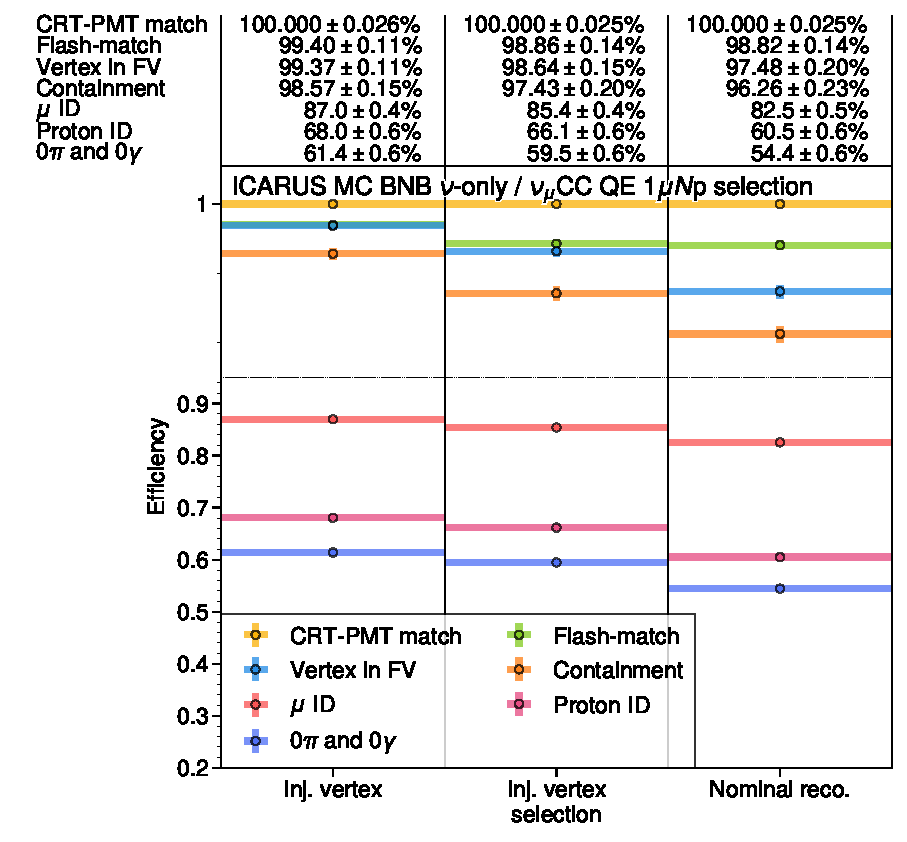
\includegraphics[height=9cm]{pandora/chapter_4/CCNp_efficiencyByCut_singles_2d_vtx_only.pdf}
    \caption[Event reconstruction and selection efficiency with the cheated vertex creation]{Cut-by-cut event reconstruction and selection efficiency for all configurations in \autoref{tab:configurationsVertexCheating}. Each time a selection cut is added to the list. The top table shows the efficiency of each configuration for each selection cut. It is worth remarking that the scale on the $y$ axis is not uniform, but the region from 0.9 to 1 is scaled up to allow for better visual separation of the cuts. }
    \label{fig:cheatedVertexByCut}
\end{figure}

\begin{table}[]
    \centering
    \caption[List of configurations (vertex cheating)]{List of all the configurations used for the evaluation of the reconstruction performances in \autoref{sec:vertexResults}. The red cross mark {\tikzxmark} indicates the steps of the reconstruction that are kept nominal, whereas the green tick mark {\tikzcmark} indicates those that are cheated. The orange asterisk {\tikzsmark} indicates that the cheating is done partially, such as in the case of the CheatedVertexSelection algorithm. }
    \label{tab:configurationsVertexCheating}
    \small
    \begin{tabular}{lp{4cm}cccc}
        \hline
         & & 2D clusters & Vertex & 3D particles & Particles \\
         Id. & Configuration name & creation & creation & reconstruction & classification \\
         \hline
         A & Cheated vertex creation algorithm (Inj. vertex) & \tikzxmark & \tikzcmark & \tikzxmark & \tikzxmark \\
         B & Cheated vertex selection algorithm (Inj. vertex selection) & \tikzxmark & \tikzsmark & \tikzxmark & \tikzxmark \\
         C & Nominal & \tikzxmark & \tikzxmark & \tikzxmark & \tikzxmark \\
         \hline
    \end{tabular}
\end{table}

% results in terms of efficiency
% how this impacts other variables (i.e. is this impacting the selection eff or just the reconstruction eff... of 1µNp events?)
Looking at the result, a similar pattern to that of the previous section is present: improving the reconstruction of the vertex does boost the event reconstruction performances. The efficiencies shown in \autoref{fig:cheatedVertexByCut}, especially the efficiency obtained when adding all selection cuts, provide a quantitative upper limit on the boost one might expect if the vertex reconstruction is improved. Having established that there is enough overhead to improve the vertex reconstruction, A and B configurations in \autoref{tab:configurationsVertexCheating} provide, however, different insight on the event reconstruction performances. 

In configuration B only the vertex selection step is cheated, meaning that the creation of the vertex candidates is still performed by the nominal reconstruction, but only the vertex closest in space to the true one gets selected. This configuration provides an understanding of how much it is possible to improve the algorithm that performs the vertex selection: it is essentially saying that, if the vertex selection process were perfect, the improvement in terms of event reconstruction and selection efficiency would be so much. The results in \autoref{fig:CheatingVertexCreation} show that when cheating the vertex selection, an improvement from the nominal reconstruction and selection efficiency ($\epsilon = \SI{54.4(6)}{\percent}$) of \SI{5.1(8)}{\percent} is achieved. 

Looking at this result, one might conclude that the next step in improving reconstruction efficiency should be to improve the algorithm responsible for selecting the correct interaction vertex. In the ideal case, this would lead to an enhancement in terms of downstream efficiency of about \SI{5}{\percent}. However, before rushing into conclusions, it is sensible to delve into the results obtained with the other configuration. 

Looking at the results from configuration A, it is possible to answer the question <<How would the reconstruction efficiency improve if the vertex were reconstructed and assigned correctly all the time?>>, provided that there is a way to assess that little-to-no impact on the efficiency increase comes from the particle identification. For this reason it  is useful to look, for example, at the distribution of the PID score. These are in \autoref{fig:chi2_cheatedVertex}. Looking at the distribution, and also at the cheated-over-nominal ratio, it is possible to deduce that the hypothesis that cheating the vertex creation does not alter in a significant way the Pid score of the selected particles can be considered acceptable. Thereafter, it is possible to conclude that the $\SI{7.0(8)}{\percent}$ maximum improvement, going from the nominal reconstruction efficiency ($\SI{54.4(6)}{\percent}$) to the reconstruction efficiency for the configuration where the vertex creation is cheated ($\SI{61.4(6)}{\percent}$), is predominately due to improvements in the event reconstruction following the correct assignation of the interaction vertex. 

\begin{sidewaysfigure}
    \centering
    \subfloat[]{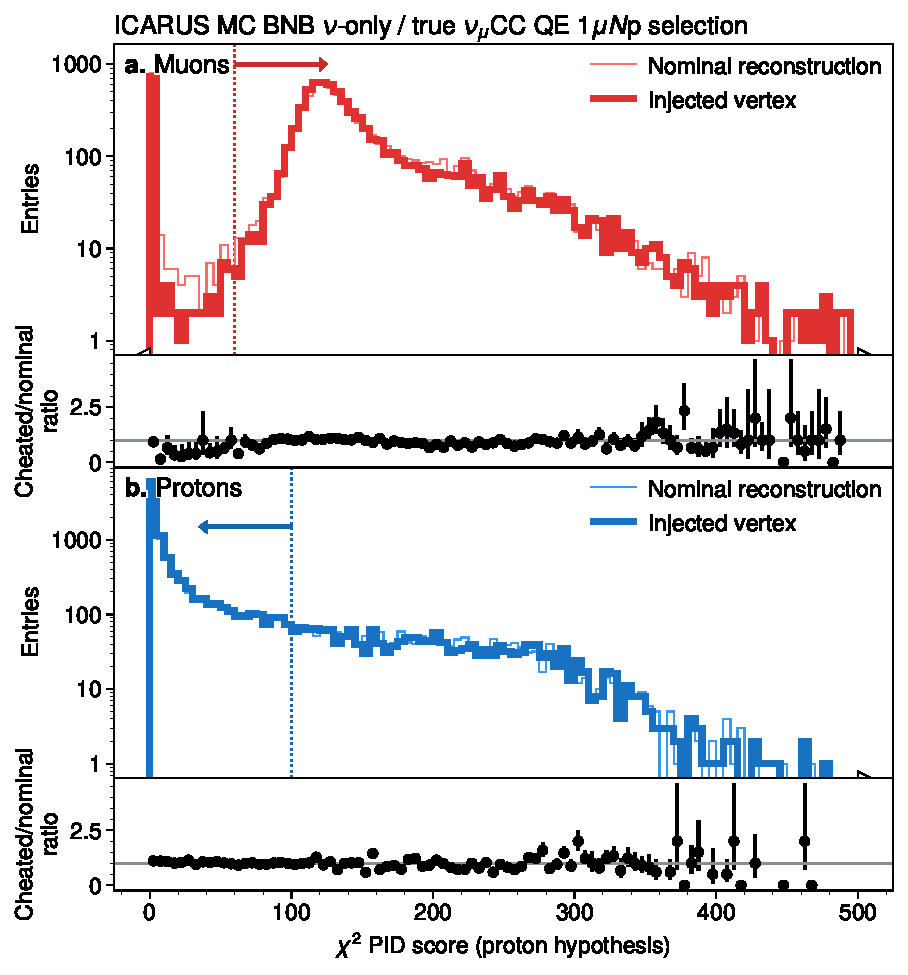
\includegraphics[width=0.5\linewidth]{pandora/chapter_4/chi2Proton_cheatedVertex.pdf}\label{fig:chi2Proton_cheatedVertex}}
    \subfloat[]{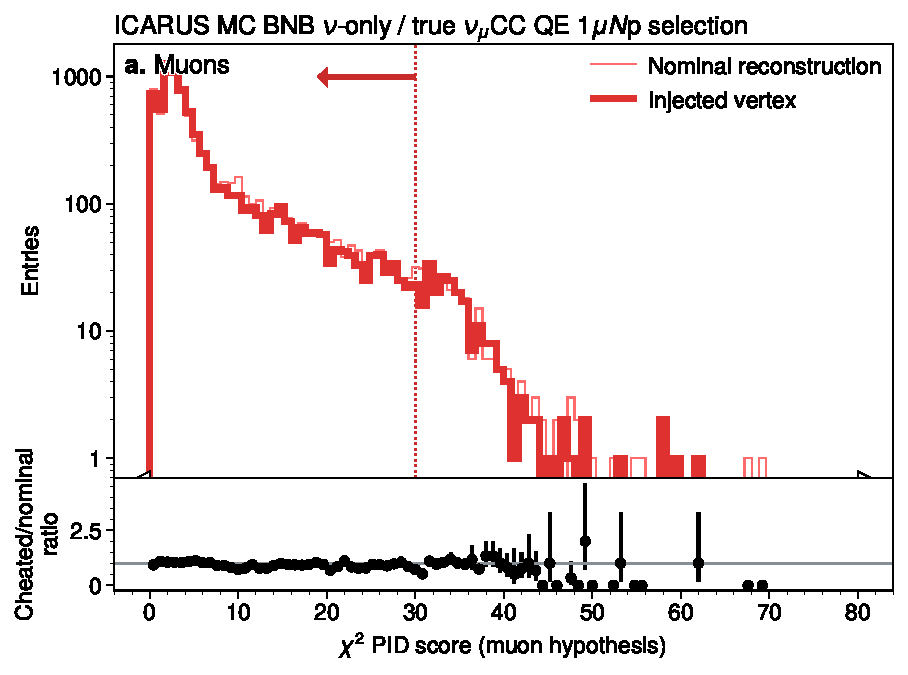
\includegraphics[width=0.5\linewidth, trim={0 -2.5cm 0 0}]{pandora/chapter_4/chi2Muon_cheatedVertex.pdf}\label{fig:chi2Muon_cheatedVertex}}
    \caption[Pid scores with the cheated vertex creation]{Particle identification score distributions for protons and muons. On the left the $\chi^2$ distribution, computed under the assumption of a proton track, is shown for both protons (blue) and muons (red), for the nominal (thin line) and cheated vertex reconstruction (thick line). The right plot shows the distribution of the $\chi^2$ score under the muon track hypothesis only for the muon population. The ratio is computed between the cheated reconstruction and the nominal one and shows no significant differences.  }
    \label{fig:chi2_cheatedVertex}
\end{sidewaysfigure}

% \begin{figure}
%     \centering
%     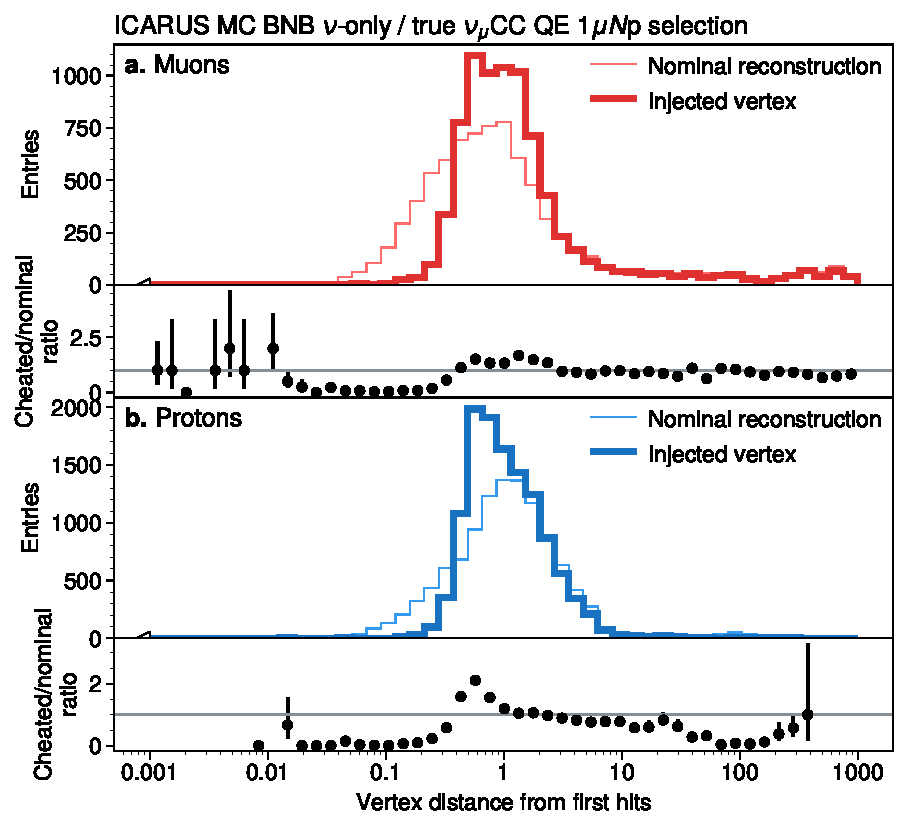
\includegraphics[width=0.85\linewidth]{pandora/chapter_4/vertexDistance_cheated.pdf}
%     \caption{}
%     \label{fig:vertexDistance}
% \end{figure}

% remark on \autoref{fig:vertexDistance}?

To strengthen this result, a parallel study was performed using a different sample of events with a completely different topology: electron neutrino charge-current quasi-elastic candidates, $\PGne$CC QE. The $\PGne$CC QE analysis reported an improvement in efficiency of ${\sim}\SI{7.3}{\percent}$, perfectly compatible with that found by this work \SI{7.0(8)}{\percent} \cite{Triozzi:2025_impactNueReconstruction, Sotgia:2025_cheatingPandoraStatus}. 

Finally, another confirmation of such a result can be found by comparing it with that presented in \autoref{sec:resultsLadder}. Although the methods described in the previous \autoref{sec:methods} and in this section aim to achieve two different results, these must be consistent with each other. In the previous section, the efficiency of each stage of reconstruction was computed, while in this section, it was assessed how much room for improvement there is for a single stage, namely the vertex reconstruction. 

It was in fact shown that the vertex creation step in the PandoraNeutrino reconstruction has an overall efficiency of ${\sim}\SI{91.9}{\percent}$. This is equivalent to affirming that the inefficiencies due to the incorrect vertex reconstruction account for approximately ${\sim}\SI{8.1}{\percent}$ of the total. This is coherent with the maximum efficiency gain that could be reached if the vertex reconstruction was perfect, which is computed in this section to be \SI{7.0(8)}{\percent}. 

\subsection{Future outlook: improving the vertex creation algorithm}

Having shown that the vertex reconstruction plays a central role in the event reconstruction chain and that there is a large overhead that can be gained from improving this individual step of the reconstruction, this section tries to draw a pathway to what the next steps should be in order to improve the vertex reconstruction, thereby improving the event reconstruction efficiency. This will surely prove core for the $\PGnGm$CC QE Np analysis channel, but also for many future analyses, such as an $\PGne$CC QE analysis, for which preliminary work is now being performed \cite{Triozzi:2025_impactNueReconstruction}. 

To improve the vertex reconstruction, there are two ways. One might take the currently existing algorithms, which are described in \autoref{sec:TPC_reco_gen}, and fine-tune their parameters and retrain the vertex selection algorithm: this is a valid solution, but this work highlights that the maximum improvement which can be achieved in such a way would result in a ${\sim}\SI{5}{\percent}$ boost in the event reconstruction efficiency. Another way is to adopt newer technologies, currently being developed within the Pandora software framework and tested in other LArTPC experiments, such as DUNE, to reinvent completely the way the vertex reconstruction is performed. Such tools employ the use of machine-learning-based technologies, such as Deep Neural Networks (DNNs) and Convolutional Neural Networks (CNNs). 

The idea of the deep learning vertex creation algorithm \cite{DUNE:2025wti} arises from two considerations. The first is that the filtered hits on the readout planes taken as input for the Pandora topological event reconstruction can be assimilated to 2D images, where each hit is a point on the image itself. The second is that, upon a visual inspection of the images of the neutrino interaction by a human expert, the interaction vertex is often, though not always, easily identified. Such a premise suggests that it is reasonable to assume that a machine-learning-based algorithm, employing deep convolutional neural networks, often used in the context of medical imaging \cite{ronneberger2015unetconvolutionalnetworksbiomedical,10.1007/978-3-319-24574-4_28}, would be well suited to automate this inherently visual task. 

The concept for this network design adopted here is to relate each hit to the interaction vertex: each hit contributes to the identification of the interaction vertex, and the network can learn reciprocal hit spatial correlations, providing context to the vertex identification. If the hit is defined as a pixel point of coordinates $(h_x, h_c)$, with $x$ being the drift coordinate and $c$ being the readout channel in $u$, $v$, and $w$, and the same is done for the true interaction vertex, $(v_x, v_c)$, it is possible to define a distance metric as \begin{equation}
    D = \frac{\sqrt{\qty(v_x - h_x)^2 + \qty(v_c - h_c)^2}}{\floor{\sqrt{2\qty(L - 1)}}}.
\end{equation} It should be noted that this definition of distance is scale-invariant, being divided by the characteristic dimension of the interaction $L$. This is core to allow the network to not learn any scale-related feature (i.e., not being correlated with the interaction scale). The computed distance is then allocated into one of 19 classes (see \autoref{fig:DLVertexAlgorithm}\ref{sub@fig:DLVertexAlgorithmClasses}). The network then tries to infer the class for each hit. Once the classes are inferred for each hit in the interaction, the class number provides each hit the information of its relative distance to the interaction vertex. This information is used to project rings of appropriate inner and outer radii, centred on each hit. The width of the rings depends on the distance of the hit from the reconstructed vertex and is useful to provide a weight for each hit: the furthest hits are supposedly less spatially correlated with the interaction features closer to the vertex; therefore, the accuracy in their distance to the vertex is supposed to be less. \autoref{fig:DLVertexAlgorithm}\ref{sub@fig:DLVertexAlgorithmHeatmap} shows the projected rings for three hits in the interaction. The reconstructed interaction vertex lies in the common region where the rings cross. 

\begin{figure}
    \centering
    \subfloat[]{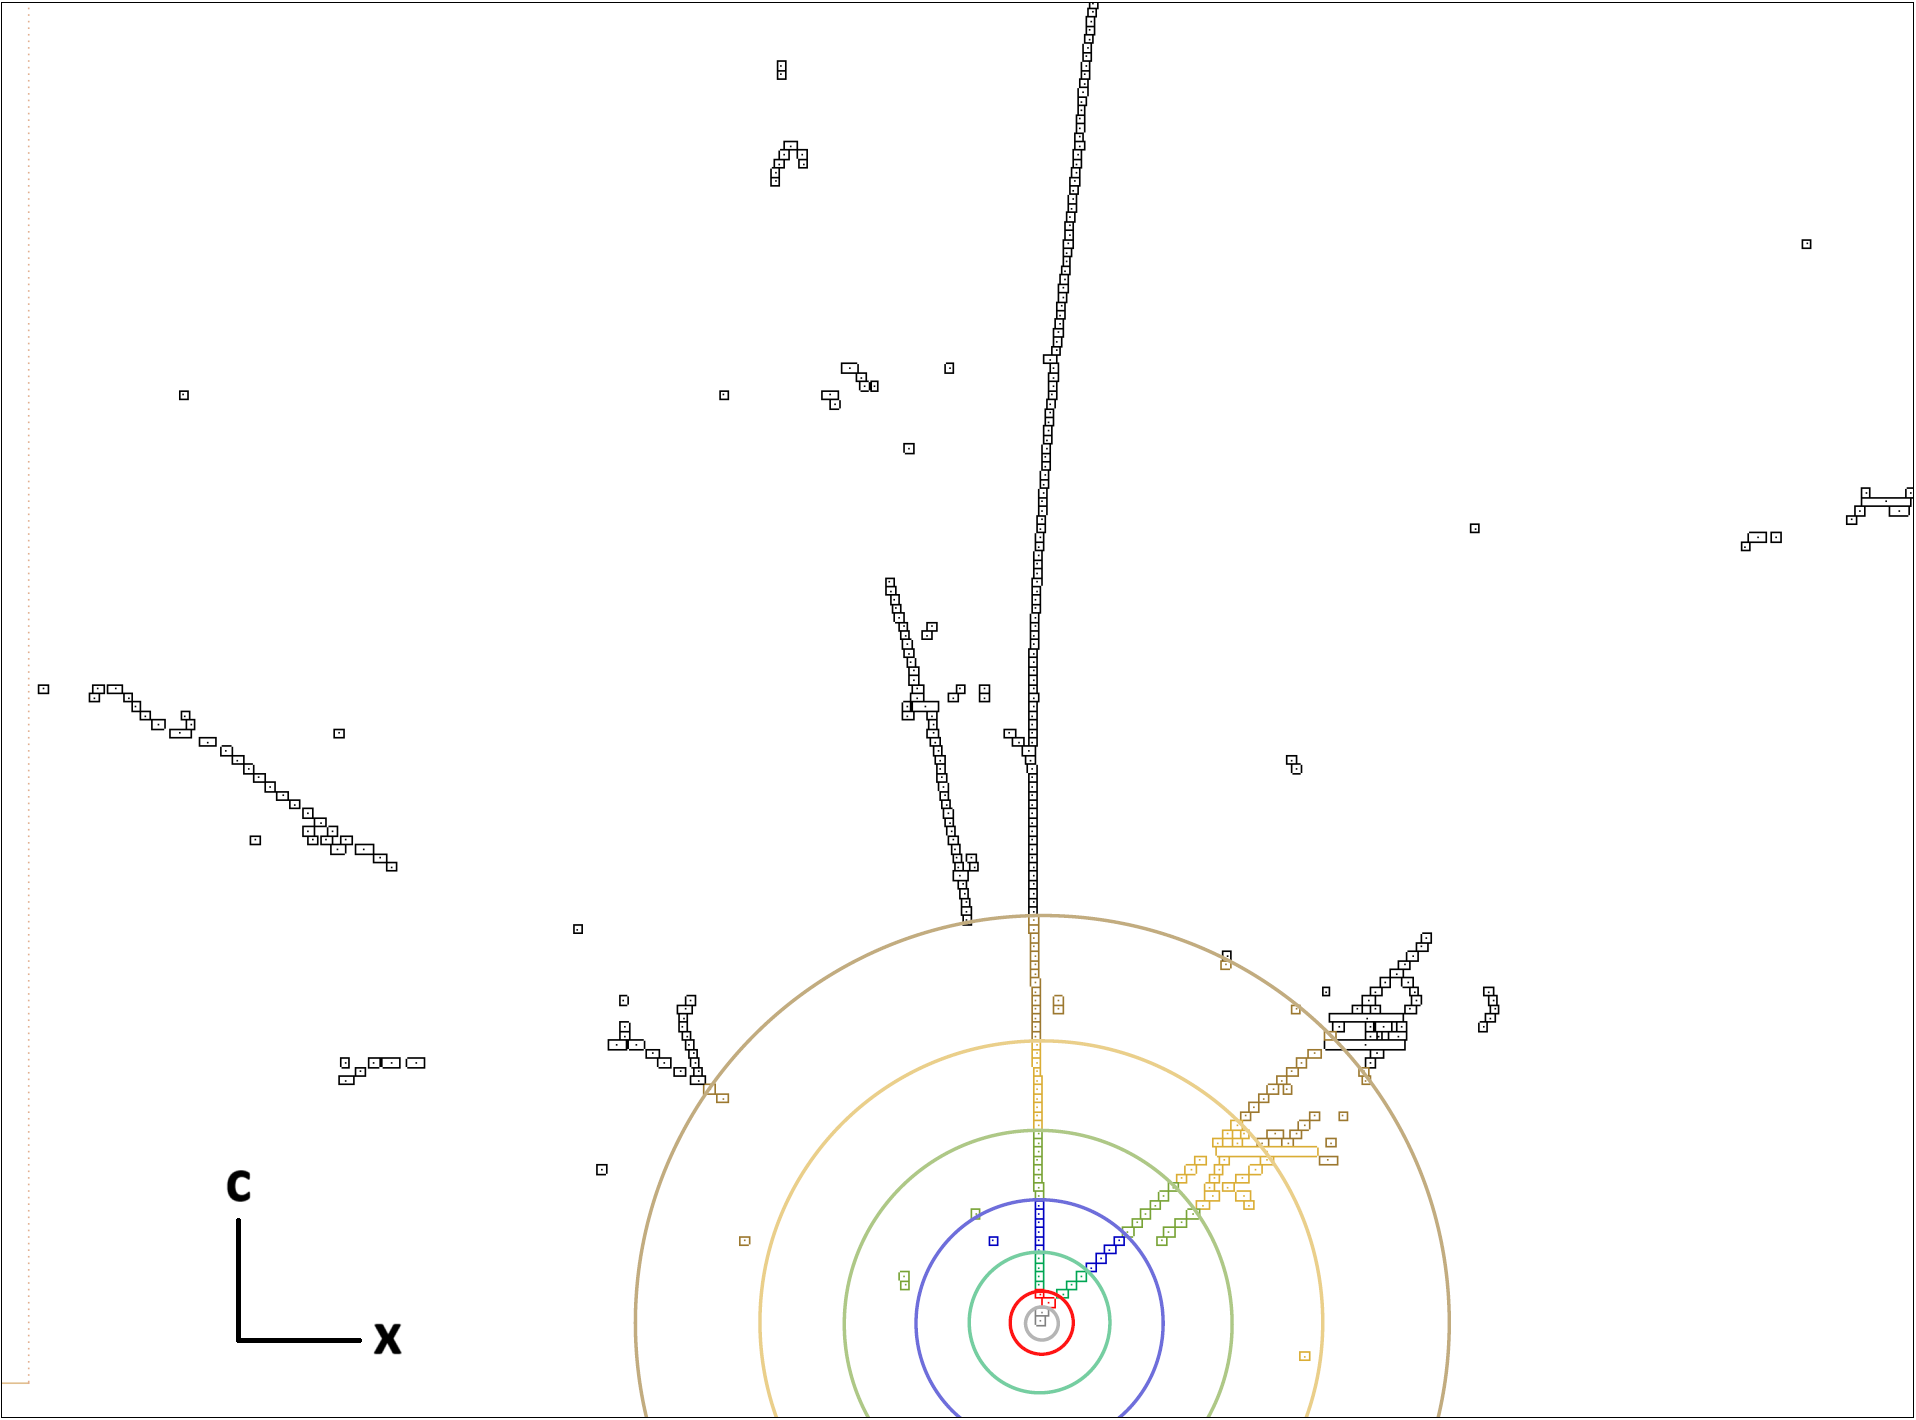
\includegraphics[width=0.5\linewidth]{pandora/vertex_DL/vtx_classes.png}\label{fig:DLVertexAlgorithmClasses}}
    \subfloat[]{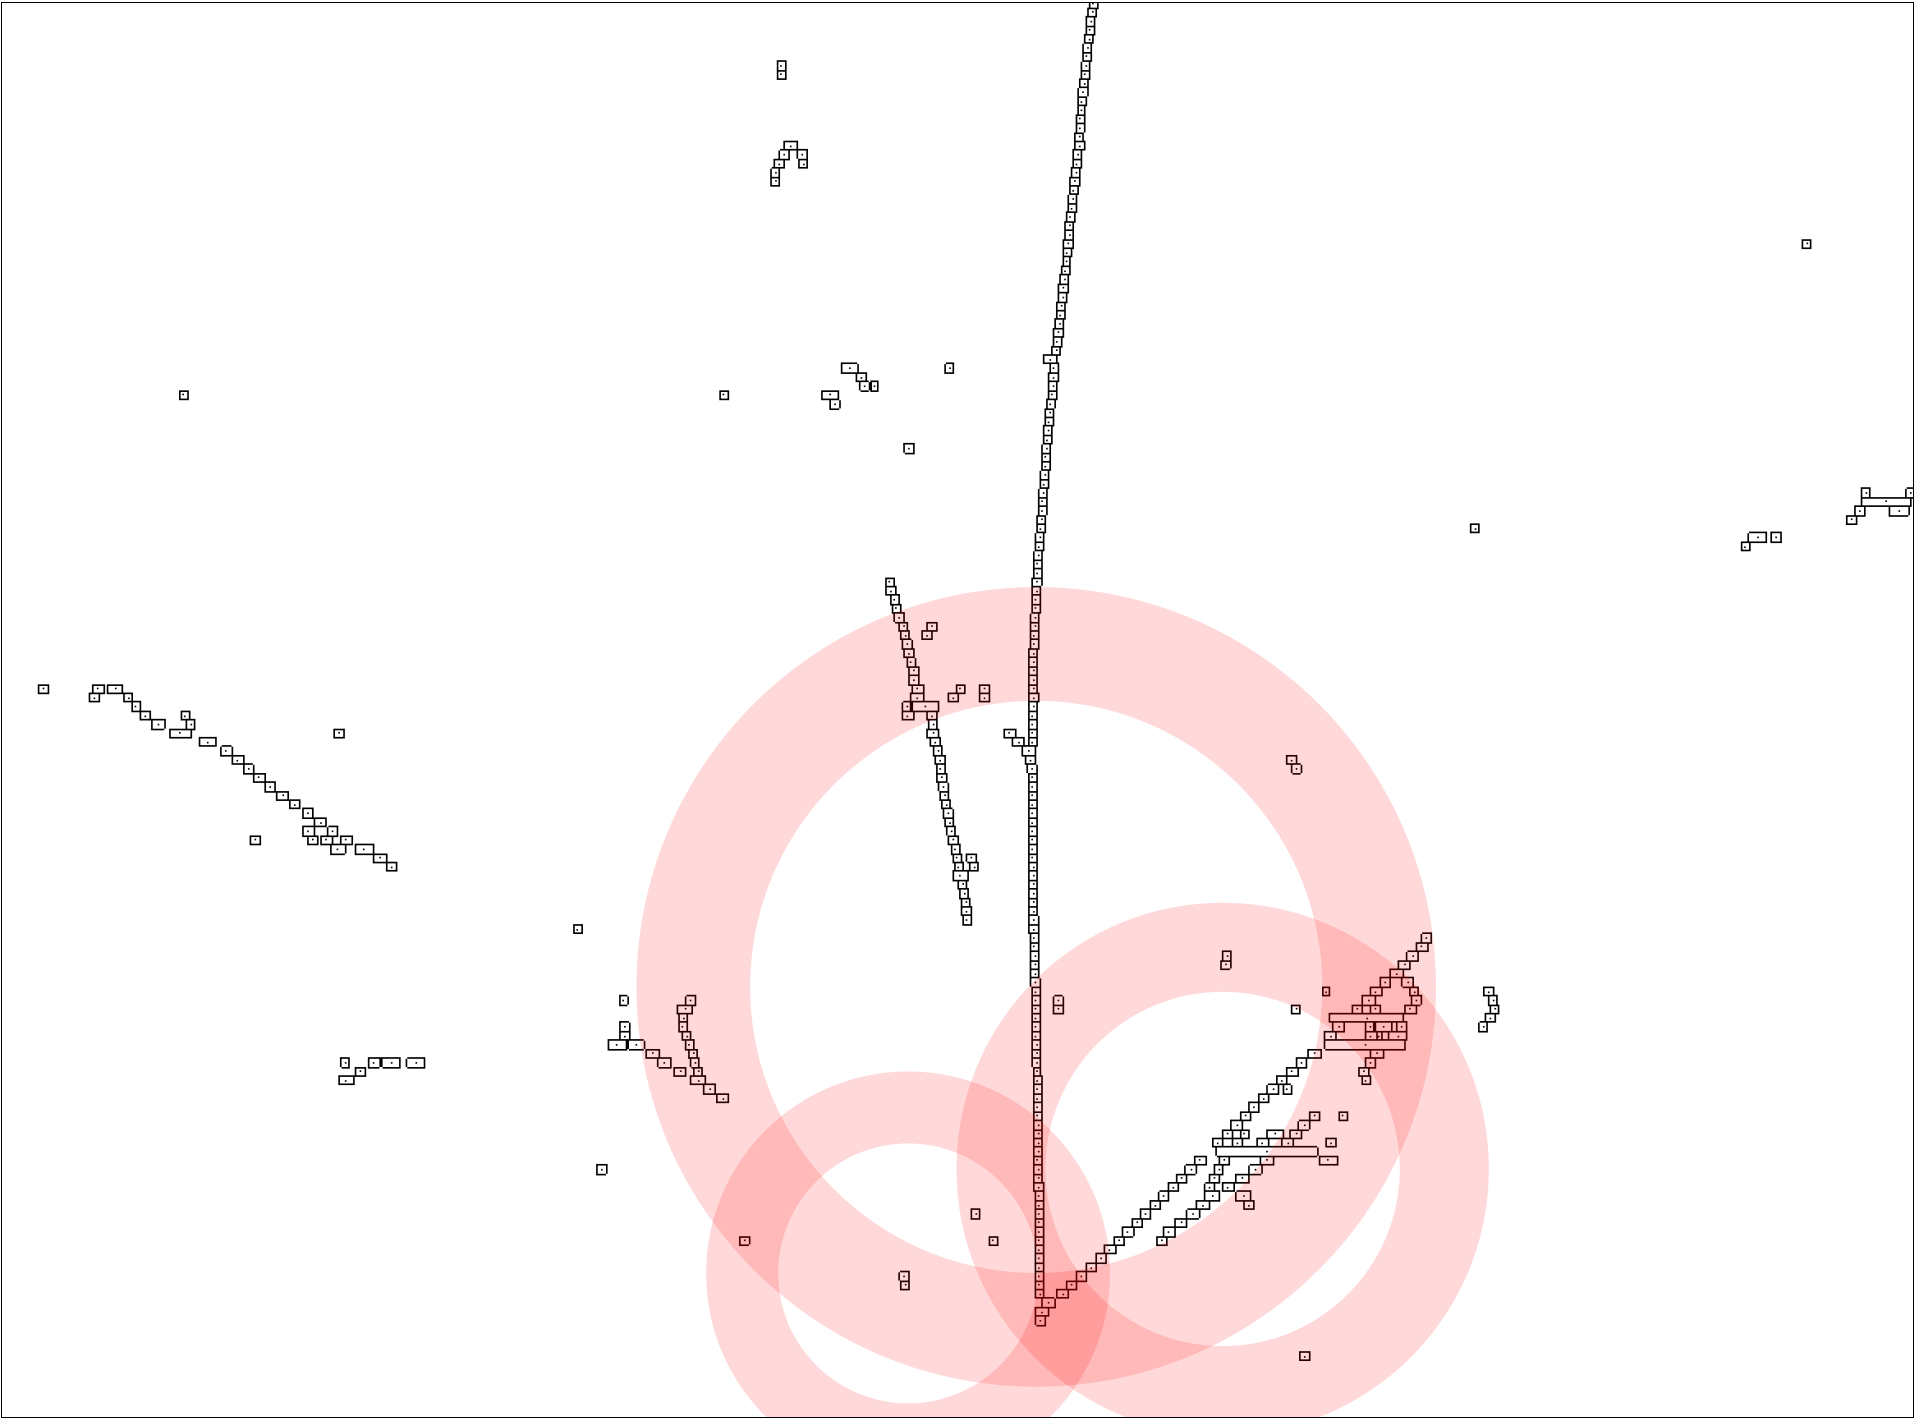
\includegraphics[width=0.5\linewidth]{pandora/vertex_DL/vtx_infer.png}\label{fig:DLVertexAlgorithmHeatmap}}
    \caption[Working principle of the DL vertex algorithm]{\ref{sub@fig:DLVertexAlgorithmClasses} shows the input hits and assignment of the first seven of the nineteen true distance classes for those hits. \ref{sub@fig:DLVertexAlgorithmHeatmap} shows a schematic of the heat map produced by three arbitrary hits during inference, for one view ($w$) of an event}
    \label{fig:DLVertexAlgorithm}
\end{figure}

Further details on the implementation and technicalities of the deep learning (DL) vertex algorithm are presented in Ref. \cite{DUNE:2025wti}. 

Implementing this algorithm, which in preliminary tests claims incredible performances, requires some attention. Firstly, it is important to remark that it was originally developed for use within DUNE, where the rate of cosmic-ray interaction is significantly lower. This means that a lower rate of cosmic contamination in neutrino interaction is present, helping the performance of the algorithm. This leads directly to the second remark. In order to both train the algorithm, and then use it in inference with real data, some upgrades are required on the reconstruction chain, to ensure that slices are created correctly and no particles get broken between interaction slices. 

% \section{Refining the slice creation tool}

Looking at the 


\begin{figure}
    \centering
    \subfloat[]{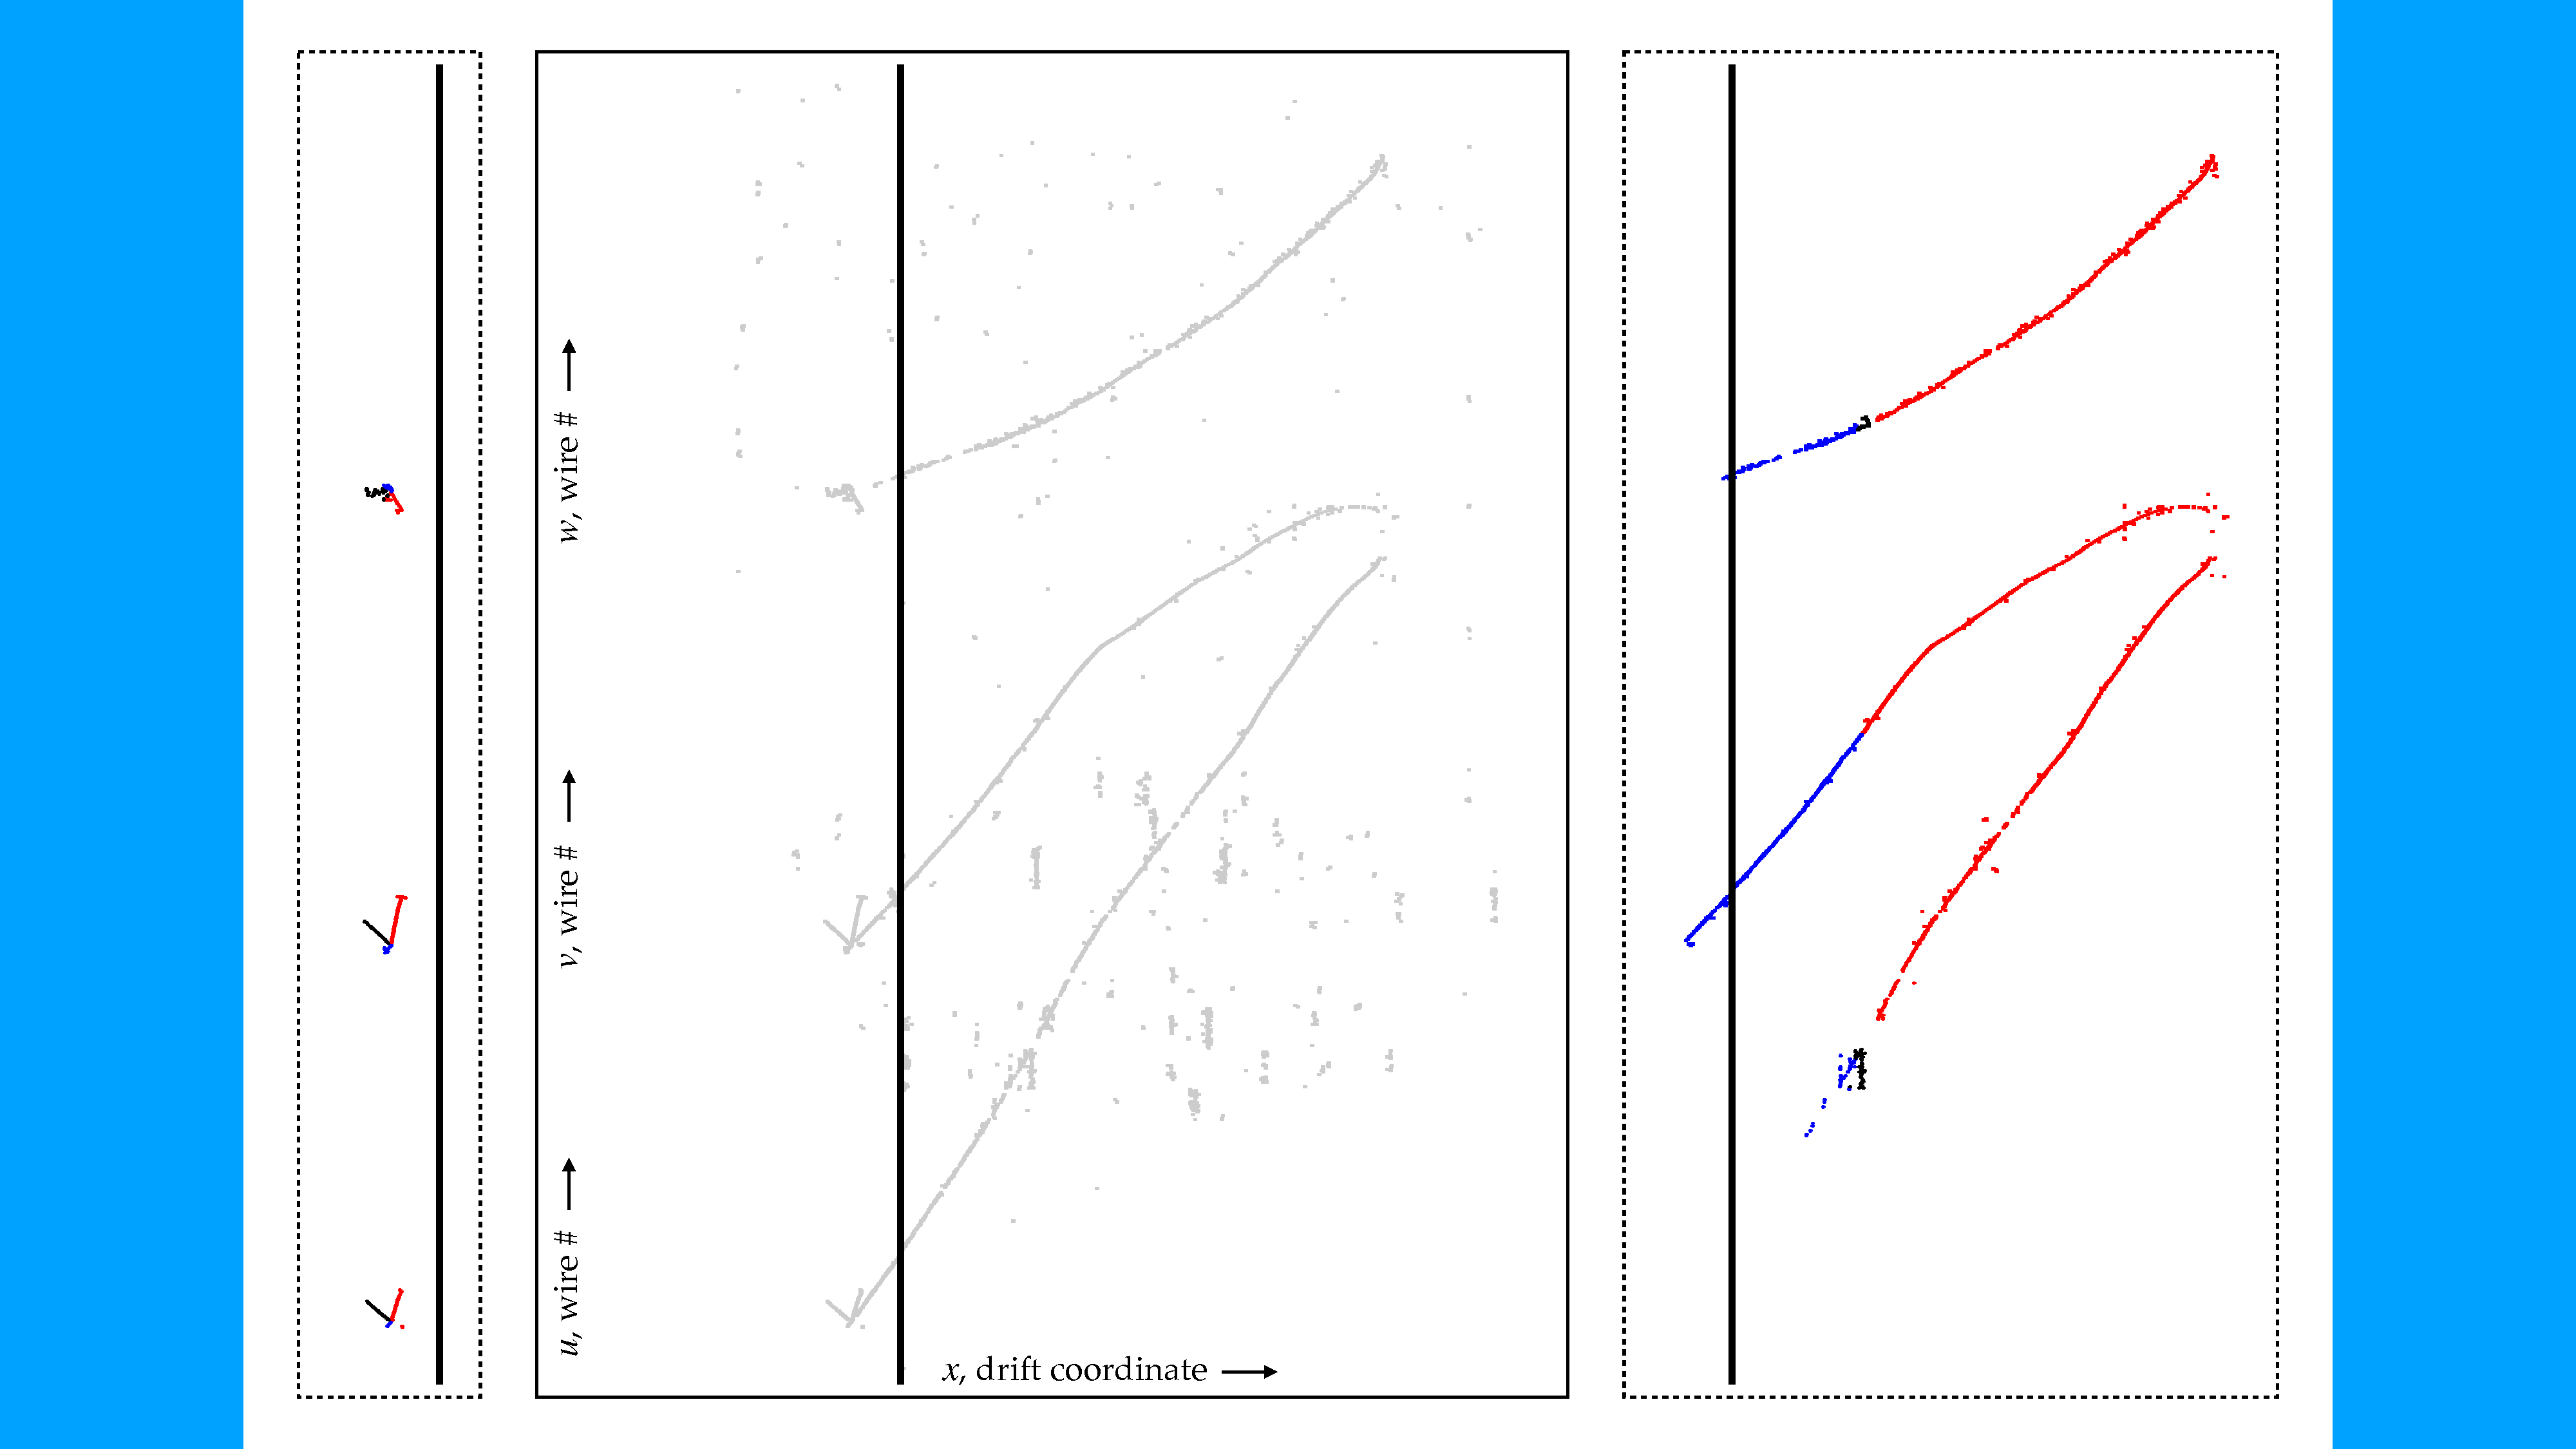
\includegraphics[width=0.9\linewidth,trim={7cm 1cm 7cm 1cm}, clip, page=1]{pandora/chapter_4/sliceIssue.pdf}}
    
    \subfloat[]{\includegraphics[width=0.9\linewidth,trim={7cm 3.5cm 7cm 3.5cm}, clip, page=2]{pandora/chapter_4/sliceIssue.pdf}}
    \caption[Examples of issues with the slice creation]{Two events where the slice cr4eation fails and two slices are created. Both events feature a ``noisy'' induction-1 ($w$) plane. }
    \label{fig:sliceIssue}
\end{figure}

